\documentclass[a4paper,12pt]{article}
\usepackage[a4paper,left=2cm,right=2cm]{geometry}
\usepackage[english]{babel}
\usepackage[latin1]{inputenc}
\usepackage{graphicx}
\usepackage[formats]{listings}
\setcounter{tocdepth}{2}
\lstdefinelanguage{Julia}{
      keywords = {function,type,end,if,else,return,elseif,@everywhere,@testset,@test,for,@parallel,@async,@sync,@elapsed}
}
\lstdefineformat{Julia}{%
\{ = \newline\indent,%
\} = \newline\noindent,%
?=\indent
}
\lstset{
language= Julia,
basicstyle=\footnotesize
}
\lstset{
language= Python,
basicstyle=\small
}
\begin{document}
\title{IN480 \hspace{0.5cm} Larstruct Module}
\author{Desiree Adiutori \and Alessia Giulia Cossu}
\maketitle
\tableofcontents
\newpage
\section*{Introduction}
\addcontentsline{toc}{section}{Introduction}
This module of LAR-CC library is about a hierarchical structures with LAR.
Hierarchical models of complex assemblies are generated by an aggregation of subassemblies, each one defined in a local coordinate system, and relocated by affine transformations of coordinates.

In this module there are:
\begin{itemize}
\item The \textbf{Affine transformations} are based on elementary matrices for affine transformation of vectors in any dimensional vector space, including translation, scaling and rotation;
\item The \textbf{Struct iterable class}, starting from an array representable geometric object, generates a new object representing the initial one in an alternative way, by means of specific fields attribution, e.g. body, box, etc..
\item The \textbf{structure to LAR conversion} is based on functions for embedding two-dimensional LAR model in 3D space and remove duplicate faces, vertices and cells of geometric object. 
\end{itemize}
In the next sections the main functions of the module will be shown through the API. Furthermore, each function will be proposed to convert code from the Python language to Julia, parallelization, some unit tests and the study of execution times.
\newpage
\section{API}
\begin{itemize}
\item \textbf{larApply}(Matrix)(Tuple)$\rightarrow$ Tuple,

through the affine matrix given in input, it performs an affine transformation and returns in output a tuple containing two arrays: the list of the transformed coordinates of the vertices and a cell vector.
\item \textbf{evalStruct}(Struct)$\rightarrow$ Array,

analyzes the elements contained in the Struct object and returns an array containing the main data structures. Each structure is described by an array containing two arrays: the list of the transformed coordinates of the vertices and a cell vector.
\item  \textbf{vcode}(Int)(Array)$\rightarrow$String,

generates the function that approximates each element of the data structure to which it is applied. the approximation occurs with precision given by the entire input data. It transforms the data structure obtained in string to be returned to output.
\item \textbf{struct2lar}(Struct)$\rightarrow$ Array,

it extracts the elements composing the input and combines them into a single element represented by the output array, where: the first element contains the array of the coordinates of the vertices of all the objects present, the second contains vectors of larger cells without duplicates of vertices. If we are in 3D: the third element contains the 3D cells, this array can add elements depending on how many were added to the first one.
\item \textbf{larRemoveVertices}(Array, Array)$\rightarrow$ (Array,Array)

takes in input arrays of vertices and cells and returns them private of their duplicates
\item \textbf{larEmbed}(Int)(Tuple)$\rightarrow$ Tuple,
if the input n is such that n>0 the function generated increases n the size of the object to which it is applied, otherwise it reduces the size of n.
\item \textbf{larBoundary}(Struct)$\rightarrow$ (Array,Array,Array)

apply struct2lar to the input, if the output has dimension 3, the function returns a tuple containing the 3 outputs, otherwise it returns a string containing an error message.
\item \textbf{embedStruct}(Int)(Struct)$\rightarrow$ Struct,

creates a copy of the object to which it is applied, increases its size, as much as the value entered in input and returns the new object created.
\end{itemize}
\textbf{Internal Functions} 
\begin{itemize}
\item \textbf{checkStruct}(Array)$\rightarrow$ Int 
\item \textbf{traversal}(Matrix,Array,Struct,Array)$\rightarrow$ Array
\item \textbf{prepKey}(String)$\rightarrow$String 
\item \textbf{fixedPrec}(Int)$\rightarrow$ String
\item \textbf{removeDups}(Array)$\rightarrow$ Array
\end{itemize}
\begin{figure}[h!]
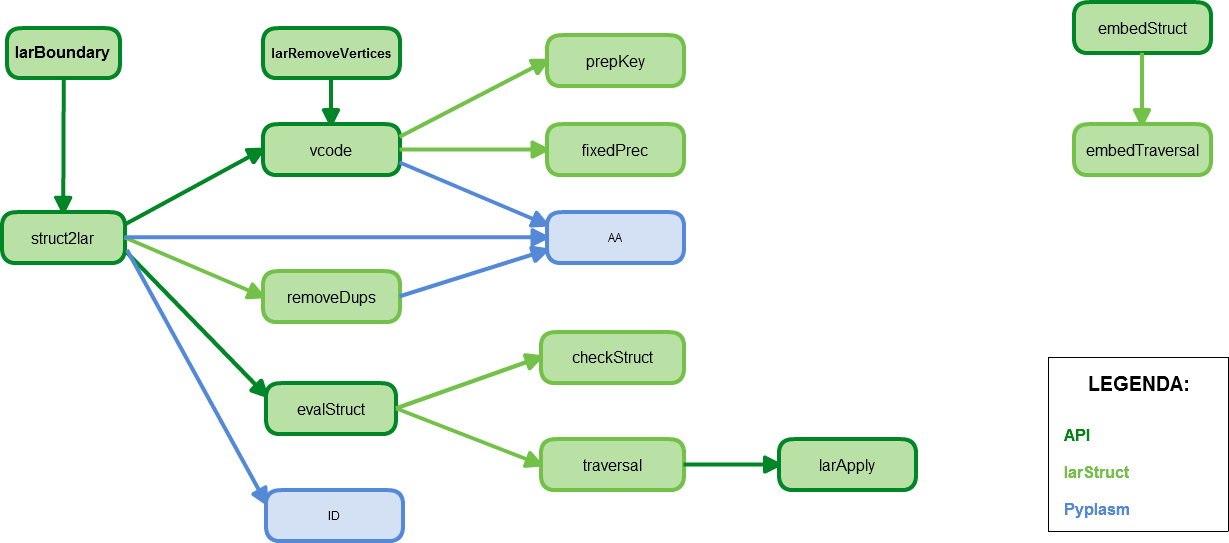
\includegraphics[width=17cm, scale=0.5]{larStruct.png}
\end{figure}
\newpage
\section{Implementation}
This section shows the translation from the Python language to Julia, of some of the most important module functions. The Results section is divided into two parts: the first shows the performance graphs of the functions, run on the 'Tesla' computer with 30 processors, where the input is increased by increasing the body of the objects of Struct type, through the function:
 \begin{lstlisting}[language=Julia,format=Julia]
 function addn2D(n,model){
	 body=[ ]
	 for i in range(1,n){
	     el=[ ]
	     matrix=rand(1:3)
	     if matrix==1{
	     	 x=rand(1:10)/10
	     	 y=rand(1:10)/10
	     	append!(el,larApply(t(x,y))(model))
		append!(body,[el])}
	     elseif matrix ==2{
	     	     x=rand(1:10)/10
	    	     y=rand(1:10)/10
	     	    append!(el,larApply(s(x,y))(model))
		    append!(body,[el])}
	     elseif matrix ==3{
	     	     x=rand(1:10)
		     append!(el,larApply(r(pi/x))(model))
		    append!(body,[el])}
	     end}
	 end
	 a=Struct(body)
	return a}
end
 \end{lstlisting}
In the second part the graphs refer to functions run on a personal computer with 4 processors, where the increase in input was made starting from a function external to the '' larCuboids '' module by:
 \begin{lstlisting}[language=Julia,format=Julia]
using Pycall
@pyimport larlib as lar
 input=[ ]
 for i in range(0,3){
 	append!(input,lar.larCuboids([10^i,10^i]))
	append!(input,lar.larCuboids([2*10^i,2*10^i]))
	append!(input,lar.larCuboids([5*10^i,5*10^i]))}
end
 \end{lstlisting}
The function to calculate the execution time is:
  \begin{lstlisting}[language=Julia,format=Julia]
  function Time(f::Function,args){
  @elapsed f(args...)
  t=[]
  for i in range(1,10){
  push!(t,@elapsed f(args...))}
  end
  m=mean(t)
  return m}
  end
   \end{lstlisting}
The requirements for running scripts are:
\begin{itemize}
\item using Base.Test
\item using Plots
\item using Distributions
\end{itemize}
from the Julia terminal on Tesla:
\begin{verbatim}
 addprocs(29)
 \end{verbatim}
or from the shell run Julia with the command:
  \begin{verbatim}
   julia -p 30
   \end{verbatim}
from the Julia terminal on personal computer: 
\begin{verbatim}
 addprocs(3) 
 \end{verbatim}
  or from the shell run Julia with the command:
  \begin{verbatim}
   julia -p 4
    \end{verbatim}
\subsection{checkStruct}
\subsubsection{Conversion}
\textbf{\emph{Python}}
 \lstset{language=Python}
\begin{lstlisting}
def checkStruct(lst):
   obj = lst[0]
   if(isinstance(obj,tuple) or isinstance(obj,list)):
      dim = len(obj[0][0])
   elif isinstance(obj,Model): 30
      dim = obj.n    
   elif isinstance(obj,Mat): 
      dim = obj.shape[0]-1    
   elif isinstance(obj,Struct): 
      dim = len(obj.box[0])    
   return dim
\end{lstlisting}
\textbf {\emph{Julia}}
\begin{lstlisting}[language=Julia, format=Julia]
function checkStruct(lst) {
obj = lst[1]
if isa(obj,Matrix) {
dim=size(obj)[1]-1 }
   elseif(isa(obj,Tuple) || isa(obj,Array)) {
      dim=length(obj[1][1]) }
   elseif isa(obj,Struct){
      dim=length(obj.box[1])}
   end 
   return dim }
end
\end{lstlisting}
\subsubsection{Parallelization}
\begin{lstlisting}[language=Julia, format=Julia]
function pcheckStruct(lst) {
obj = lst[1]
if isa(obj,Matrix) {
dim=size(obj)[1]-1 }
   elseif(isa(obj,Tuple) || isa(obj,Array)) {
      dim=length(obj[1][1]) }
   elseif isa(obj,pStruct){
      dim=length(obj.box[1])}
   end 
   return dim }
end
\end{lstlisting}
\subsubsection{Unit-Test}
\begin{lstlisting}[language=Julia, format=Julia]
@testset "checkStruct" begin{
 list=([[0.575,-0.175],[0.575,0.175],[0.925,-0.175],[0.925,0.175]],{
 [[0,1,2,3]])}
@test checkStruct(list)==length(list[1][1][1])
@test typeof(checkStruct(list))==Int
end
\end{lstlisting}
\newpage
\subsection{larApply}
\subsubsection{Conversion}
\textbf{Python}
\begin{lstlisting}[language=Python,format=Julia]
def t(*args): {
    d = len(args)
    mat = scipy.identity(d+1)
    for k in range(d): {
        mat[k,d] = args[k]}
    return mat.view(Mat)}

def s(*args): {
    d = len(args)
    mat = scipy.identity(d+1)
    for k in range(d): {
        mat[k,k] = args[k]}
    return mat.view(Mat)}

def r(*args): {
    args = list(args)
    n = len(args)
    if n == 1: # rotation in 2D{
        angle = args[0]; cos = COS(angle); sin = SIN(angle)
        mat = scipy.identity(3)
        mat[0,0] = cos;    mat[0,1] = -sin;
        mat[1,0] = sin;    mat[1,1] = cos;}
     if n == 3: # rotation in 3D{
        mat = scipy.identity(4)
        angle = VECTNORM(args); axis = UNITVECT(args)
        cos = COS(angle); sin = SIN(angle)
        if axis[1]==axis[2]==0.0:    # rotation about x{
            mat[1,1] = cos;    mat[1,2] = -sin;
            mat[2,1] = sin;    mat[2,2] = cos;}
        elif axis[0]==axis[2]==0.0:    # rotation about y{
            mat[0,0] = cos;    mat[0,2] = sin;
            mat[2,0] = -sin;    mat[2,2] = cos;}
        elif axis[0]==axis[1]==0.0:    # rotation about z{
            mat[0,0] = cos;    mat[0,1] = -sin;
            mat[1,0] = sin;    mat[1,1] = cos;}
        else:        # general 3D rotation (Rodrigues' rotation formula)    {
            I = scipy.identity(3) ; u = axis
            Ux = scipy.array([
                [0,        -u[2],      u[1]],
                [u[2],        0,     -u[0]],
                [-u[1],     u[0],         0]])
            UU = scipy.array([
                [u[0]*u[0],    u[0]*u[1],    u[0]*u[2]],
                [u[1]*u[0],    u[1]*u[1],    u[1]*u[2]],
                [u[2]*u[0],    u[2]*u[1],    u[2]*u[2]]])
            mat[:3,:3] = cos*I + sin*Ux + (1.0-cos)*UU}
     return mat.view(Mat)}

def larApply(affineMatrix):{
def larApply0(model):{
        if isinstance(model,Model):{
            V = scipy.dot(array([v+[1.0] for v in model.verts]), 
            affineMatrix.T).tolist()
            V = [v[:-1] for v in V]
            CV = copy.copy(model.cells)
            return Model((V,CV))}
        elif isinstance(model,tuple) or isinstance(model,list):{
            if len(model)==2: V,CV = model
            elif len(model)==3: V,CV,FV = model
            V=scipy.dot([list(v)+[1.0]for v in V],affineMatrix.T).tolist()
            if len(model)==2: return [v[:-1] for v in V],CV
            elif len(model)==3: return [v[:-1] for v in V],CV,FV}
    return larApply0
\end{lstlisting}
\textbf{Julia}
\begin{lstlisting}[language=Julia,format=Julia]
function t(args...){
	d=length(args)
	mat=eye(d+1)
	for k in range(1,d){
        	mat[k,d+1]=args[k]}
	end
	return mat}
end

function s(args...){
	d=length(args)
	mat=eye(d+1)
	for k in range(1,d){
		mat[k,k]=args[k]}
	end
	return mat}
end

function r(args...){
    args = collect(args)
    n = length(args)
    if n == 1 # rotation in 2D{
        angle = args[1]; COS = cos(angle); SIN = sin(angle)
        mat = eye(3)
        mat[1,1] = COS;    mat[1,2] = -SIN;
        mat[2,1] = SIN;    mat[2,2] = COS;}
    end
     if n == 3 # rotation in 3D{
        mat = eye(4)
        angle = norm(args); axis = normalize(args)
        COS = cos(angle); SIN= sin(angle)
        if axis[2]==axis[3]==0.0    # rotation about x{
            mat[2,2] = COS;    mat[2,3] = -SIN;
            mat[3,2] = SIN;    mat[3,3] = COS;}
        elseif axis[1]==axis[3]==0.0   # rotation about y{
            mat[1,1] = COS;    mat[1,3] = SIN;
            mat[3,1] = -SIN;    mat[3,3] = COS;}
        elseif axis[1]==axis[2]==0.0    # rotation about z{
            mat[1,1] = SIN;    mat[1,2] = -SIN;
            mat[2,1] = COS;    mat[2,2] = COS;}
           else{
	    I=eye(3); u=axis
	    Ux=[0 -u[3] u[2] ; u[3] 0 -u[1] ;  -u[2] u[1] 1]
	    UU =[u[1]*u[1]    u[1]*u[2]   u[1]*u[3];
             u[2]*u[1]    u[2]*u[2]   u[2]*u[3];
             u[3]*u[1]    u[3]*u[2]   u[3]*u[3]]
	    mat[1:3,1:3]=COS*I+SIN*Ux+(1.0-COS)*UU}
		end}
	end
return mat}
end
\end{lstlisting}
\begin{lstlisting}[language=Julia]
function larApply(affineMatrix)
   function larApply0(model)
      if length(model)==2
         V,CV=model
      elseif length(model)==3
         V,CV,FV = model
      end
      V1=Array{Float64}[]
      for (k,v) in enumerate(V)
         append!(v,[1.0])
         push!(V1,vec((v')*transpose(affineMatrix)))
         pop!(V[k])
         pop!(V1[k])
	   end
      if length(model)==2
         return V1,CV
      elseif length(model)==3
         return V1,CV,FV
      end
   end 
   return larApply0
end
\end{lstlisting}
\subsubsection{Parallelization}
The functions for the affine transformation matrices are the same as in the sequential case.
\begin{lstlisting}[language=Julia]
@everywhere function plarApply(affineMatrix)
	function plarApply0(model)
	    if length(model)==2
	       V,CV=deepcopy(model)
	    elseif length(model)==3
      	    	   V,CV,FV = deepcopy(model)
	    end
	   V1=Array{Float64}[ ]
	   V1=@sync @parallel (append!)for v in V
	    	       append!(v,[1.0])
	    	      [collect(vec((v')*transpose(affineMatrix)))]
		end
		for v in V1
			pop!(v)
		end	    
	     if length(model)==2
		return fetch(V1),CV
	     elseif length(model)==3
		return V1,CV,FV
	      end
	 end 
	 return plarApply0
end
\end{lstlisting}
\subsubsection{Unit-Test}
\begin{lstlisting}[language=Julia]
square=([[0,0],[0,1],[1,0],[1,1]],[[0,1,2,3]])
cubes=([[0,0,0],[0,0,1],[0,1,0],[0,1,1],[1,0,0],[1,0,1],[1,1,0],[1,1,1]],
       [[0,1,2,3,4,5,6,7]])

@testset "larApply Tests" begin
   @testset "2D" begin
      @testset "larApply Translation 2D" begin
      @test typeof(larApply(t(-0.5,-0.5))(square))==Tuple{Array{Array{
                 Float64,N} where N,1},Array{Array{Int64,1},1}}
      @test larApply(t(-0.5,-0.5))(square)==([[-0.5,-0.5],[-0.5,0.5],
           [0.5,-0.5],[0.5,0.5]],[[0,1,2,3]])
   end
      @testset "larApply Scaling 2D" begin
         @test typeof(larApply(s(-0.5,-0.5))(square))==Tuple{Array{Array{
                  Float64,N} where N,1},Array{Array{Int64,1},1}}
         @test larApply(s(-0.5,-0.5))(square)==([[0.0,0.0],[0.0,-0.5],
                [-0.5,0.0],[-0.5,-0.5]],[[0,1,2,3]])
      end
      @testset "larApply Rotation 2D" begin
         @test typeof(larApply(r(0))(square))==Tuple{Array{Array{
                 Float64,N}  where N,1},Array{Array{Int64,1},1}}
         @test larApply(r(0))(square)==square
      end
   end

   @testset "3D" begin
      @testset "larApply Translation 3D" begin
         @test typeof(larApply(t(-0.5,-0.5,-0.5))(cubes))==Tuple{Array{
               Array{Float64,N} where N,1},Array{Array{Int64,1},1}}
         @test larApply(t(-0.5,-0.5,-0.5))(cubes)==([[-0.5,-0.5,-0.5],
               [-0.5,-0.5,0.5],[-0.5,0.5,-0.5],[-0.5,0.5,0.5],
               [0.5,-0.5,-0.5],[0.5,-0.5,0.5],[0.5,0.5,-0.5],
               [0.5,0.5,0.5]],[[0,1,2,3,4,5,6,7]])
      end 
	
      @testset "larApply Scaling 3D" begin
         @test typeof(larApply(s(-0.5,-0.5,-0.5))(cubes))==Tuple{Array{
               Array{Float64,N} where N,1},Array{Array{Int64,1},1}}
         @test larApply(s(-0.5,-0.5,-0.5))(cubes)==([[0.0,0.0,0.0],
                 [0.0,0.0,-0.5],[0.0,-0.5,0.0],[0.0,-0.5,-0.5],
                 [-0.5,0.0,0.0],[-0.5,0.0,-0.5],[-0.5,-0.5,0.0],
                 [-0.5,-0.5,-0.5]],[[0,1,2,3,4,5,6,7]])
      end
	
      @testset "larApply Rotation 3D" begin
         @test typeof(larApply(r(pi,0,0))(cubes))==Tuple{Array{Array{
                Float64,N} where N,1},Array{Array{Int64,1},1}}
\end{lstlisting}
\hspace{2cm} \textbf{@test}    larApply(r(pi,0,0))(cubes)[1]\ $\approx$ [[0.0,0.0,0.0],[0.0,-1.22465e-16,-1.0],
\begin{lstlisting}[language=Julia]
              [0.0,-1.0,1.22465e-16],[0.0,-1.0,-1.0],[1.0,0.0,0.0],
              [1.0,-1.22465e-16,-1.0],[1.0,-1.0,1.22465e-16],
              [1.0,-1.0,-1.0]]
          end
       end

square=([[0,0],[0,1],[1,0],[1,1]],[[0,1,2,3]])
cubes=([[0,0,0],[0,0,1],[0,1,0],[0,1,1],[1,0,0],[1,0,1],[1,1,0],
         [1,1,1]],[[0,1,2,3,4,5,6,7]])
@testset "plarApply Tests" begin
   @testset "2D" begin	
      @testset "plarApply Translation 2D" begin
         @test typeof(plarApply(t(-0.5,-0.5))(square))==Tuple{Array{
                    Array{Float64,1},1},Array{Array{Int64,1},1}}
         @test plarApply(t(-0.5,-0.5))(square)==([[-0.5,-0.5],[-0.5,0.5],
                    [0.5,-0.5],[0.5,0.5]],[[0,1,2,3]])
      end 
	
      @testset "plarApply Scaling 2D" begin
         @test typeof(plarApply(s(-0.5,-0.5))(square))==Tuple{Array{
                   Array{Float64,1},1},Array{Array{Int64,1},1}}
         @test plarApply(s(-0.5,-0.5))(square)==([[0.0,0.0],[0.0,-0.5],
                   [-0.5,0.0],[-0.5,0.5]],[[0,1,2,3]])
      end
	
      @testset "plarApply Rotation 2D" begin
         @test typeof(plarApply(r(0))(square))==Tuple{Array{Array{
                   Float64,1},1},Array{Array{Int64,1},1}}
         @test plarApply(r(0))(square)==square
      end
   end
  @testset "3D" begin
    @testset "plarApply Translation 3D" begin
      @test typeof(plarApply(t(-0.5,-0.5,-0.5))(cubes))==Tuple{Array{
                 Array{Float64,1},1},Array{Array{Int64,1},1}}
      @test plarApply(t(-0.5,-0.5,-0.5))(cubes)==([[-0.5,-0.5,-0.5],
                 [-0.5,-0.5,0.5],[-0.5,0.5,-0.5],[-0.5,0.5,0.5],
                 [0.5,-0.5,-0.5],[0.5,-0.5,0.5],[0.5,0.5,-0.5],
                 [0.5,0.5,0.5]],[[0,1,2,3,4,5,6,7]])
    end 
    @testset "plarApply Scaling 3D" begin
      @test typeof(plarApply(s(-0.5,-0.5,-0.5))(cubes))==Tuple{Array{
                 Array{Float64,1},1},Array{Array{Int64,1},1}}
      @test plarApply(s(-0.5,-0.5,-0.5))(cubes)==([[0.0,0.0,0.0],
                 [0.0,0.0,-0.5],[0.0,-0.5,0.0],[0.0,-0.5,-0.5],
                 [-0.5,0.0,0.0],[-0.5,0.0,-0.5],[-0.5,-0.5,0.0],
                 [-0.5,-0.5,-0.5]],[[0,1,2,3,4,5,6,7]])
    end
    @testset "plarApply Rotation 3D" begin
      @test typeof(plarApply(r(pi,0.0,0.0))(cubes))==Tuple{Array{Array{
                    Float64,1},1},Array{Array{Int64,1},1}}
 \end{lstlisting}
\hspace{1.35cm} \textbf{@test} plarApply(r(pi,0,0))(cubes)[1]$\approx$[[0.0,0.0,0.0],[0.0,-1.22465e-16,1.0],
\begin{lstlisting}[language=Julia]
           [0.0,-1.0,1.22465e-16],[0.0,-1.0,-1.0],[1.0,0.0,0.0],
           [1.0,-1.22465e-16,-1.0],[1.0,-1.0,1.22465e-16],
           [1.0,-1.0,-1.0]]
       end
     end
end
\end{lstlisting}
\subsubsection{Results}
\textbf{PC}
\begin{lstlisting}[language=Julia,format=Julia]
times=[ ]
ptimes=[ ]
for i in range(1,length(l)){
    append!(times,Time(larApply(t(-0.5,-0.5)),l[i]))}
end
for i in range(1,length(l)){
    append!(ptimes,Time(plarApply(t(-0.5,-0.5)),l[i]))}
end

plot(times,xlabel="input",xlims=(0,length(times)+2),{?ylabel="time(s)",label=["Serial"])
\end{lstlisting}
\newpage
\begin{figure}[ht!]
\centering
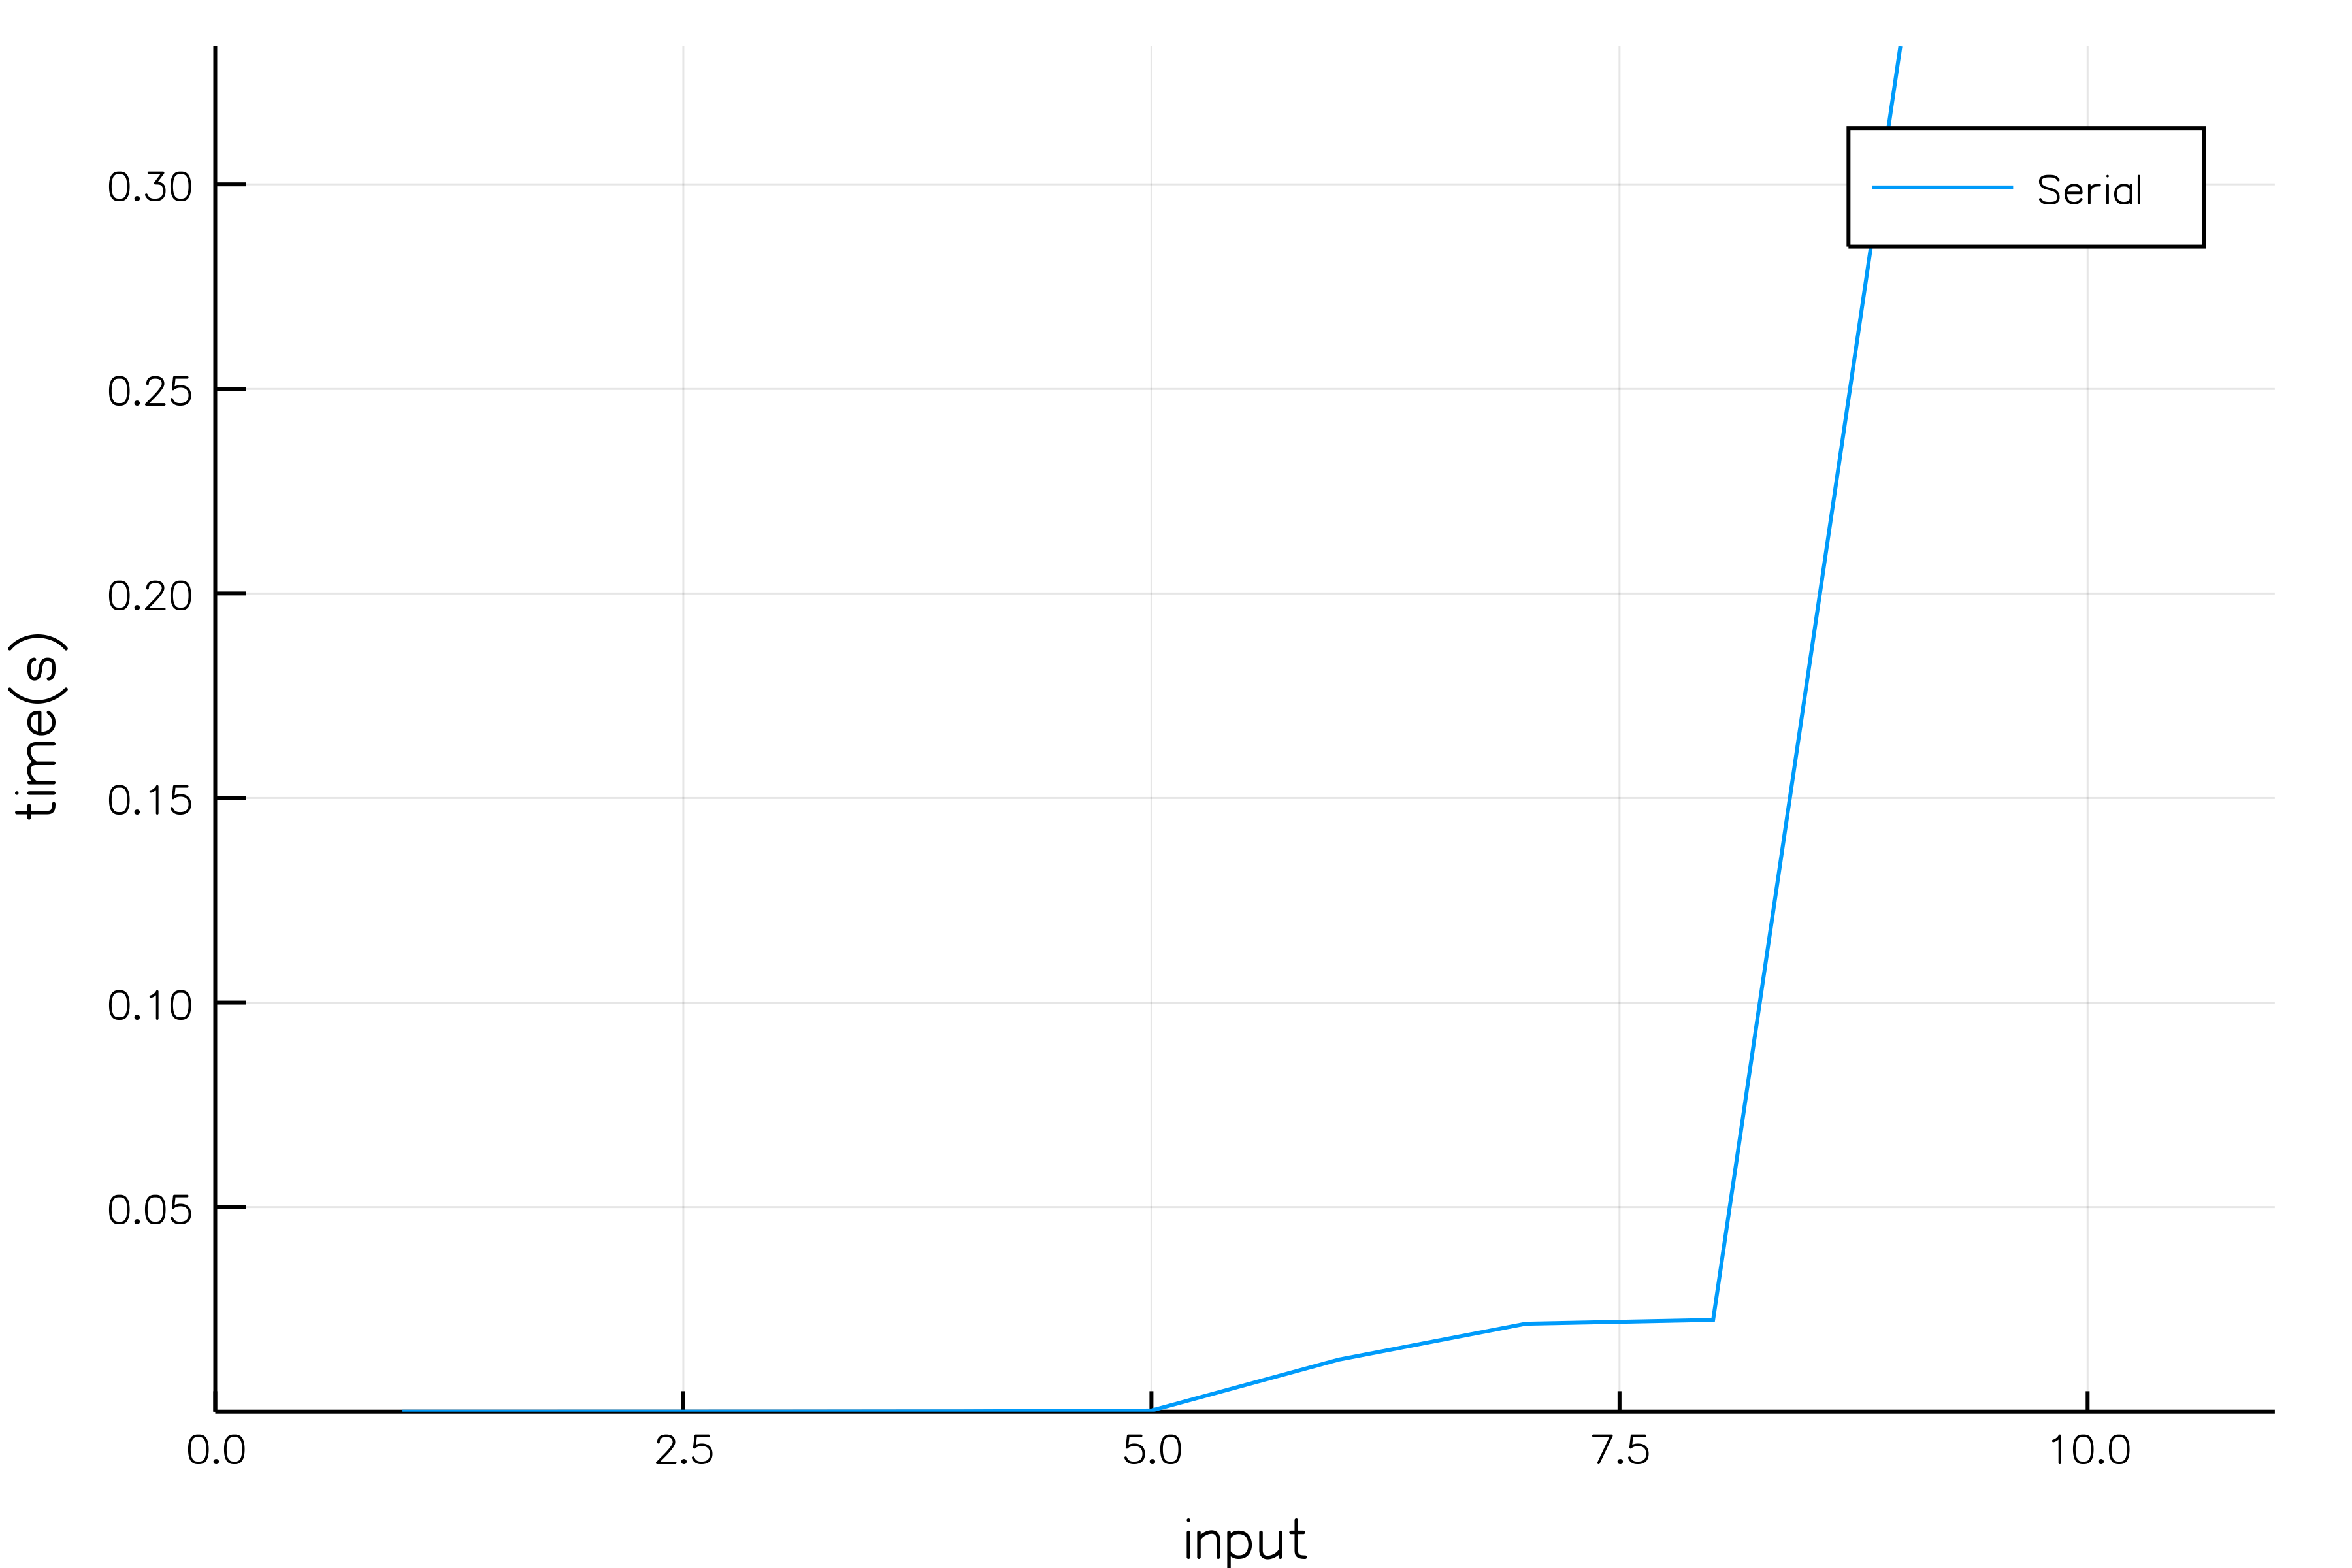
\includegraphics[width=11cm,scale=0.3]{larApplySerial.png}
\end{figure}
\begin{lstlisting}[language=Julia,format=Julia]
plot(ptimes,xlabel="input",xlims=(0,length(times)+2),{?ylabel="time(s)",label=["Parallel"])
\end{lstlisting}
\begin{figure}[ht!]
\centering
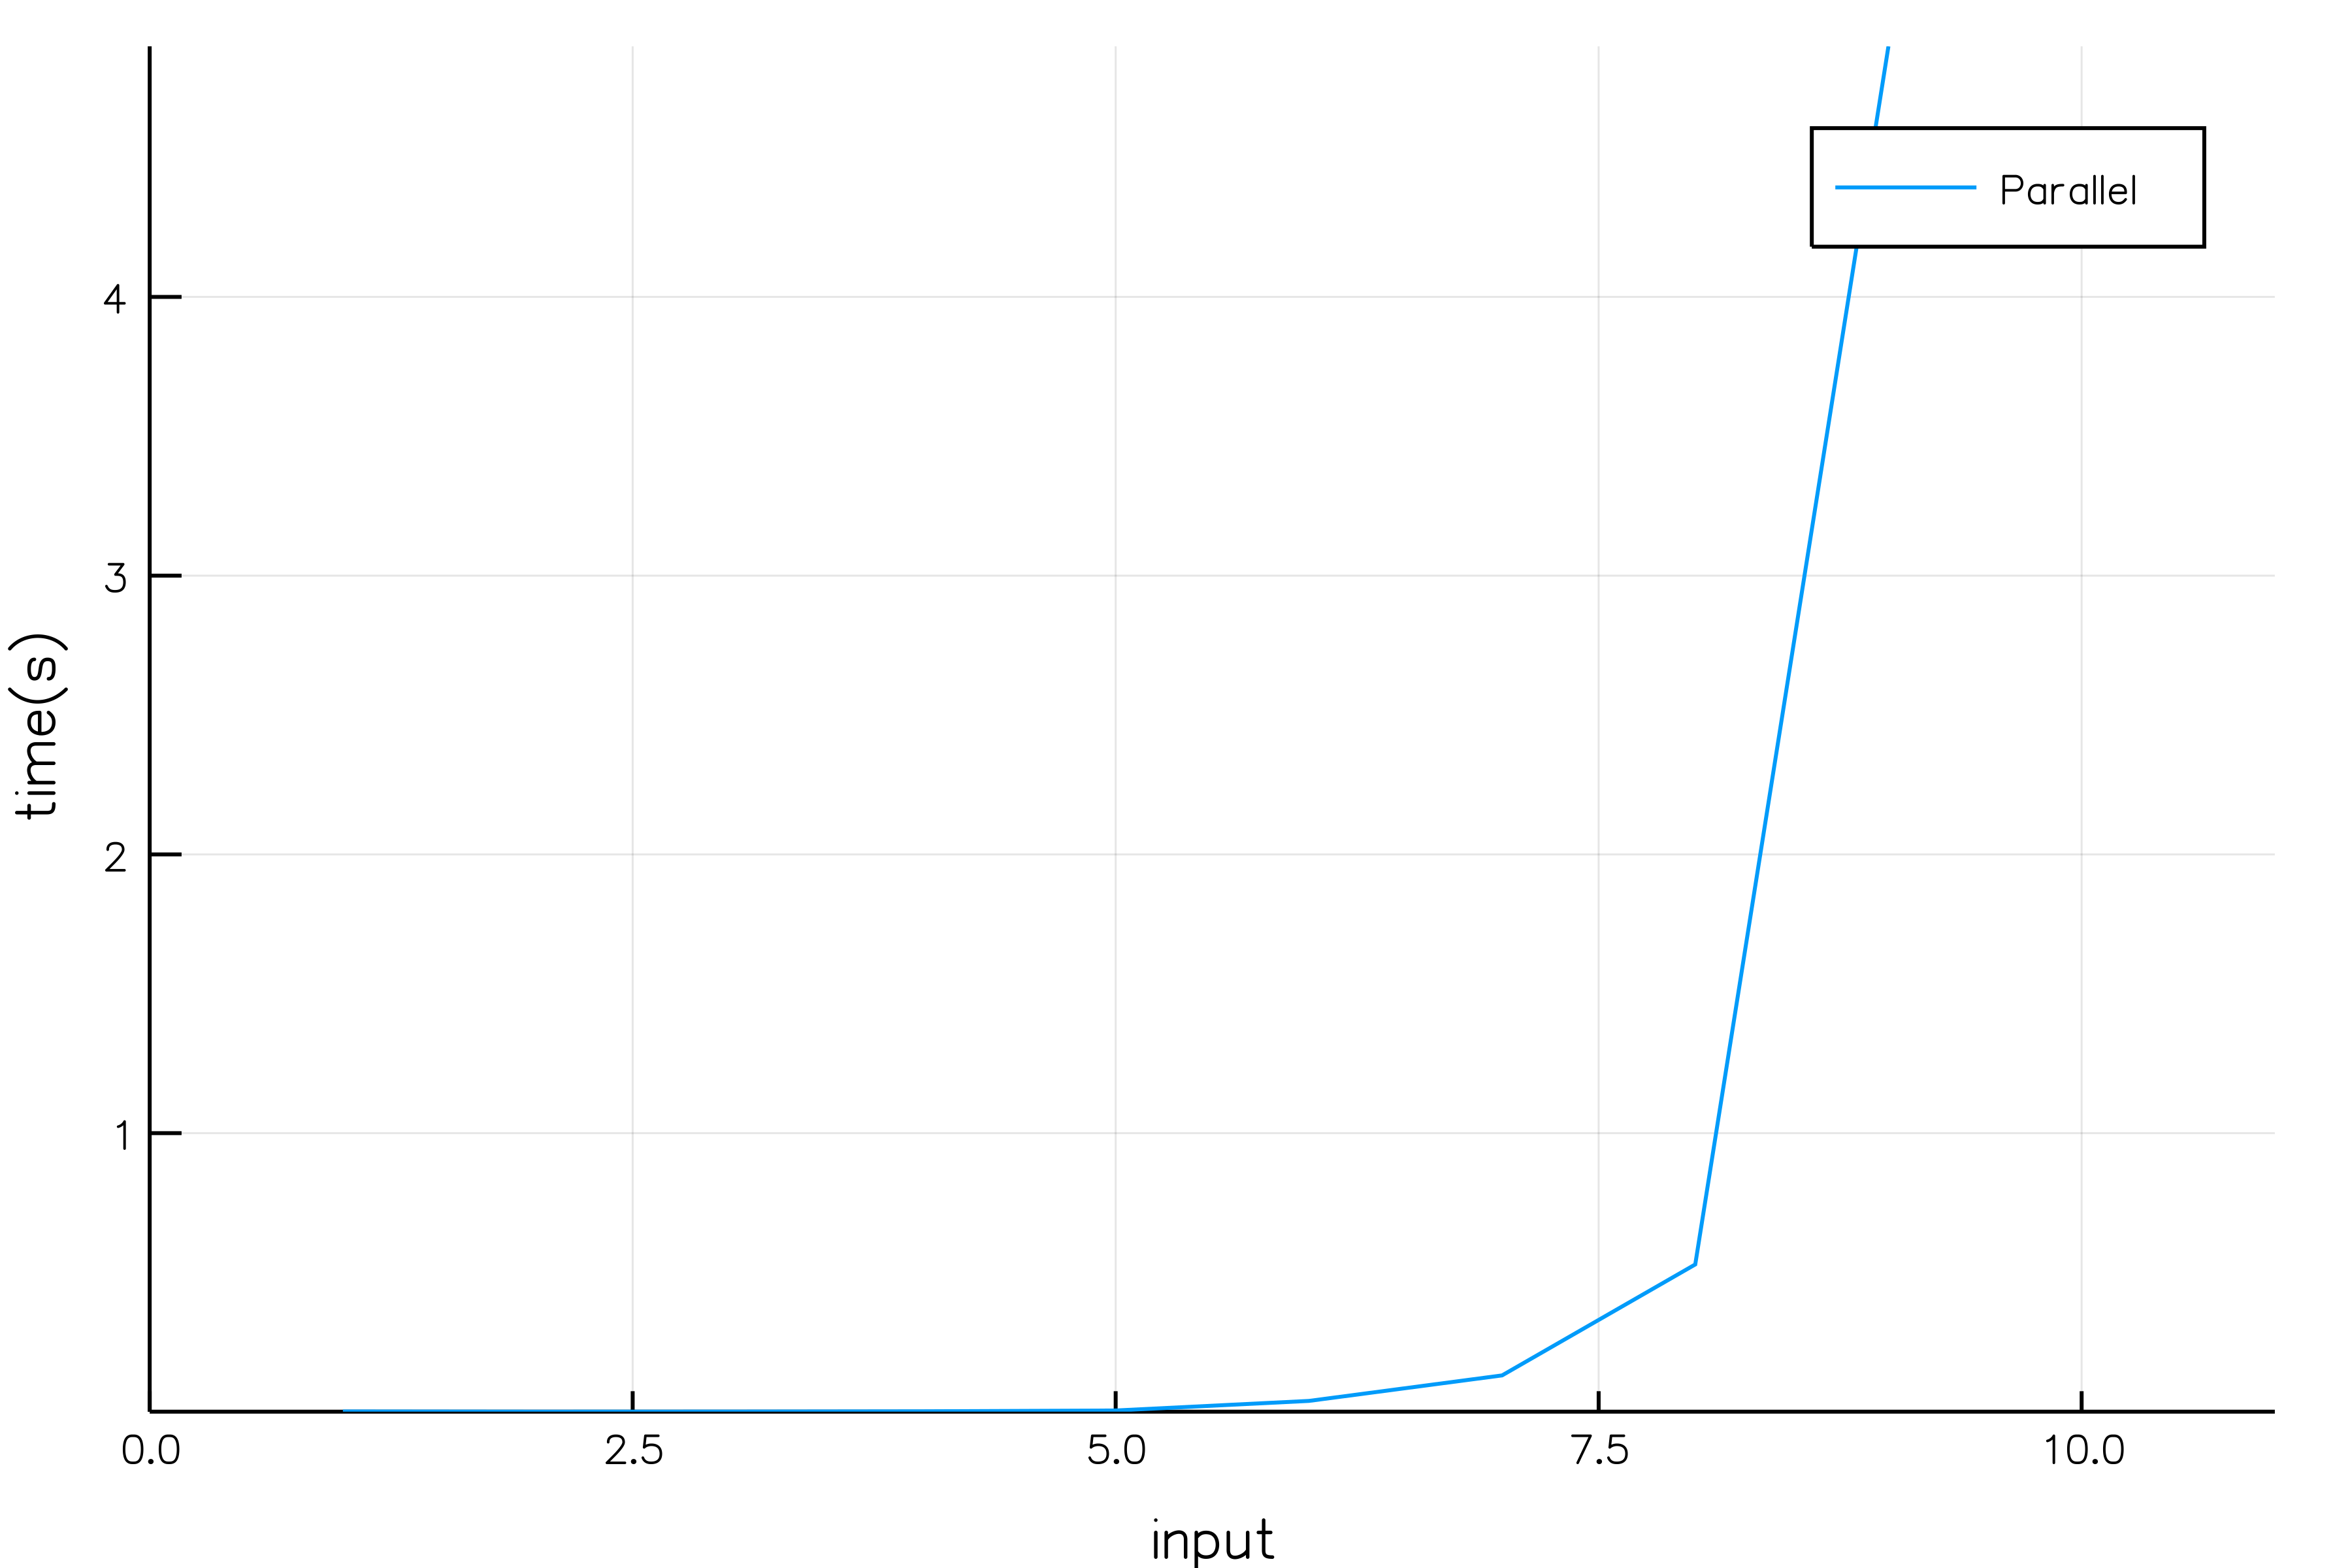
\includegraphics[width=11cm,scale=0.3]{larApplyParallel.png}
\end{figure}
\newpage
\begin{lstlisting}[language=Julia,format=Julia]
plot([times,ptimes],xlabel="input",xlims=(0,length(times)+2),{?ylabel="time(s)",label=["Serial","Parallel"])
\end{lstlisting}
\begin{figure}[ht!]
\centering
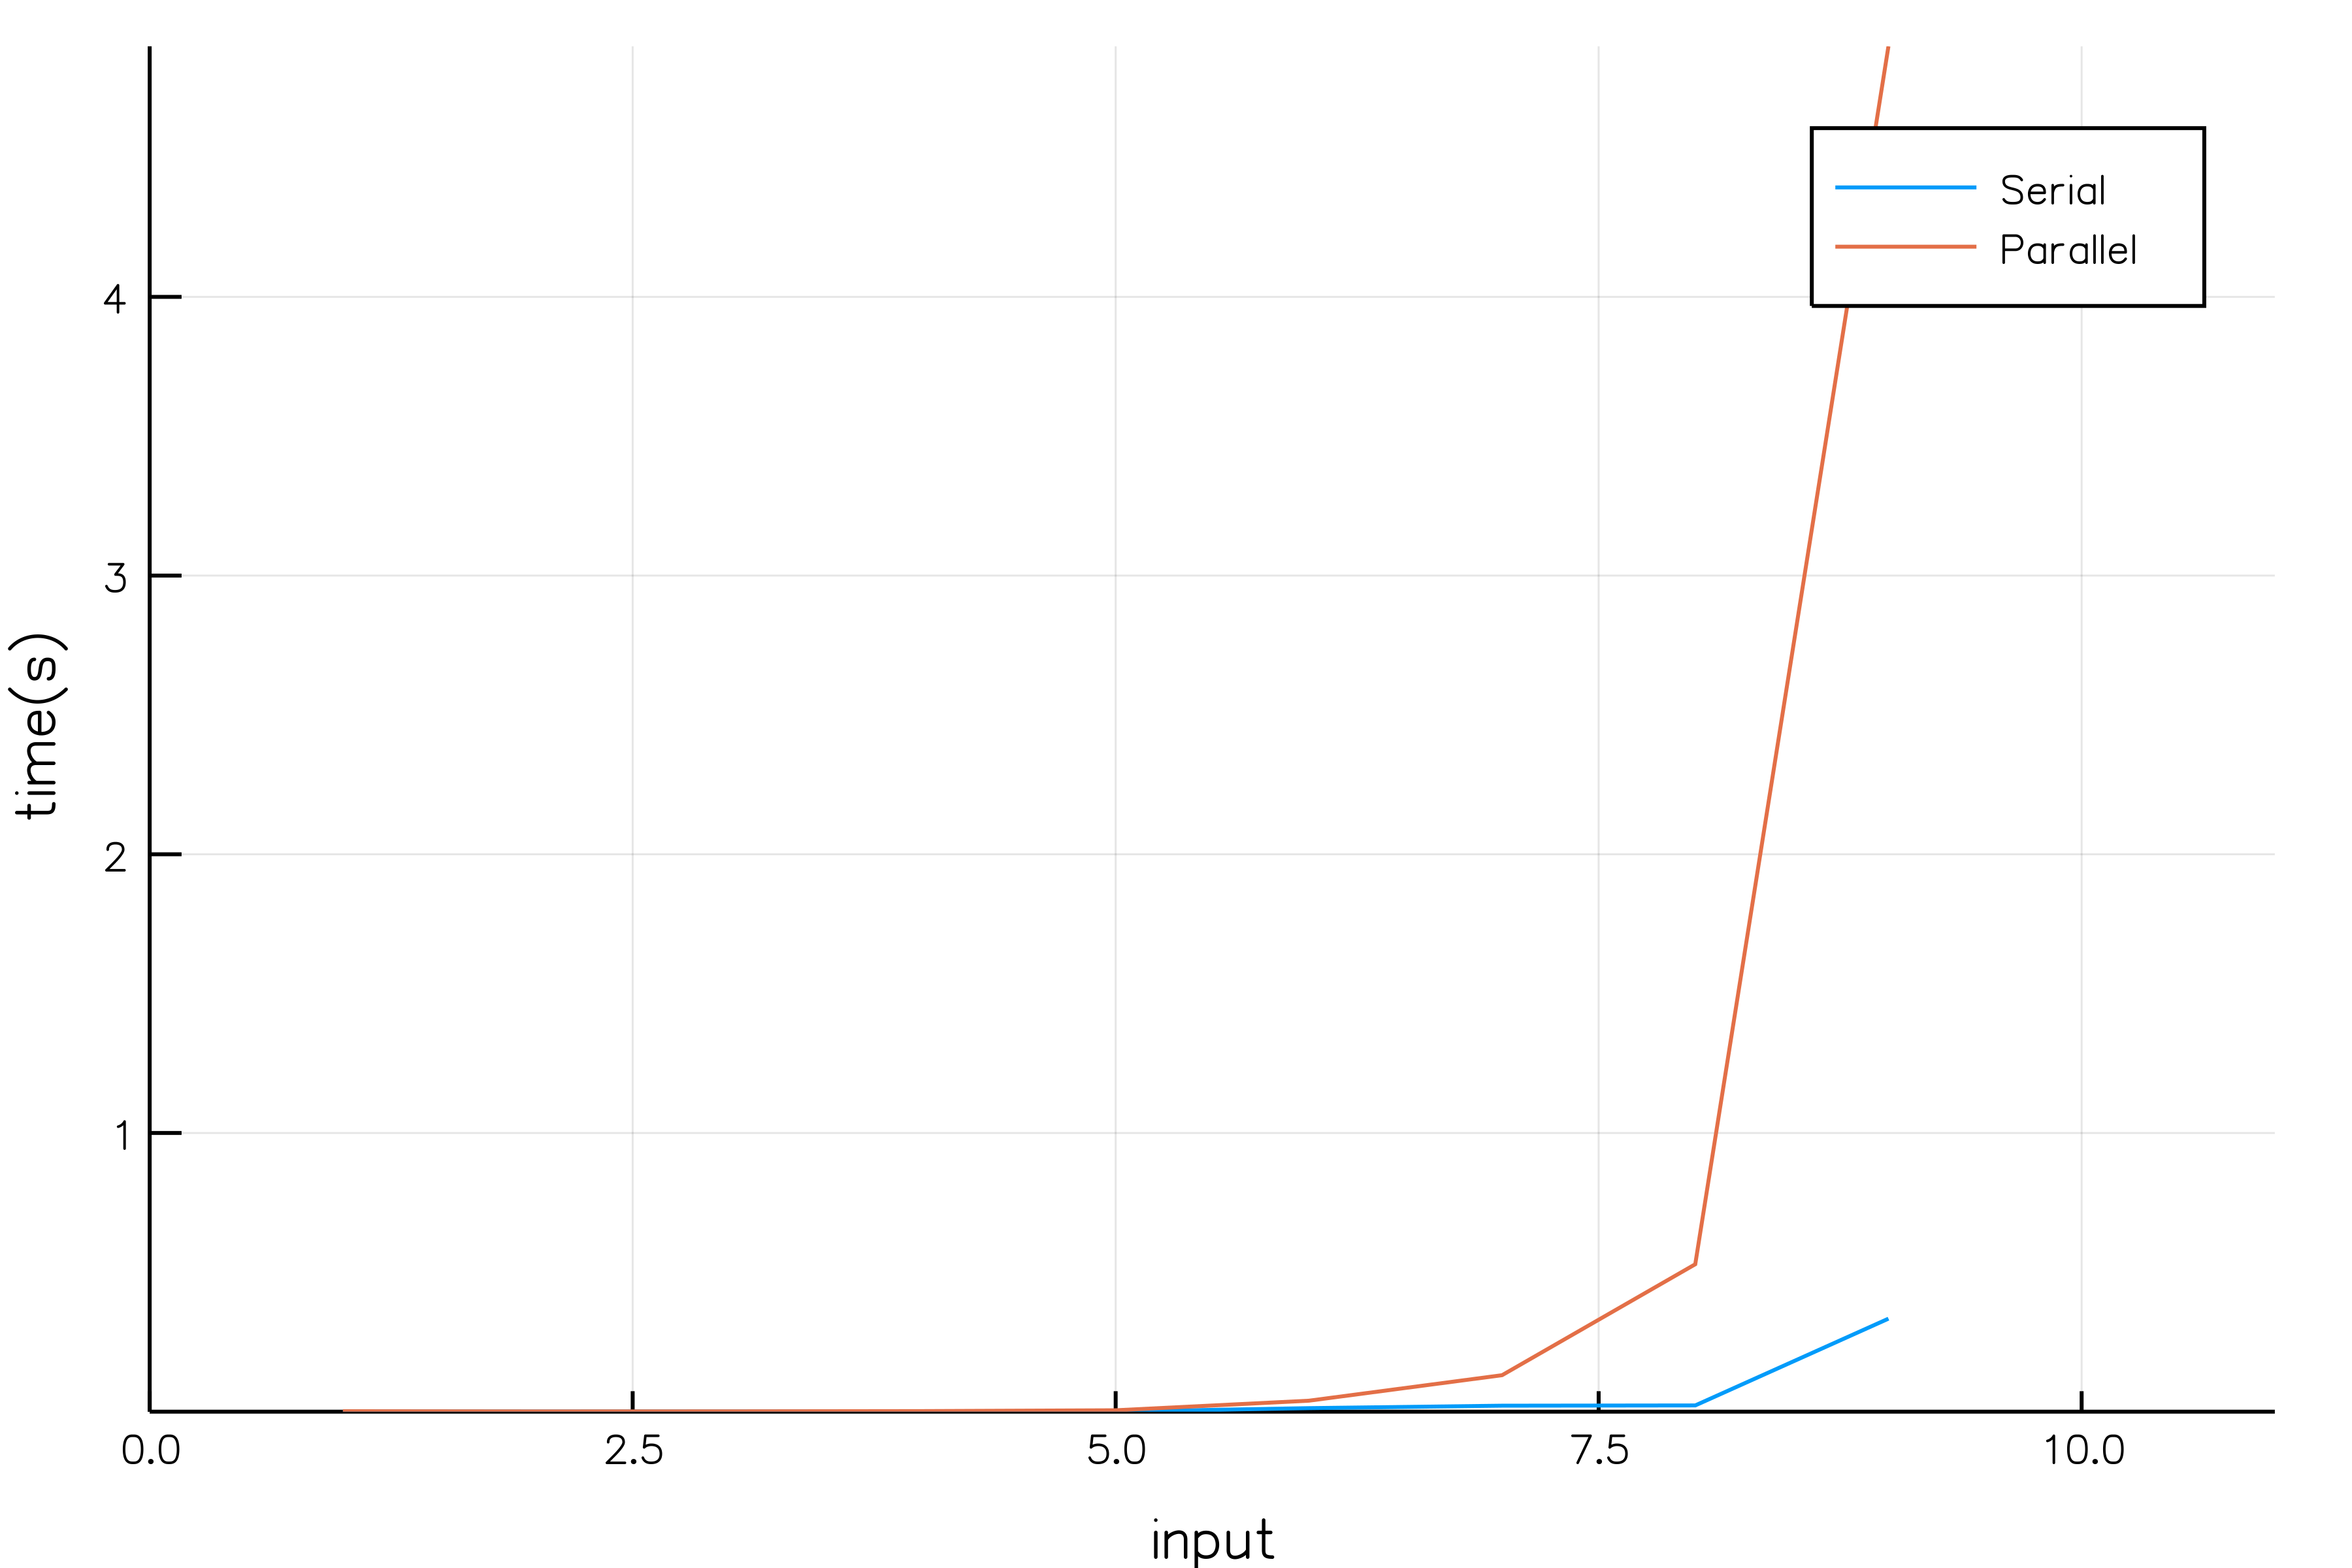
\includegraphics[width=11cm,scale=0.3]{larApplyC.png}
\end{figure}
\newpage
\subsection{box}
\subsubsection{Conversion}
\textbf{Python}
\begin{lstlisting}[language=Python,format=Julia]
def box(model):{
    if isinstance(model,Mat): return []
    elif isinstance(model,Struct):{
        dummyModel = copy.deepcopy(model)
        dummyModel.body = [term if (not isinstance(term,Struct)) {?
                        else [term.box,[[0,1]]]  for term in model.body]}
        listOfModels = evalStruct( dummyModel )
        theMin,theMax = box(listOfModels[0]) 
        for theModel in listOfModels[1:]:{
            modelMin, modelMax = box(theModel)
            theMin = [val if val<theMin[k] else theMin[k]
                     for k,val in enumerate(modelMin)]
            theMax = [val if val>theMax[k] else theMax[k]
                     for k,val in enumerate(modelMax)]}
        return [theMin,theMax]}
    elif isinstance(model,Model):{
        V = model.verts}
    elif (isinstance(model,tuple) or isinstance(model,list)) and{
          (len(model)==2 or len(model)==3):
        V = model[0]}
    coords = TRANS(V)
    theMin = [min(coord) for coord in coords]
    theMax = [max(coord) for coord in coords]
    return [theMin,theMax]
\end{lstlisting}
\textbf{julia}
\begin{lstlisting}[language=Julia,format=Julia]
function box(model){
if isa(model,Matrix){
return [ ]}
elseif isa(model,Struct){
dummyModel=deepcopy(model)
dummyModel.body=Any[ ]
for term in model.body {
if isa(term,Struct){
push!(dummyModel.body,[term.box,[0,1]])}
else{
push!(dummyModel.body,term)}
end}
end
listOfModels=evalStruct(dummyModel)
theMin,theMax=box(listOfModels[1])
for theModel in listOfModels[2:end]{
modelMin,modelMax= box(theModel)
for (k,val) in enumerate(modelMin){
if val < theMin[k]{
theMin[k]=val}
end}
end
for (k,val) in enumerate(modelMax){
if val > theMax[k]{
theMax[k]=val}
end}
end}
end
return Array[theMin,theMax]}
elseif (isa(model,Tuple)||isa(model,Array)) &&{?
(length(model)==2||length(model)==3)}
V=model[1]
theMin=[ ]
theMax=[ ]
for j in range(1,length(V[1])){
Min=V[1][j]
Max=V[1][j]
for i in range(1,length(V)){
Min=min(Min,V[i][j])
Max=max(Max,V[i][j])}
end
push!(theMin,Min)
push!(theMax,Max)}
end
return Array[theMin,theMax]}
end}
end
\end{lstlisting}
\subsubsection{Parallelization}
\begin{lstlisting}[language=Julia,format=Julia]
function pbox(model){
	if isa(model,Matrix){
		return [ ]}
	elseif isa(model,pStruct){
		dummyModel=deepcopy(model)
		dummyModel.body=Any[ ]
		@sync for term in model.body{
			if isa(term,pStruct){
				push!(dummyModel.body,[term.box,[0,1]])}
			else{
				push!(dummyModel.body,term)}
			end}
		end
		listOfModels=pevalStruct(dummyModel)
		theMin,theMax=pbox(listOfModels[1])
		@sync for theModel in listOfModels[2:end]{
			modelMin,modelMax= pbox(theModel)
		       @async begin{
		       for (k,val) in enumerate(modelMin){
				if (val < theMin[k]){
					theMin[k]=val}
				end}
			end
			for (k,val) in enumerate(modelMax){
			    if (val > theMax[k]){
			    	theMax[k]=val}
			     end}
			end}
			end}			
		end
		return Array[theMin,theMax]}
	elseif (isa(model,Tuple) ||isa(model,Array))&& {?
	(length(model)==2 || length(model)==3)}
		V=model[1]
	theMin=[ ]
	theMax=[ ]
		@sync for j in range(1,length(V[1])){
			Min=V[1][j]
			Max=V[1][j]
			for i in range(1,length(V)){
				Min=min(Min,V[i][j])
				Max=max(Max,V[i][j])}
			end
			@async begin{
			push!(theMin,Min)
			push!(theMax,Max)}
			end}
		end
	return Array[theMin,theMax]}
	end}
end
\end{lstlisting}
\subsubsection{Unit-Test}
These Unit-Test can be runned after the definition of the Struct type on the section \ref{Struct}
\begin{lstlisting}[language=Julia]
square=([[0,0],[0,1],[1,0],[1,1]],[[0,1,2,3]])
cubes=([[0,0,0],[0,0,1],[0,1,0],[0,1,1],[1,0,0],[1,0,1],[1,1,0],
       [1,1,1]],[[[0],[1],[2],[3],[4],[5],[6],[7]],[[0,1],[2,3],[4,5],
       [6,7],[0,2],[1,3],[4,6],[5,7],[0,4],[1,5],[2,6],[3,7]],
       [[0,1,2,3],[4,5,6,7],[0,1,4,5],[2,3,6,7],[0,2,4,6],
       [1,3,5,7]],[[0,1,2,3,4,5,6,7]]])

@testset "box Tests" begin
  @testset "box Tests 2D" begin
    @test typeof(box(square))==Array{Array,1}
    @test length(box(square))==2
    @test length(box(square)[1])==2
  end
  @testset "box Tests 3D" begin
    @test typeof(box(cubes))==Array{Array,1}
    @test length(box(cubes))==2
    @test length(box(cubes)[1])==3
  end
end

square=([[0,0],[0,1],[1,0],[1,1]],[[0,1,2,3]])
cubes=([[0,0,0],[0,0,1],[0,1,0],[0,1,1],[1,0,0],[1,0,1],[1,1,0],
       [1,1,1]],[[[0],[1],[2],[3],[4],[5],[6],[7]],[[0,1],[2,3],[4,5],
       [6,7],[0,2],[1,3],[4,6],[5,7],[0,4],[1,5],[2,6],[3,7]],
       [[0,1,2,3],[4,5,6,7],[0,1,4,5],[2,3,6,7],[0,2,4,6],
       [1,3,5,7]],[[0,1,2,3,4,5,6,7]]])

@testset "pbox Tests" begin
	@testset "pbox Tests 2D" begin
		@test typeof(pbox(square))==Array{Array,1}
		@test length(pbox(square))==2
		@test length(pbox(square)[1])==2
	end
	@testset "pbox Tests 3D" begin
		@test typeof(pbox(cubes))==Array{Array,1}
		@test length(pbox(cubes))==2
		@test length(pbox(cubes)[1])==3
	end
end
\end{lstlisting}
\subsubsection{Results}
\textbf{Tesla}
\begin{lstlisting}[language=Julia]
input=[1,10,50,10^2,5*10^2,10^3,5*10^3,10^4,5*10^4,10^5,5*10^5,10^6]
function timeFstruct(f::Function,pf::Function,model,input)
	t=Array{Float64}(length(input))
	pt=Array{Float64}(length(input))
	for i in range(1,length(input))
	    structo=addn2D(input[i],model)
	    pstructo=pStruct(structo.body)
	    f(structo)
	    pf(pstructo)
	    t[i]=@elapsed f(structo)
	    pt[i]=@elapsed pf(pstructo)
	end
	return t,pt
end

y,yp=timeFstruct(box,pbox,square,input)
p=plot(y,xaxis=''input'',yaxis=''time'',xlims=(0,length(input)+1),
       ylims=(0,maximum(y)+0.5), label=[''Serial''],lw=2)
\end{lstlisting}
\begin{figure}[ht!]
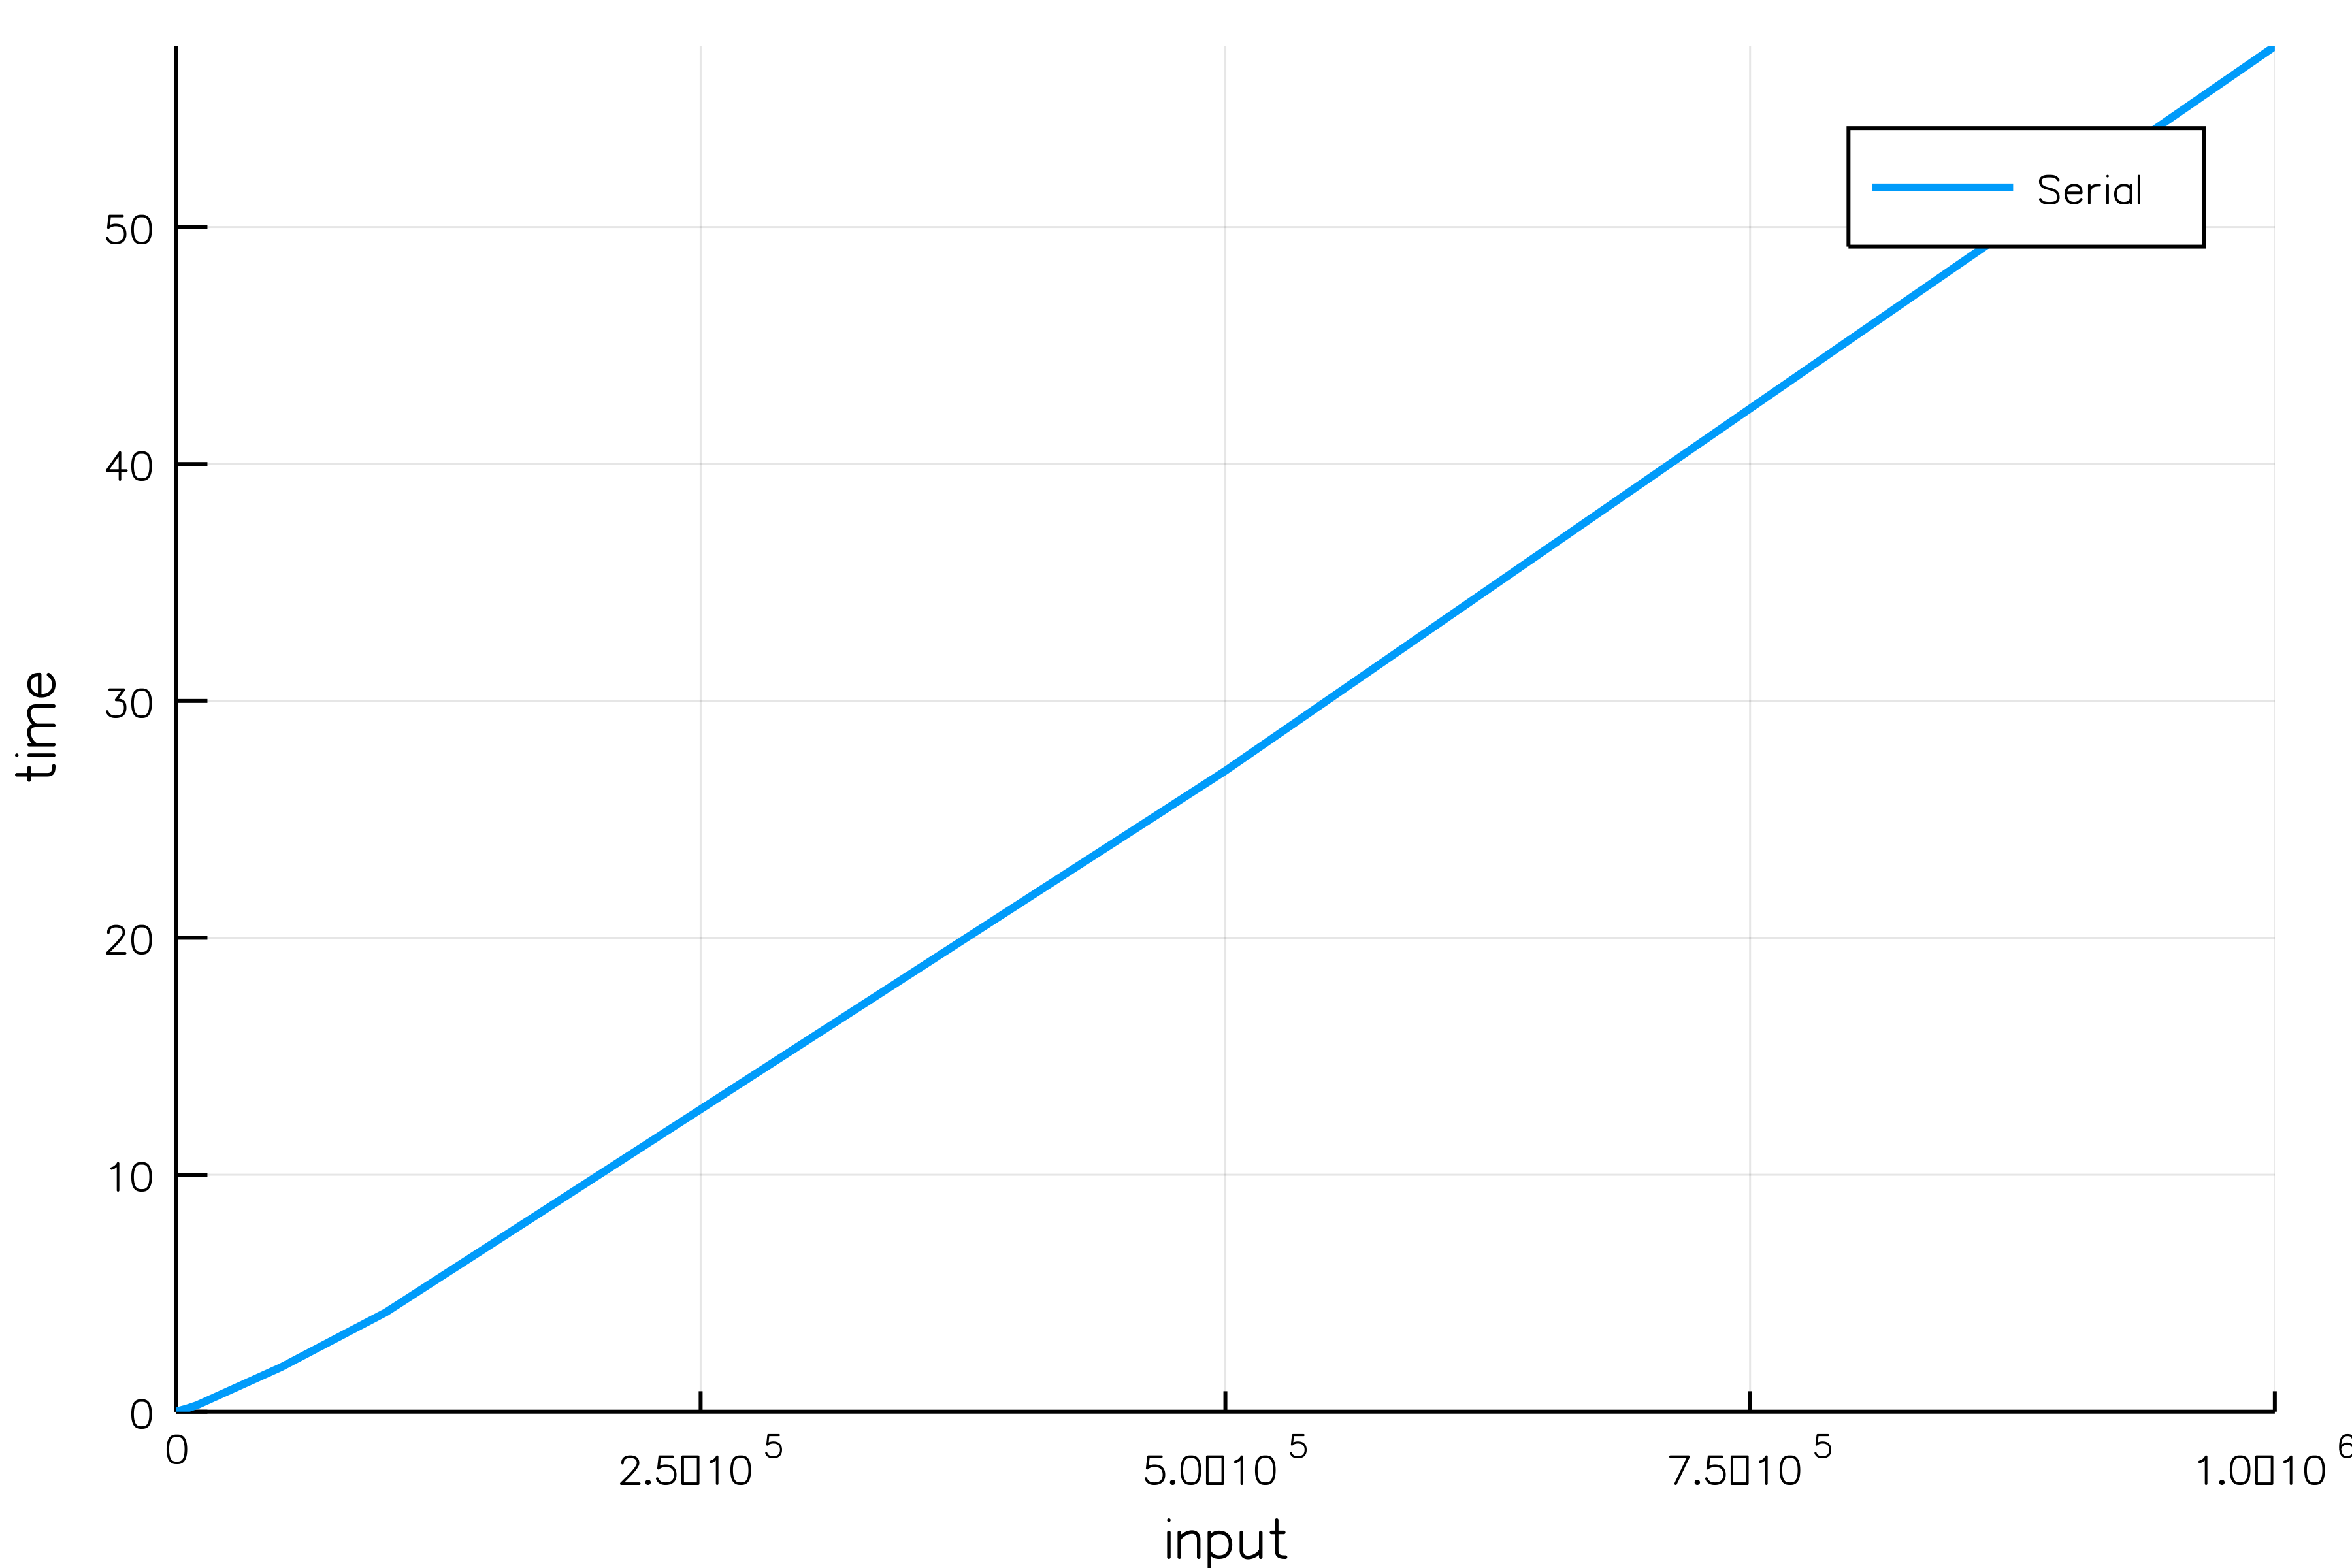
\includegraphics[width=11cm,scale=0.3]{box.png}
\end{figure}
\newpage
\begin{verbatim}
pp=plot(yp,xaxis=''input'',yaxis=''time'',xlims=(0,length(input)+1),
       ylims=(0,maximum(y)+0.5),label=[''Parallel''],lw=2)
\end{verbatim}
\begin{figure}[ht!]
\centering
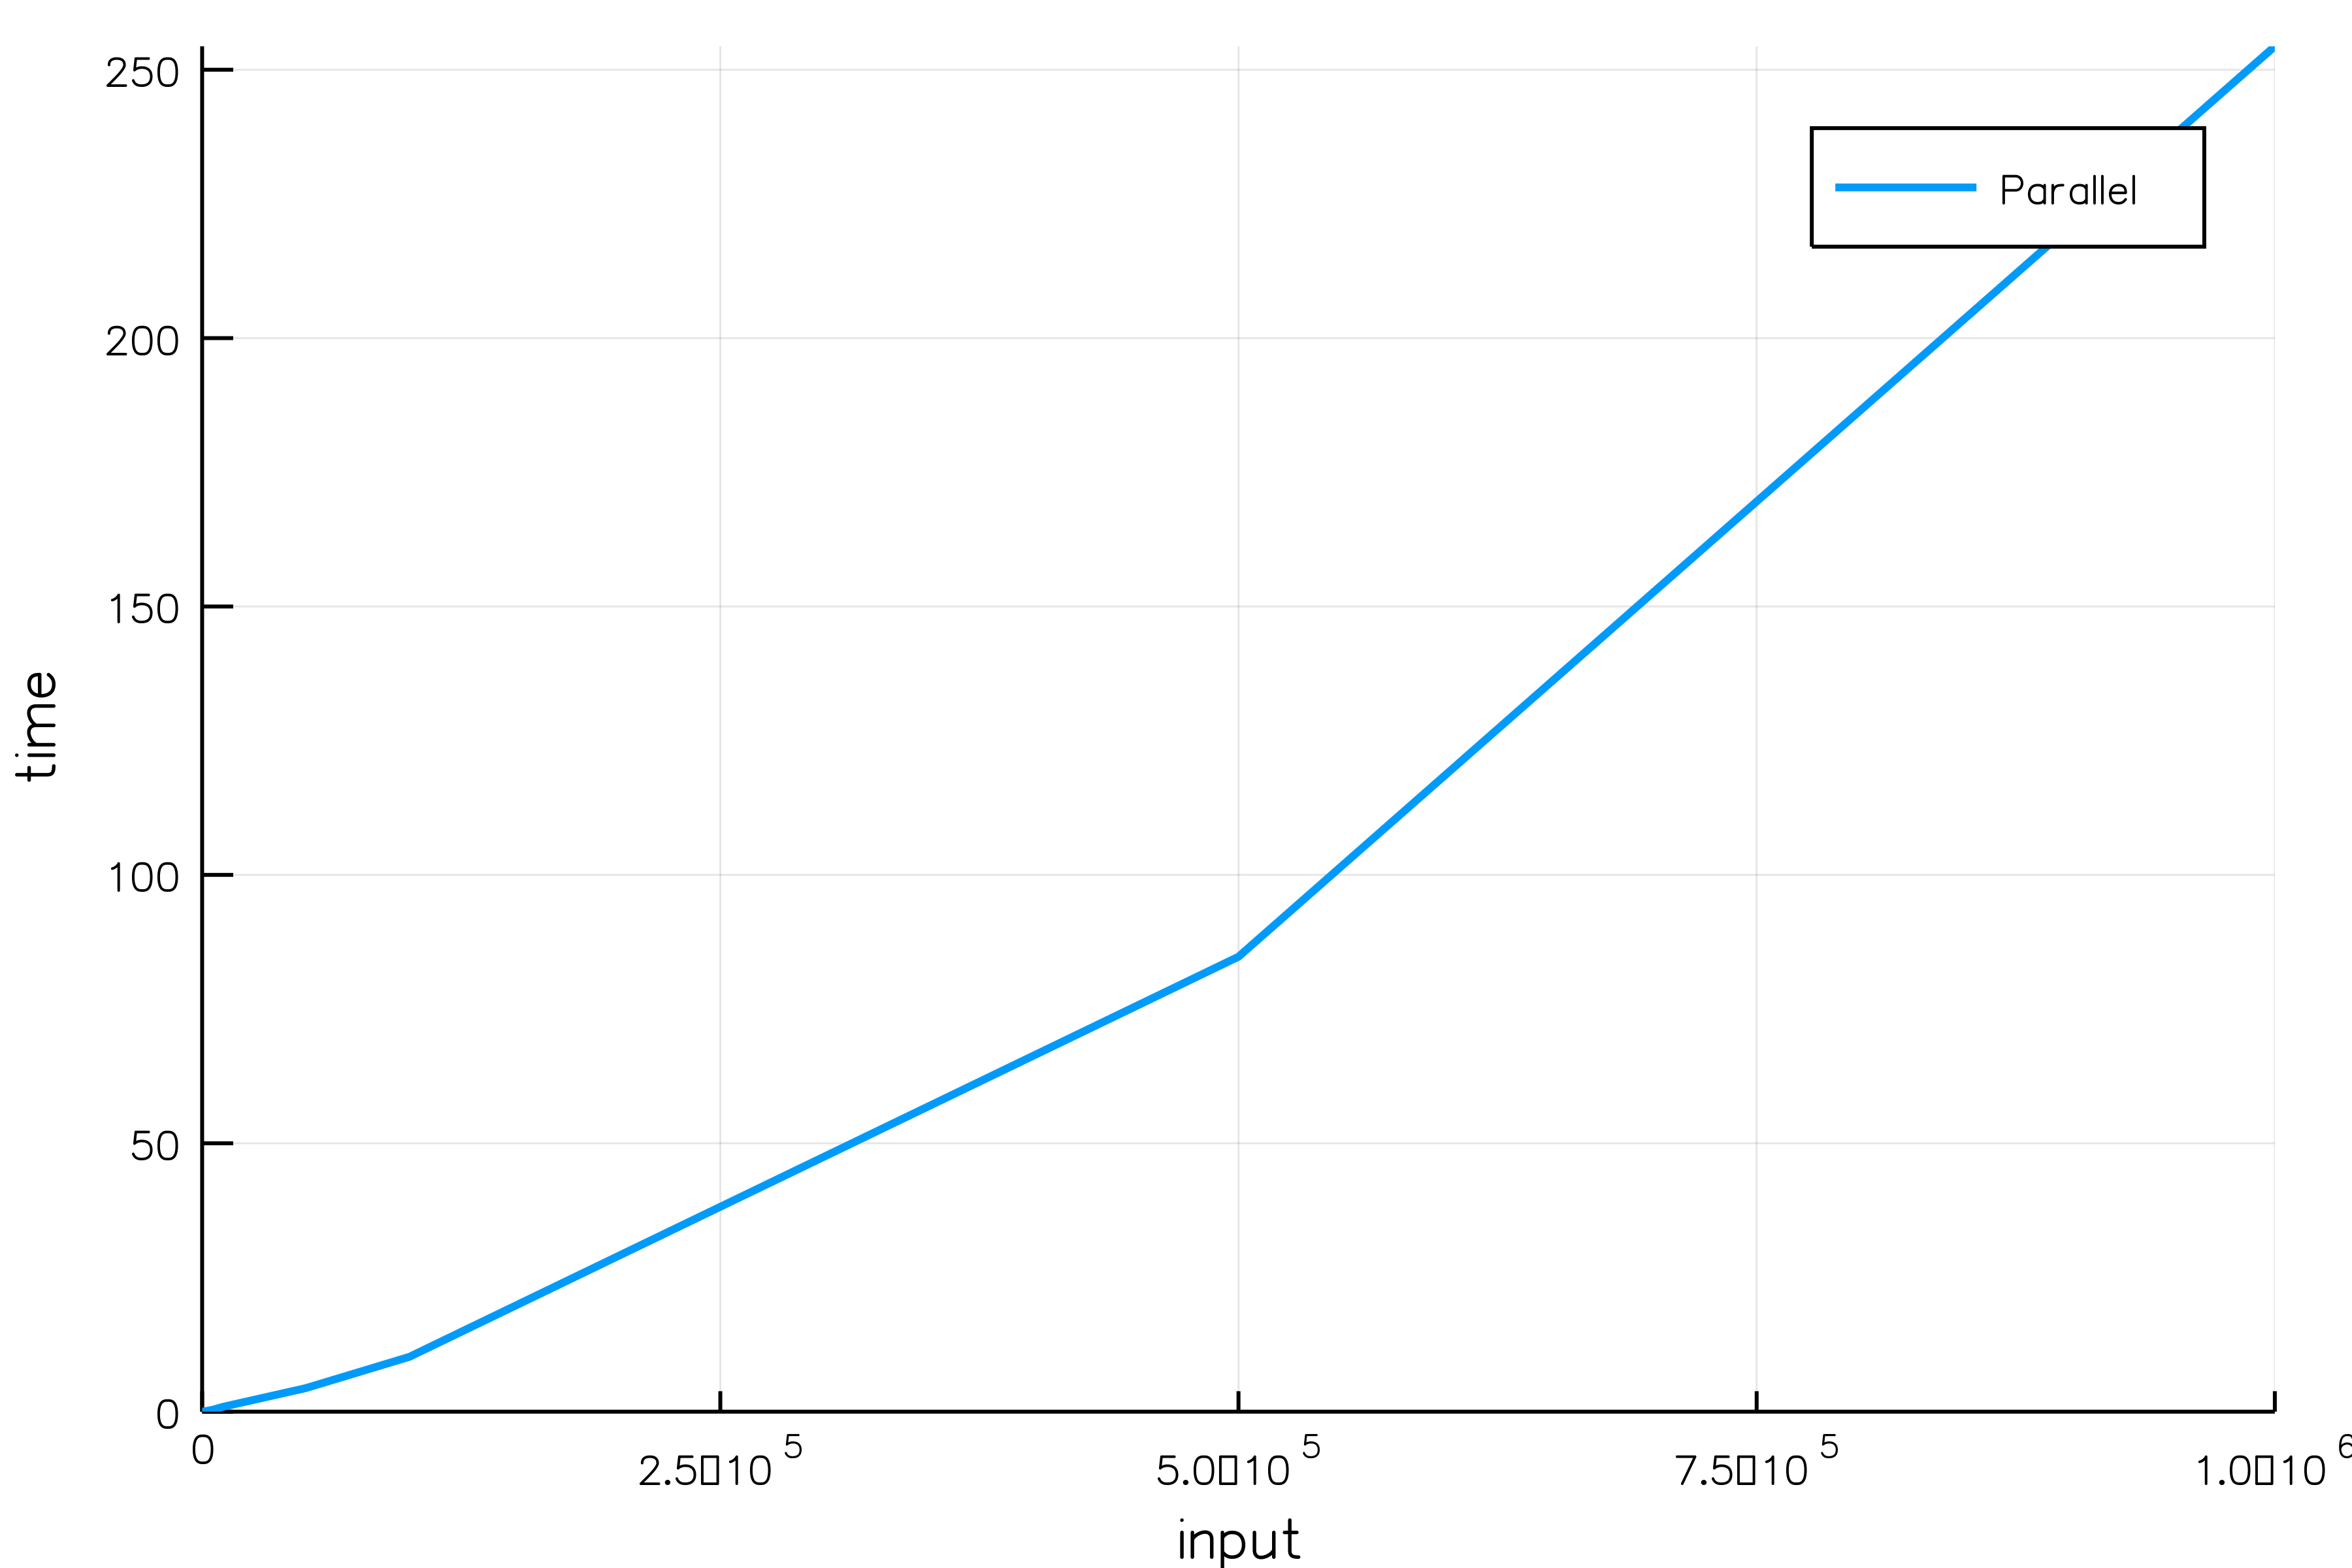
\includegraphics[width=11cm,scale=0.3]{pbox.png}
\end{figure}
\begin{verbatim}
yc=[y,yp]
pc=plot(yc,label=["Serial" "Parallel"])
\end{verbatim}
\begin{figure}[ht!]
\centering
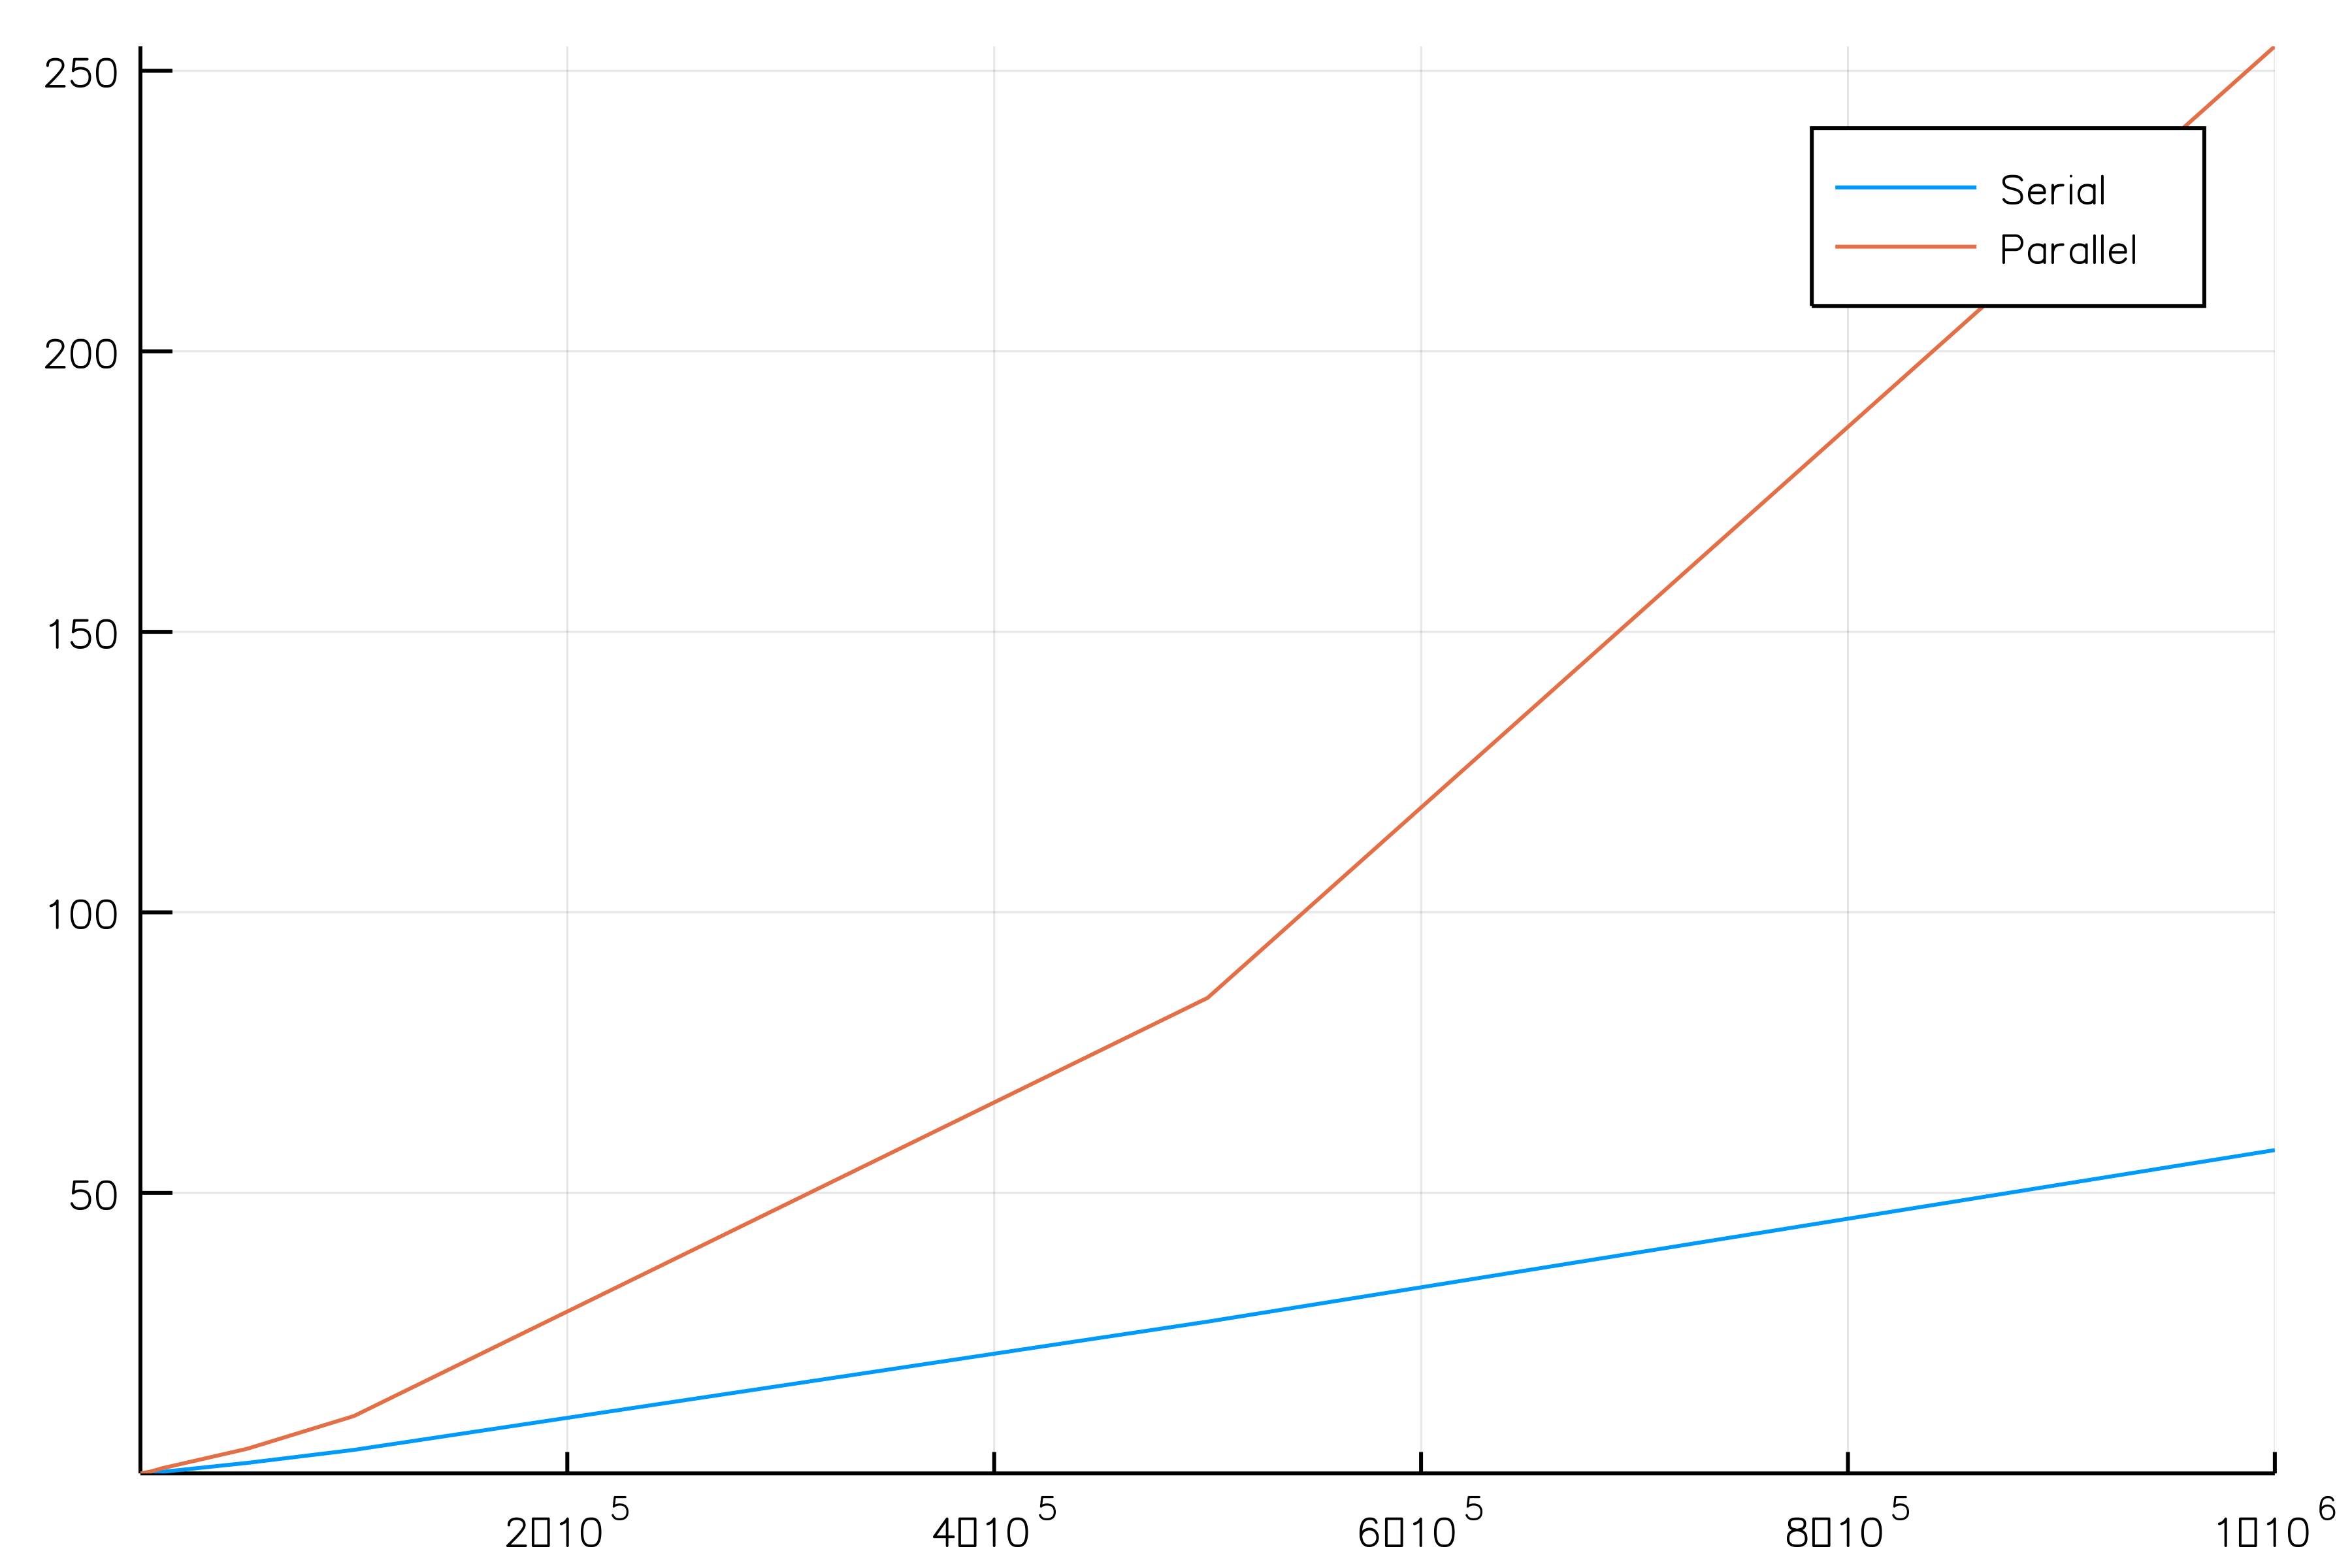
\includegraphics[width=11cm,scale=0.5]{compbox.png}
\end{figure}
\newpage
\textbf{PC}
\begin{lstlisting}[language=Julia,format=Julia]
times=[ ]
ptimes=[ ]
input=[ ]
for i in range(1,length(l)){
    push!(input,Struct([repeat([l[i]],outer=i)...]))}
end
for i in range(1,length(input)){
    append!(times,Time(box,input[i]))}
end
for i in range(1,length(input)){
    append!(ptimes,Time(pbox,input[i]))}
end

plot(times,xlabel="input",xlims=(0,length(times)+2),{?ylabel="time(s)",label=["Serial"])
\end{lstlisting}
\begin{figure}[ht!]
\centering
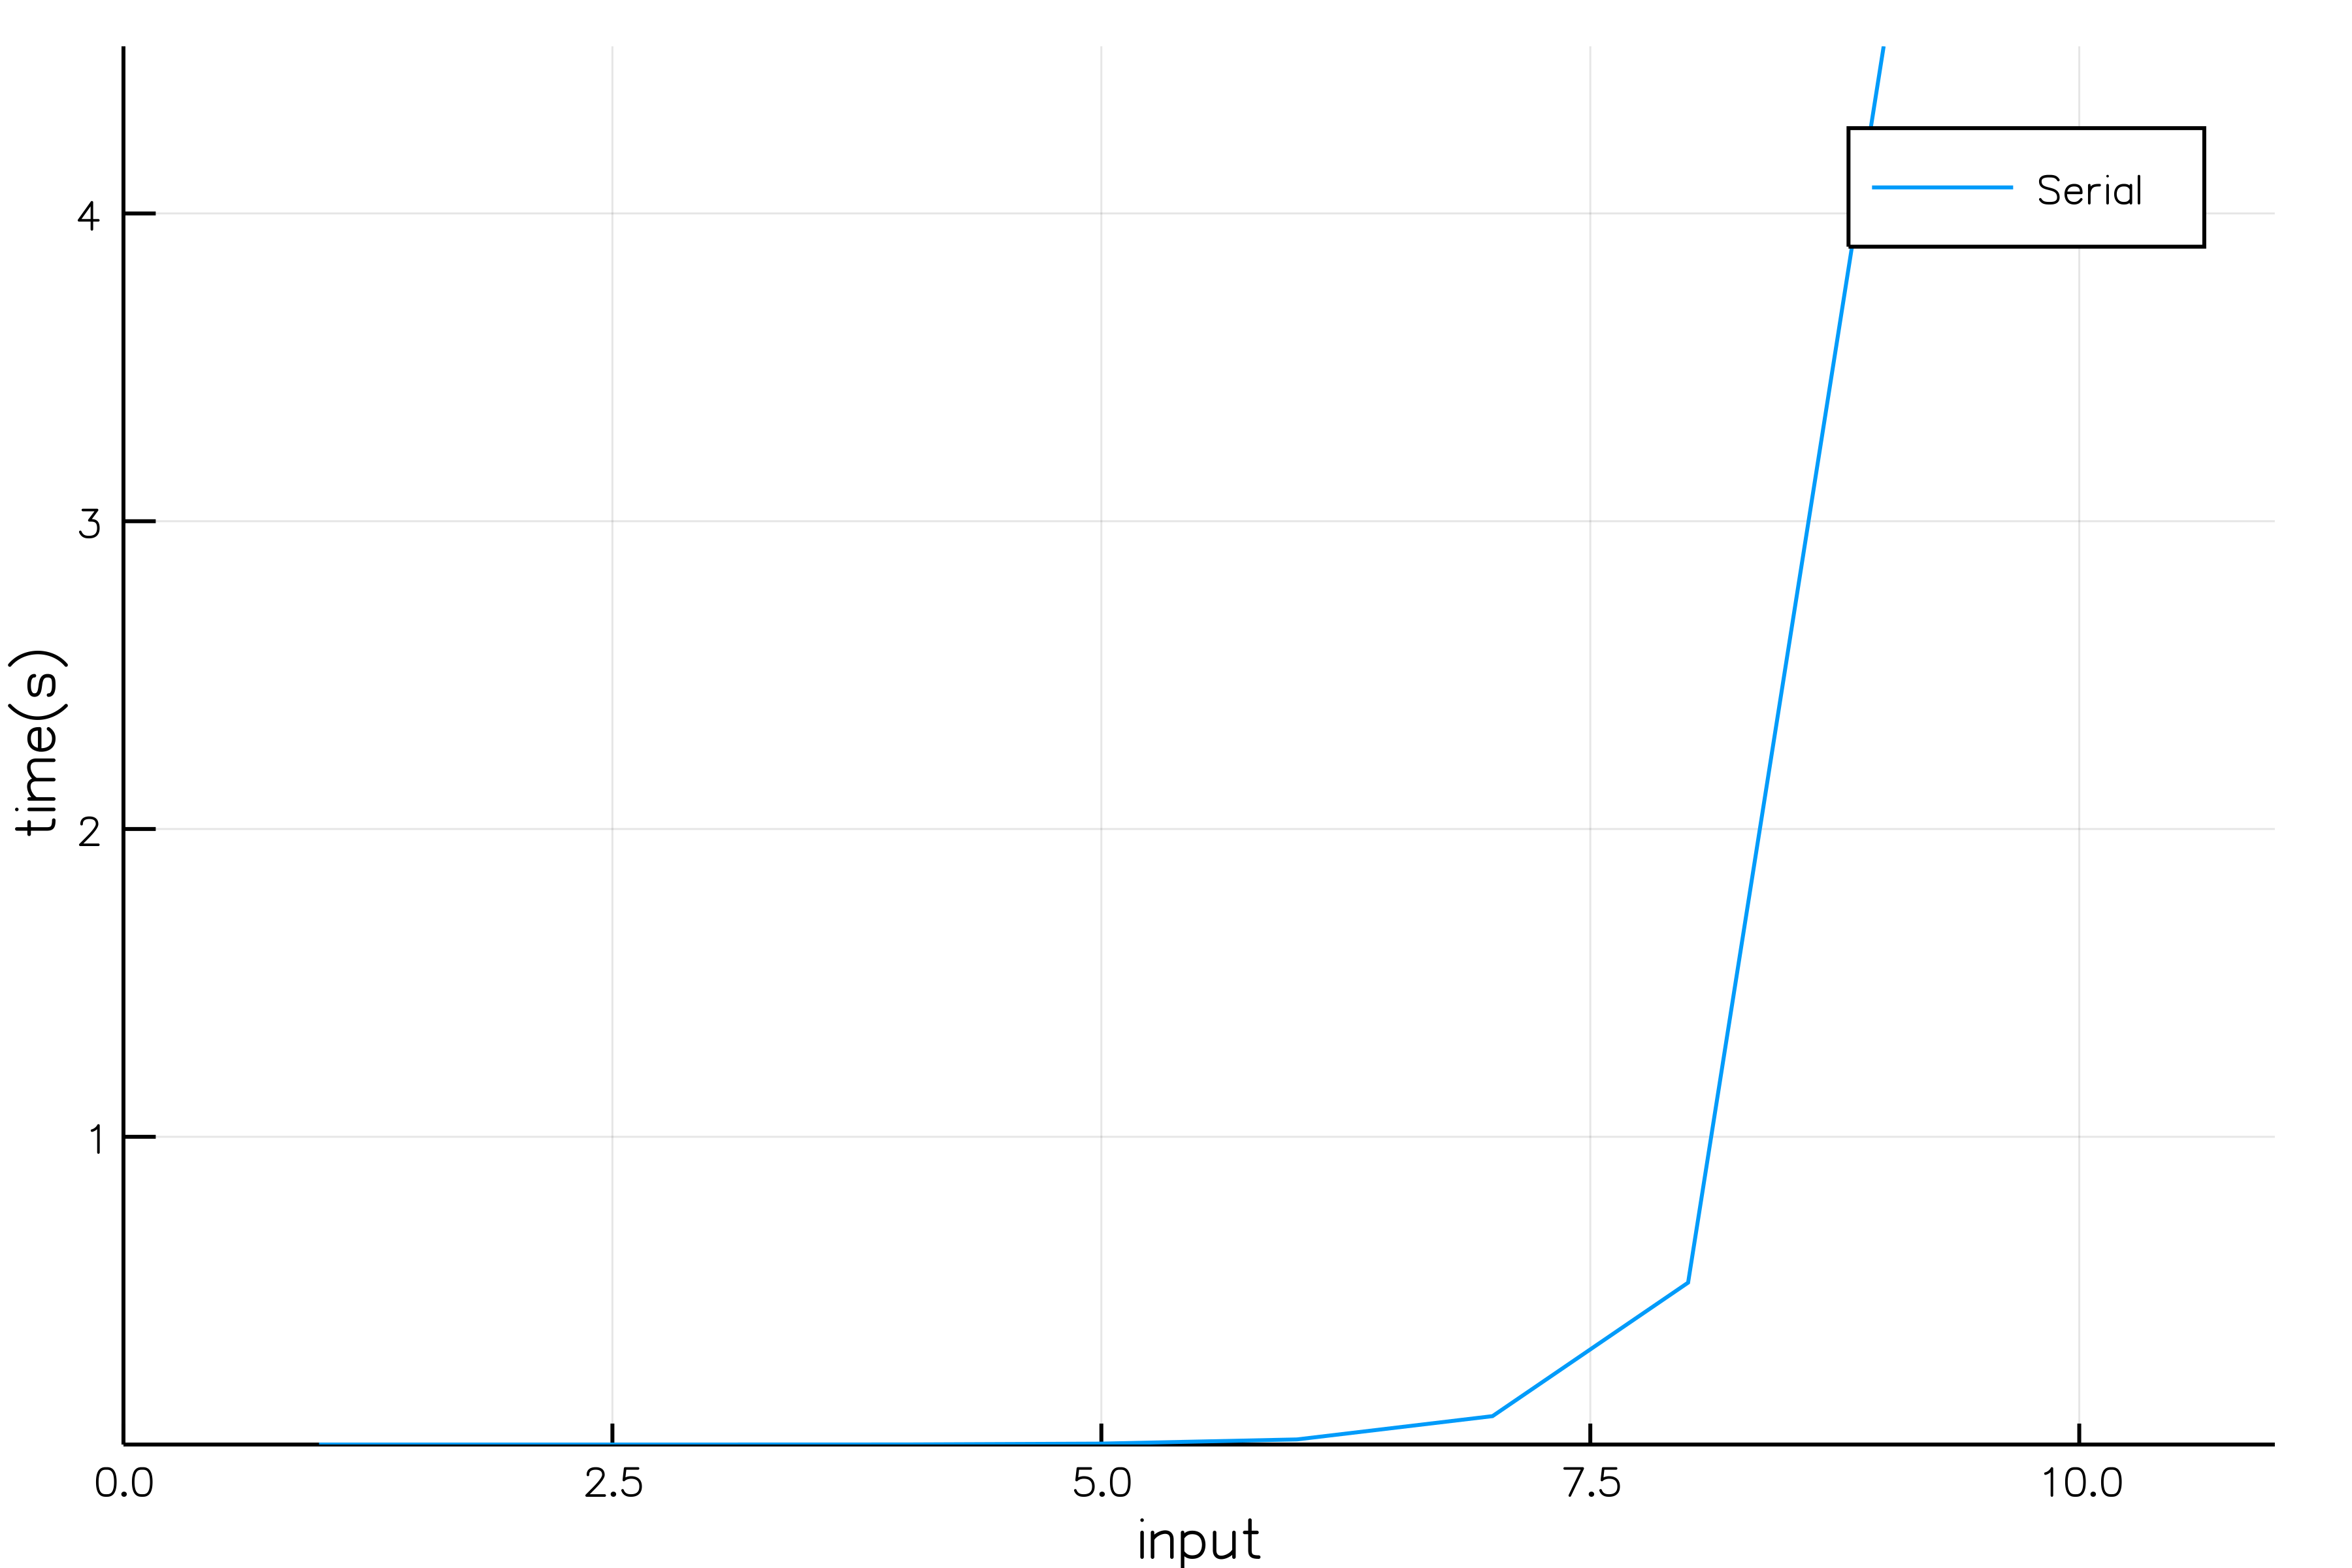
\includegraphics[width=11cm,scale=0.3]{boxSerial.png}
\end{figure}
\newpage
\begin{lstlisting}[language=Julia,format=Julia]
plot(ptimes,xlabel="input",xlims=(0,length(times)+2),{?ylabel="time(s)",label=["Parallel"])
\end{lstlisting}
\begin{figure}[ht!]
\centering
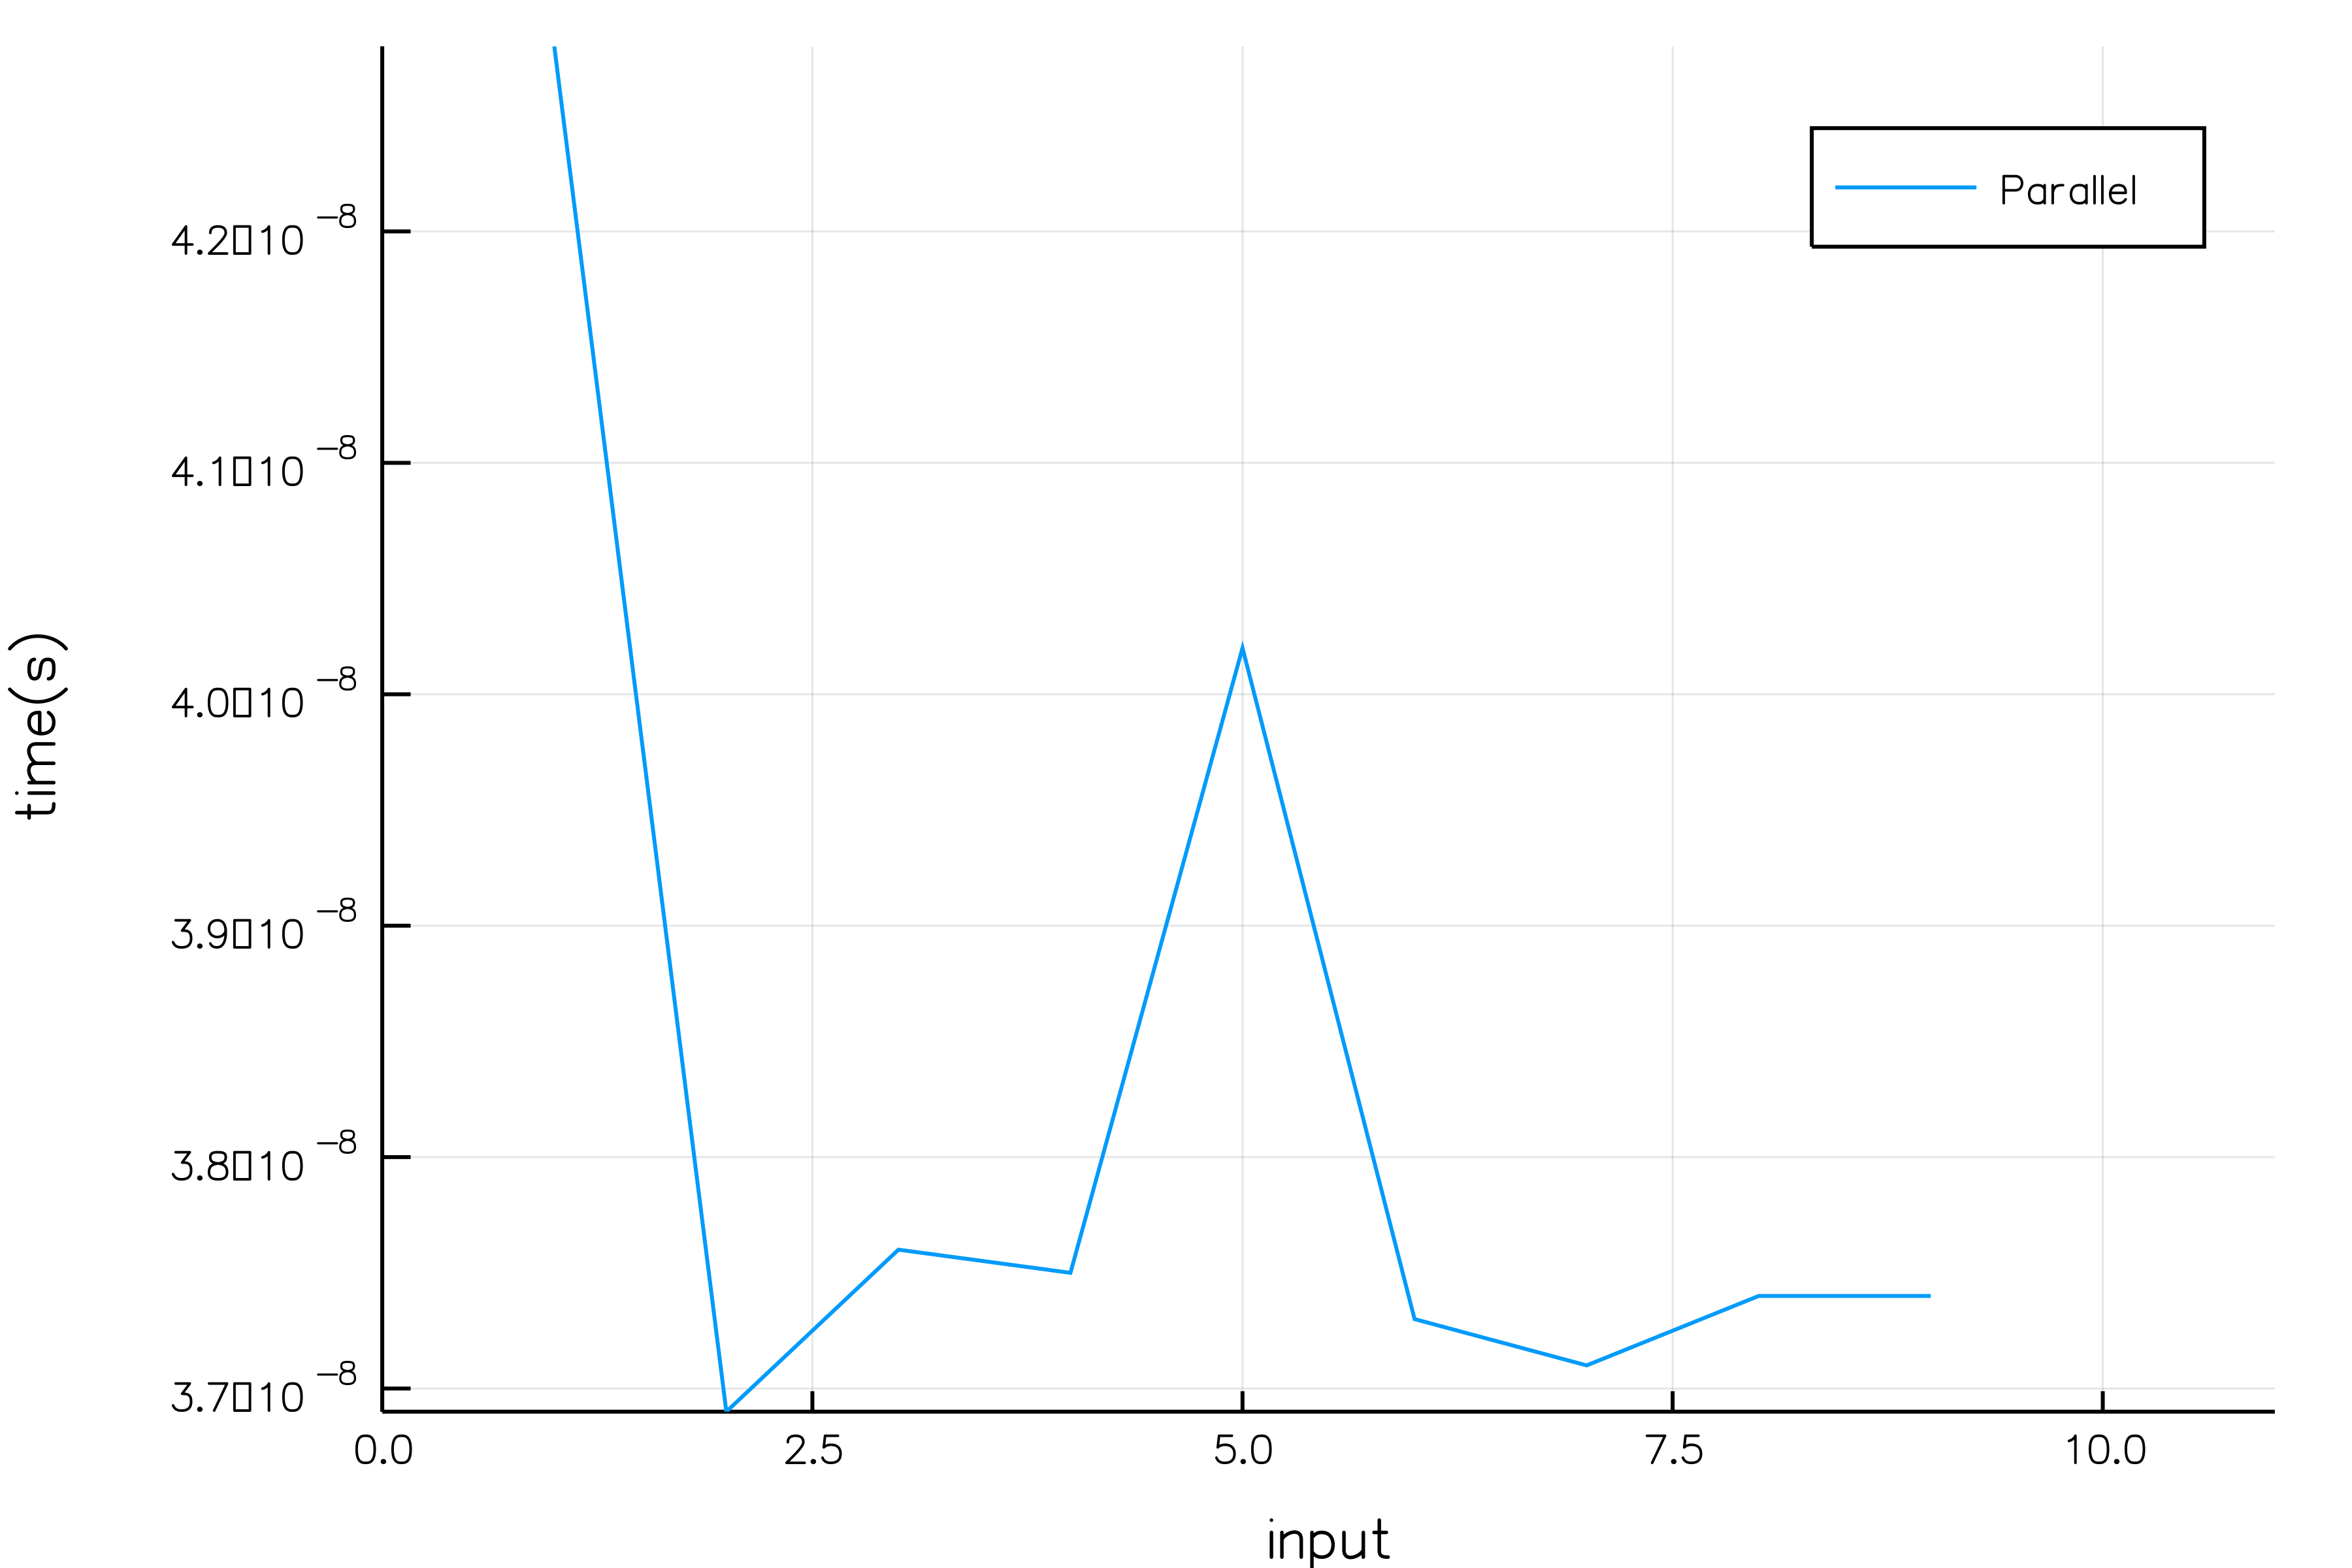
\includegraphics[width=11cm,scale=0.3]{boxParallel.png}
\end{figure}
\begin{lstlisting}[language=Julia,format=Julia]
plot([times,ptimes],xlabel="input",xlims=(0,length(ptimes)+2),{?ylabel="time(s)",label=["Serial","Parallel"])
\end{lstlisting}
\begin{figure}[ht!]
\centering
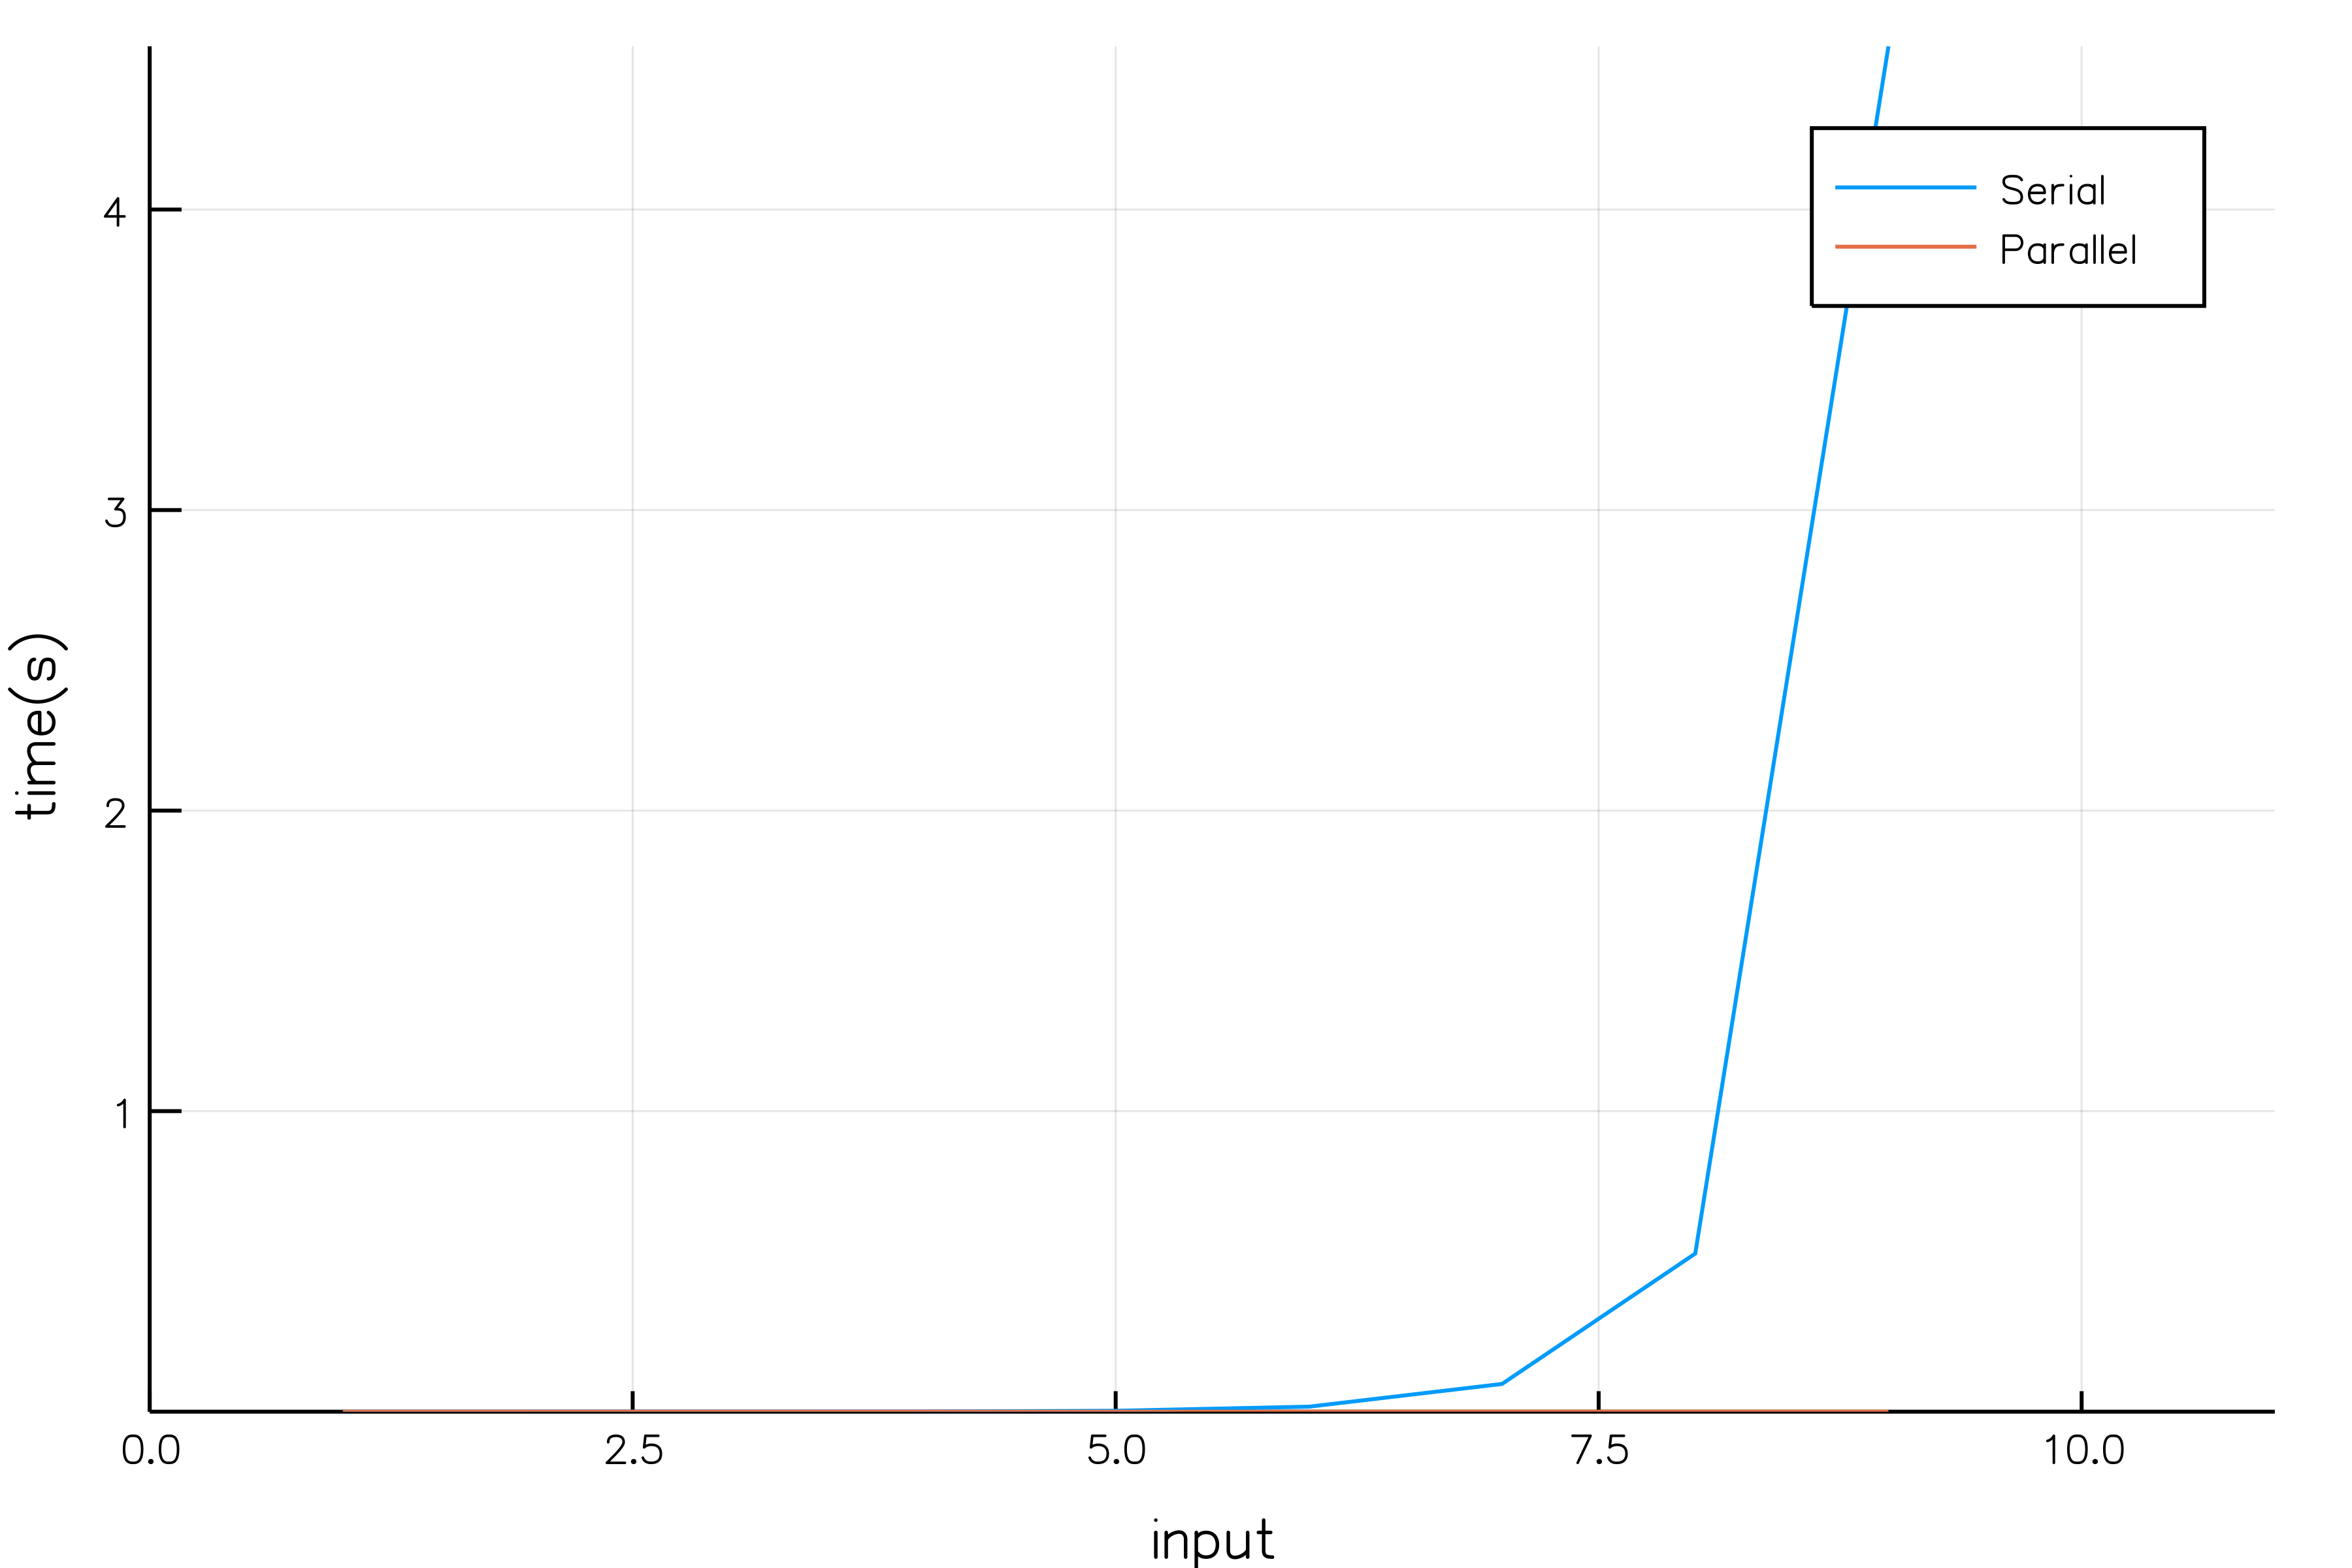
\includegraphics[width=11cm,scale=0.3]{boxC.png}
\end{figure}
\newpage
\subsection{traversal}
\subsubsection{Conversion}
\textbf{\emph{Python}}
 \lstset{language=Python}
\begin{lstlisting}
def traversal(CTM, stack, obj, scene=[]):
   for i in range(len(obj)):
      if isinstance(obj[i],Model): 
scene += [larApply(CTM)(obj[i])]
elif(isinstance(obj[i],tuple) or isinstance(obj[i],list)) and
(len(obj[i]==2 or len(obj[i])==3):
         scene += [larApply(CTM)(obj[i])]
      elif isinstance(obj[i],Mat): 
         CTM = scipy.dot(CTM, obj[i])
      elif isinstance(obj[i],Struct):
         stack.append(CTM) 
         traversal(CTM, stack, obj[i], scene)
         CTM = stack.pop()
   return scene
\end{lstlisting}
\textbf{\emph{Julia}}
\begin{lstlisting}[language=Julia, format=Julia]
function traversal(CTM,stack,obj,scene=[]){
for i in range(1,len(obj)){
 if isa(obj.body[i],Matrix){
CTM = CTM * obj.body[i]}
elseif (isa(obj.body[i],Tuple) || isa(obj.body[i],Array)) && {?
 (length(obj.body[i])==2 || length(obj.body[i])==3)
l=larApply(CTM)(obj.body[i])
push!(scene,l)}
elseif isa(obj.body[i],Struct){
push!(stack,CTM)	
traversal(CTM,stack,obj.body[i],scene)
CTM = pop!(stack)}
end}
end
return scene}
end
\end{lstlisting}
\subsubsection{Parallelization}
\begin{lstlisting}[language=Julia, format=Julia]
@everywhere function ptraversal(CTM,stack,obj,scene=[]){
@sync for i in range(1,len(obj)){
if isa(obj.body[i],Matrix){
CTM = CTM*obj.body[i]}
elseif (isa(obj.body[i],Tuple) || isa(obj.body[i],Array)) && {?(length(obj.body[i])==2 || length(obj.body[i])==3)
l=plarApply(CTM)(obj.body[i])
push!(scene,l)}}
elseif isa(obj.body[i],pStruct){
push!(stack,CTM)	
ptraversal(CTM,stack,obj.body[i],scene)
CTM = pop!(stack)}
end}
end
return scene}
end
\end{lstlisting}
\subsubsection{Unit-Test}
These tests can be runned after the definition of the Struct type on the section \ref{Struct}
\begin{lstlisting}[language=Julia]
@testset "traversal" begin
   square=([[0, 0], [0, 1], [1, 0], [1, 1]], [[0, 1, 2, 3]])
   @everywhere structure=Struct([square])
   @everywhere dim=checkStruct(structure.body)
   @test length(traversal(eye(dim+1),[],structure,[]))==length(structure.body)
   @test typeof(traversal(eye(dim+1),[],structure,[]))==Array{Any,1}
end



 square=([[0, 0], [0, 1], [1, 0], [1, 1]], [[0, 1, 2, 3]])
 structure=pStruct([square])
 dim=pcheckStruct(structure.body)
@testset "ptraversal" begin
  @test length(ptraversal(eye(dim+1),[],structure,[]))==length(structure.body)
  @test typeof(ptraversal(eye(dim+1),[],structure,[]))==Array{Any,1}
end
\end{lstlisting}
\subsubsection{Results}
\textbf{Tesla}
\begin{lstlisting}[language=Julia]
input=[1,10,50,10^2,5*10^2,10^3,5*10^3,10^4,5*10^4,10^5,5*10^5,10^6]
	    
function timeTraversal(model,input)
   t=Array{Float64}(length(input))
   pt=Array{Float64}(length(input))
   for i in range(1,length(input))
      structo=addn2D(input[i],model)
      pstructo=pStruct(structo.body)
      dim=checkStruct(structo.body)
      traversal(eye(dim+1),[],structo,[])
      ptraversal(eye(dim+1),[],pstructo,[])
      pt[i]=@elapsed ptraversal(eye(dim+1),[],pstructo,[])
      t[i]=@elapsed traversal(eye(dim+1),[],structo,[])
   end
   return t,pt
end

y,yp=timeTraversal(square,input)
p=plot(y,xaxis=''input'',yaxis=''time'',xlims=(0,length(input)+1),
       ylims=(0,maximum(y)+0.5), label=[''Serial''],lw=2)
\end{lstlisting}
\begin{figure}[ht!]
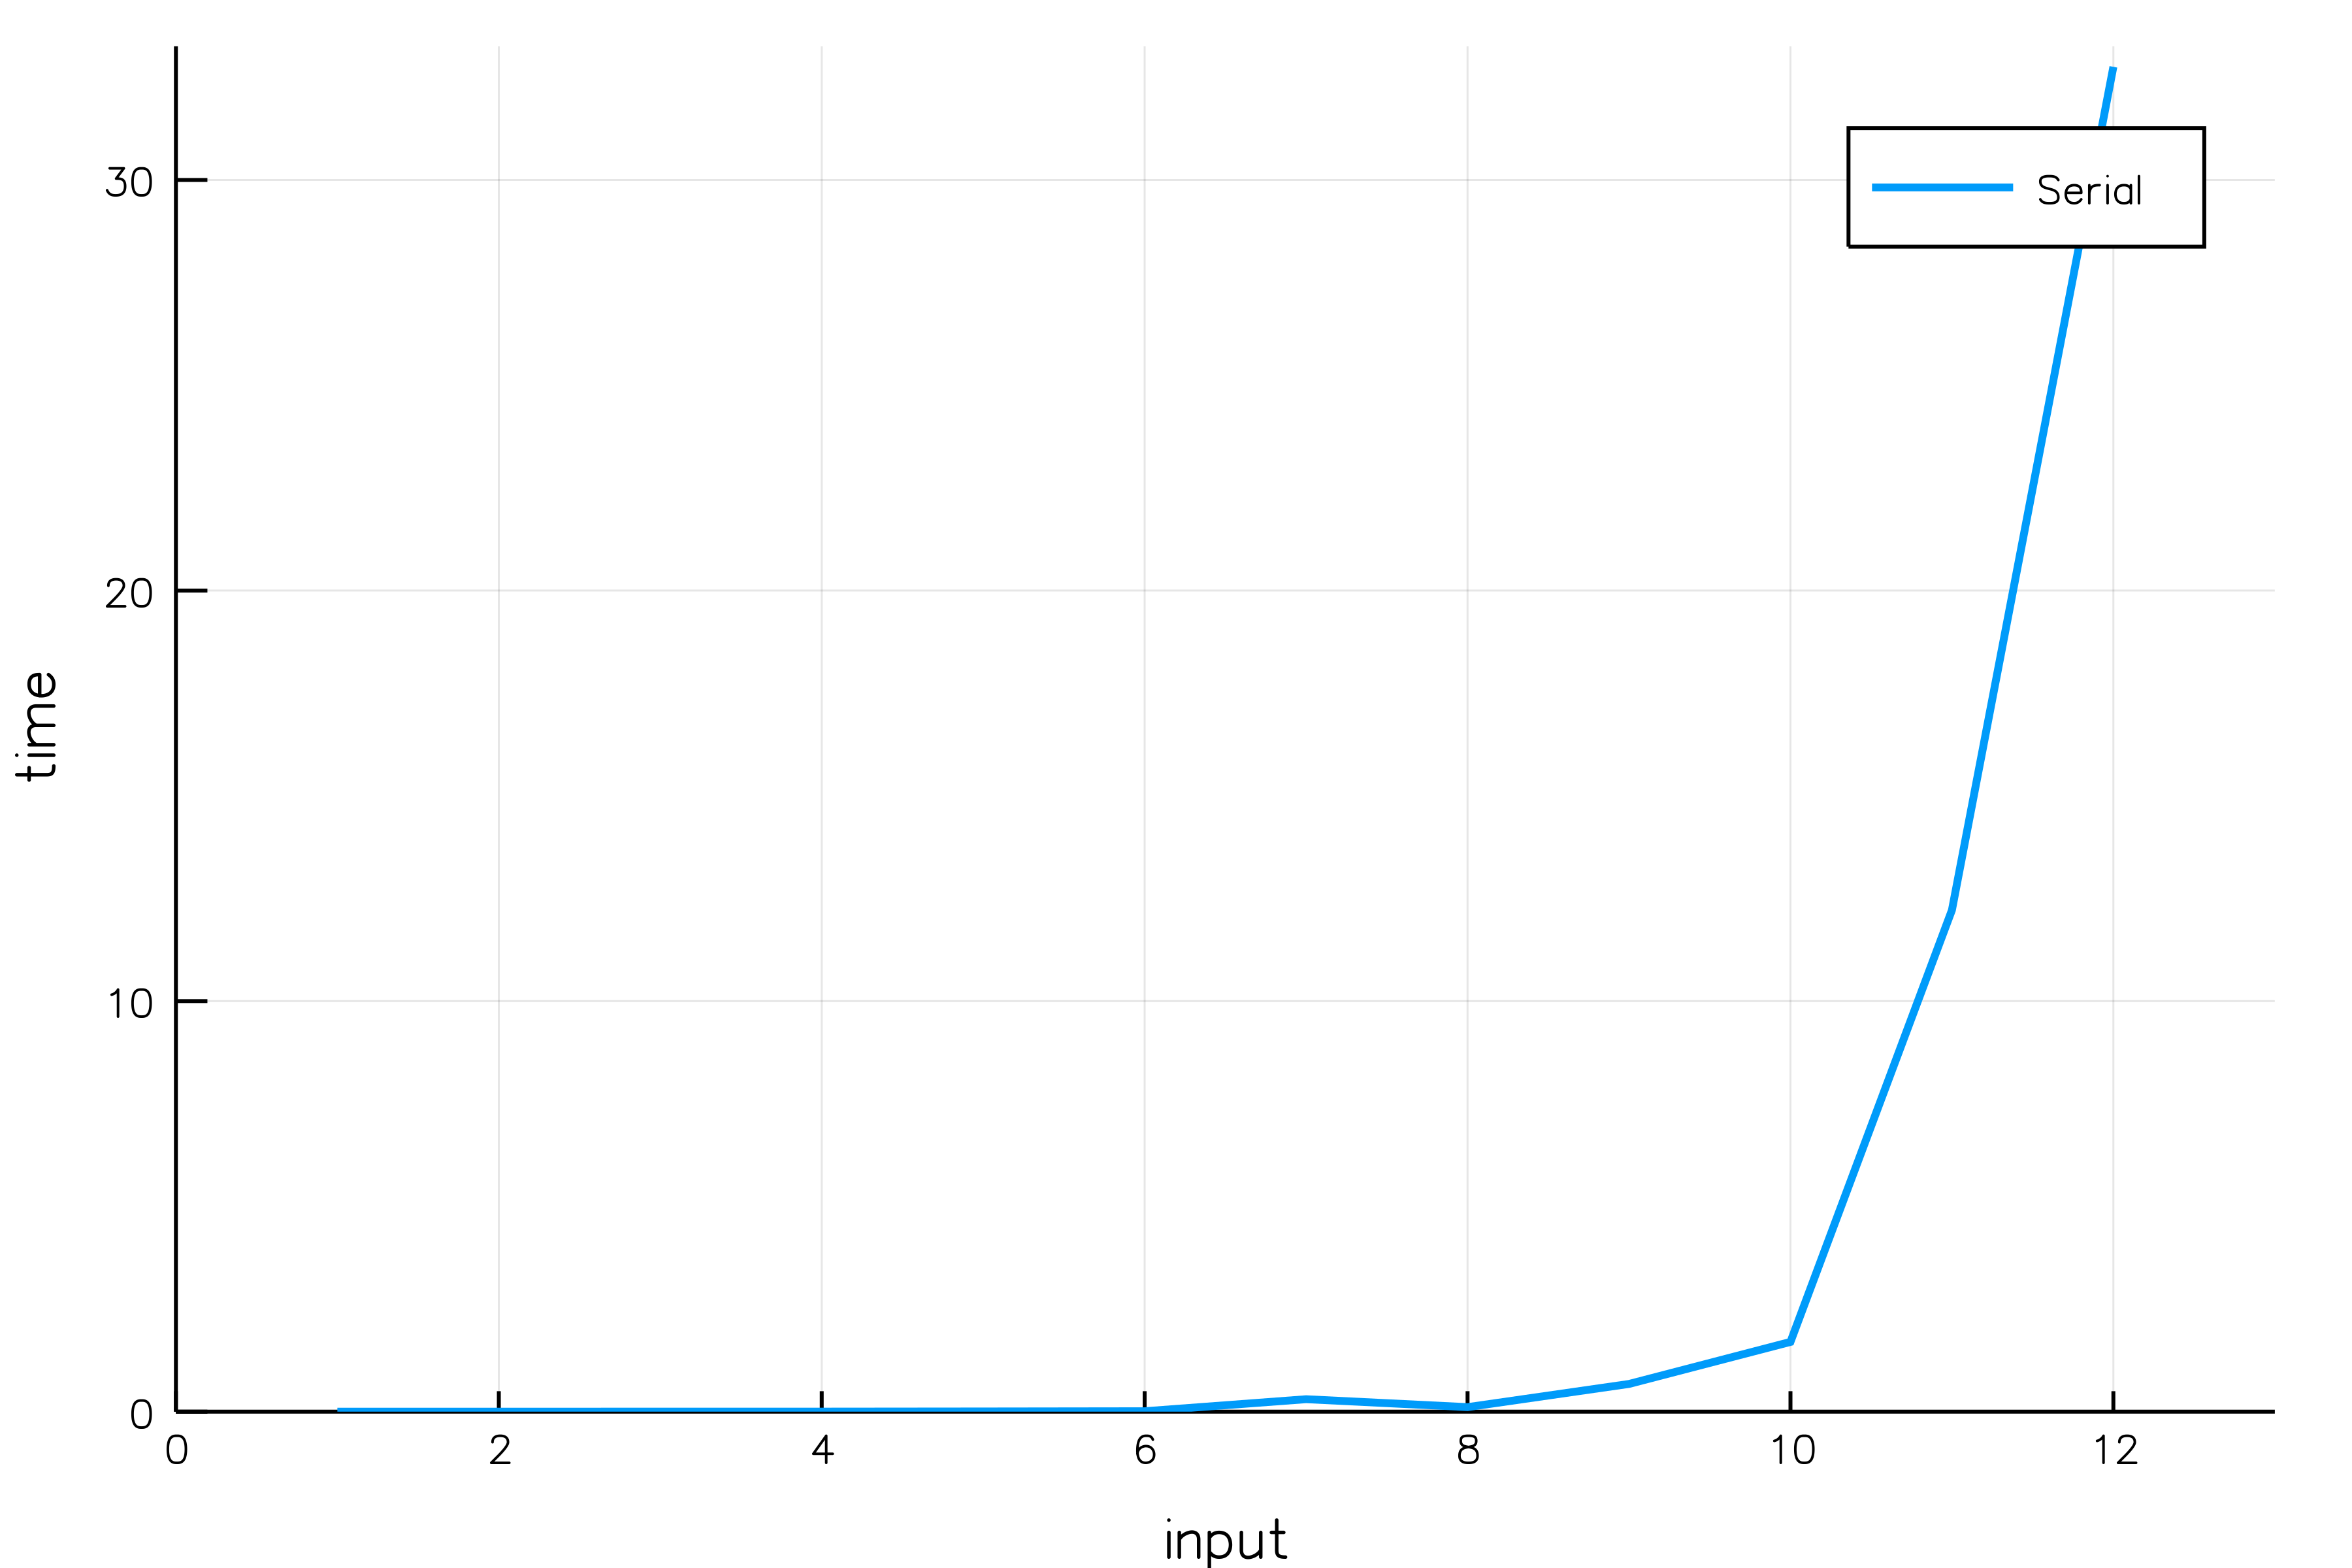
\includegraphics[width=13cm,scale=0.3]{traversal.png}
\end{figure}
\newpage
\begin{verbatim}
pp=plot(yp,xaxis=''input'',yaxis=''time'',xlims=(0,length(input)+1),
       ylims=(0,maximum(y)+0.5),label=[''Parallel''],lw=2)
\end{verbatim}
\begin{figure}[ht!]
\centering
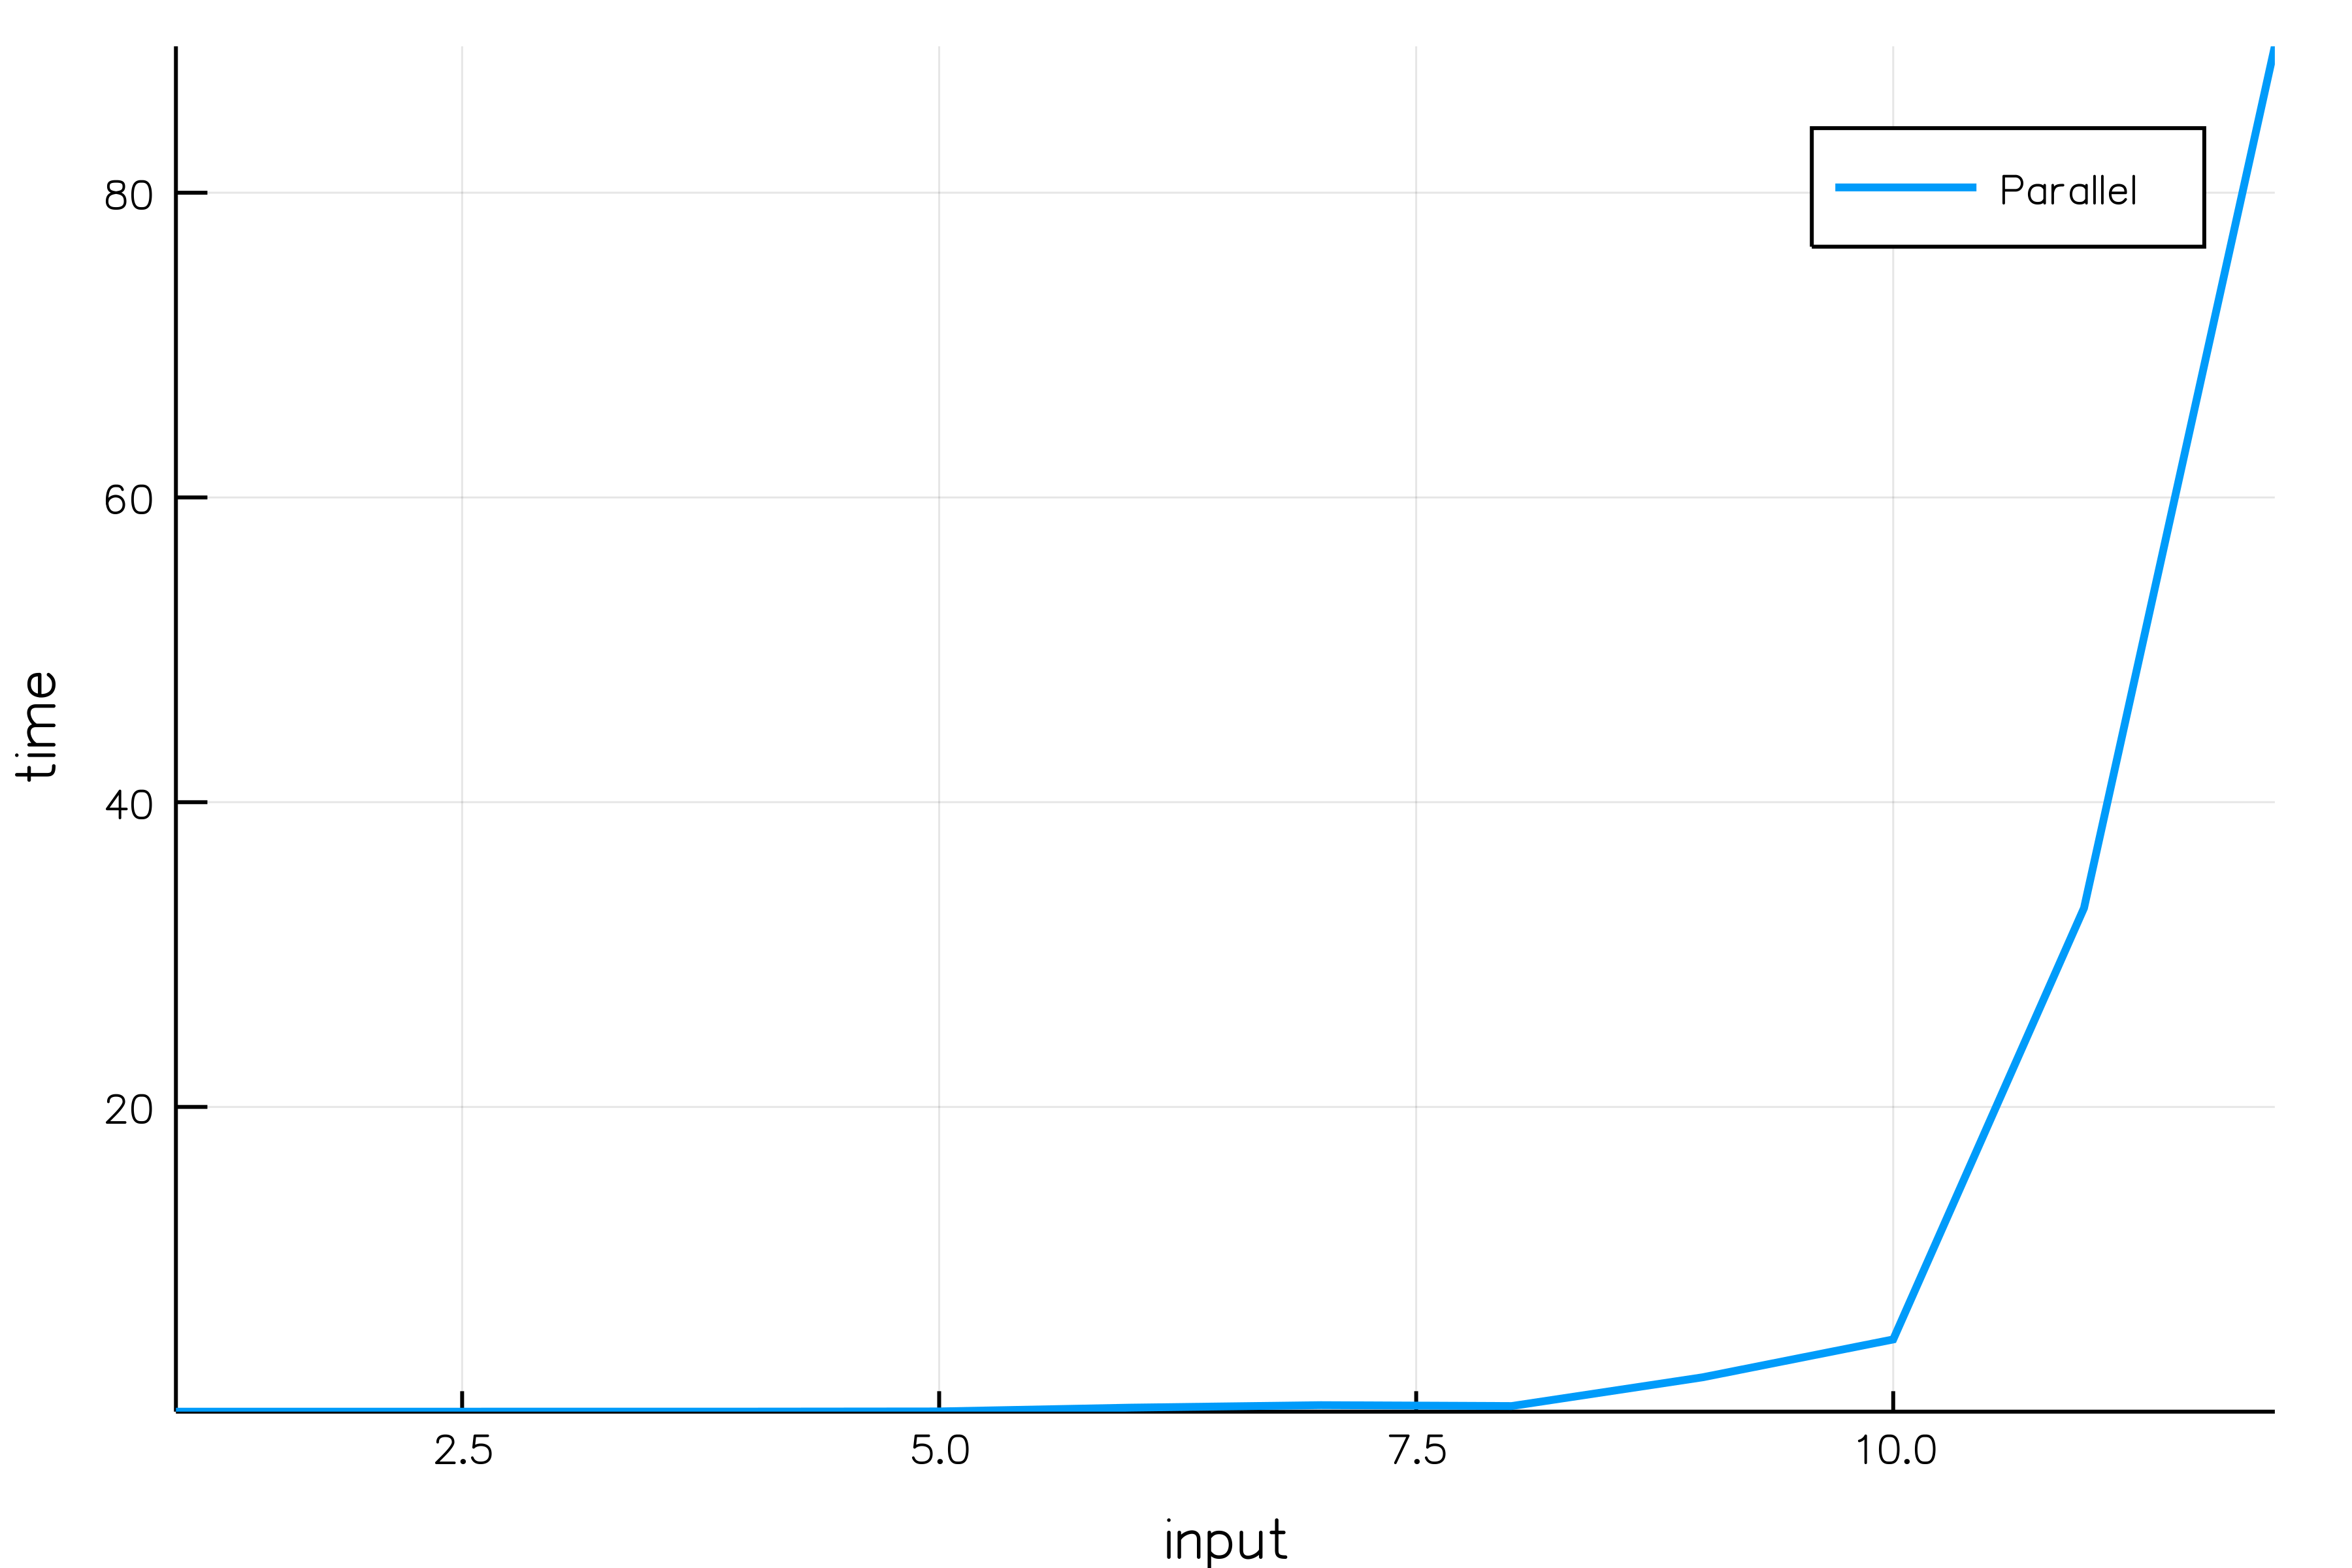
\includegraphics[width=11cm,scale=0.3]{ptraversal.png}
\end{figure}
\begin{verbatim}
yc=[y,yp]
pc=plot(yc,label=["Serial" "Parallel"])
\end{verbatim}
\begin{figure}[ht!]
\centering
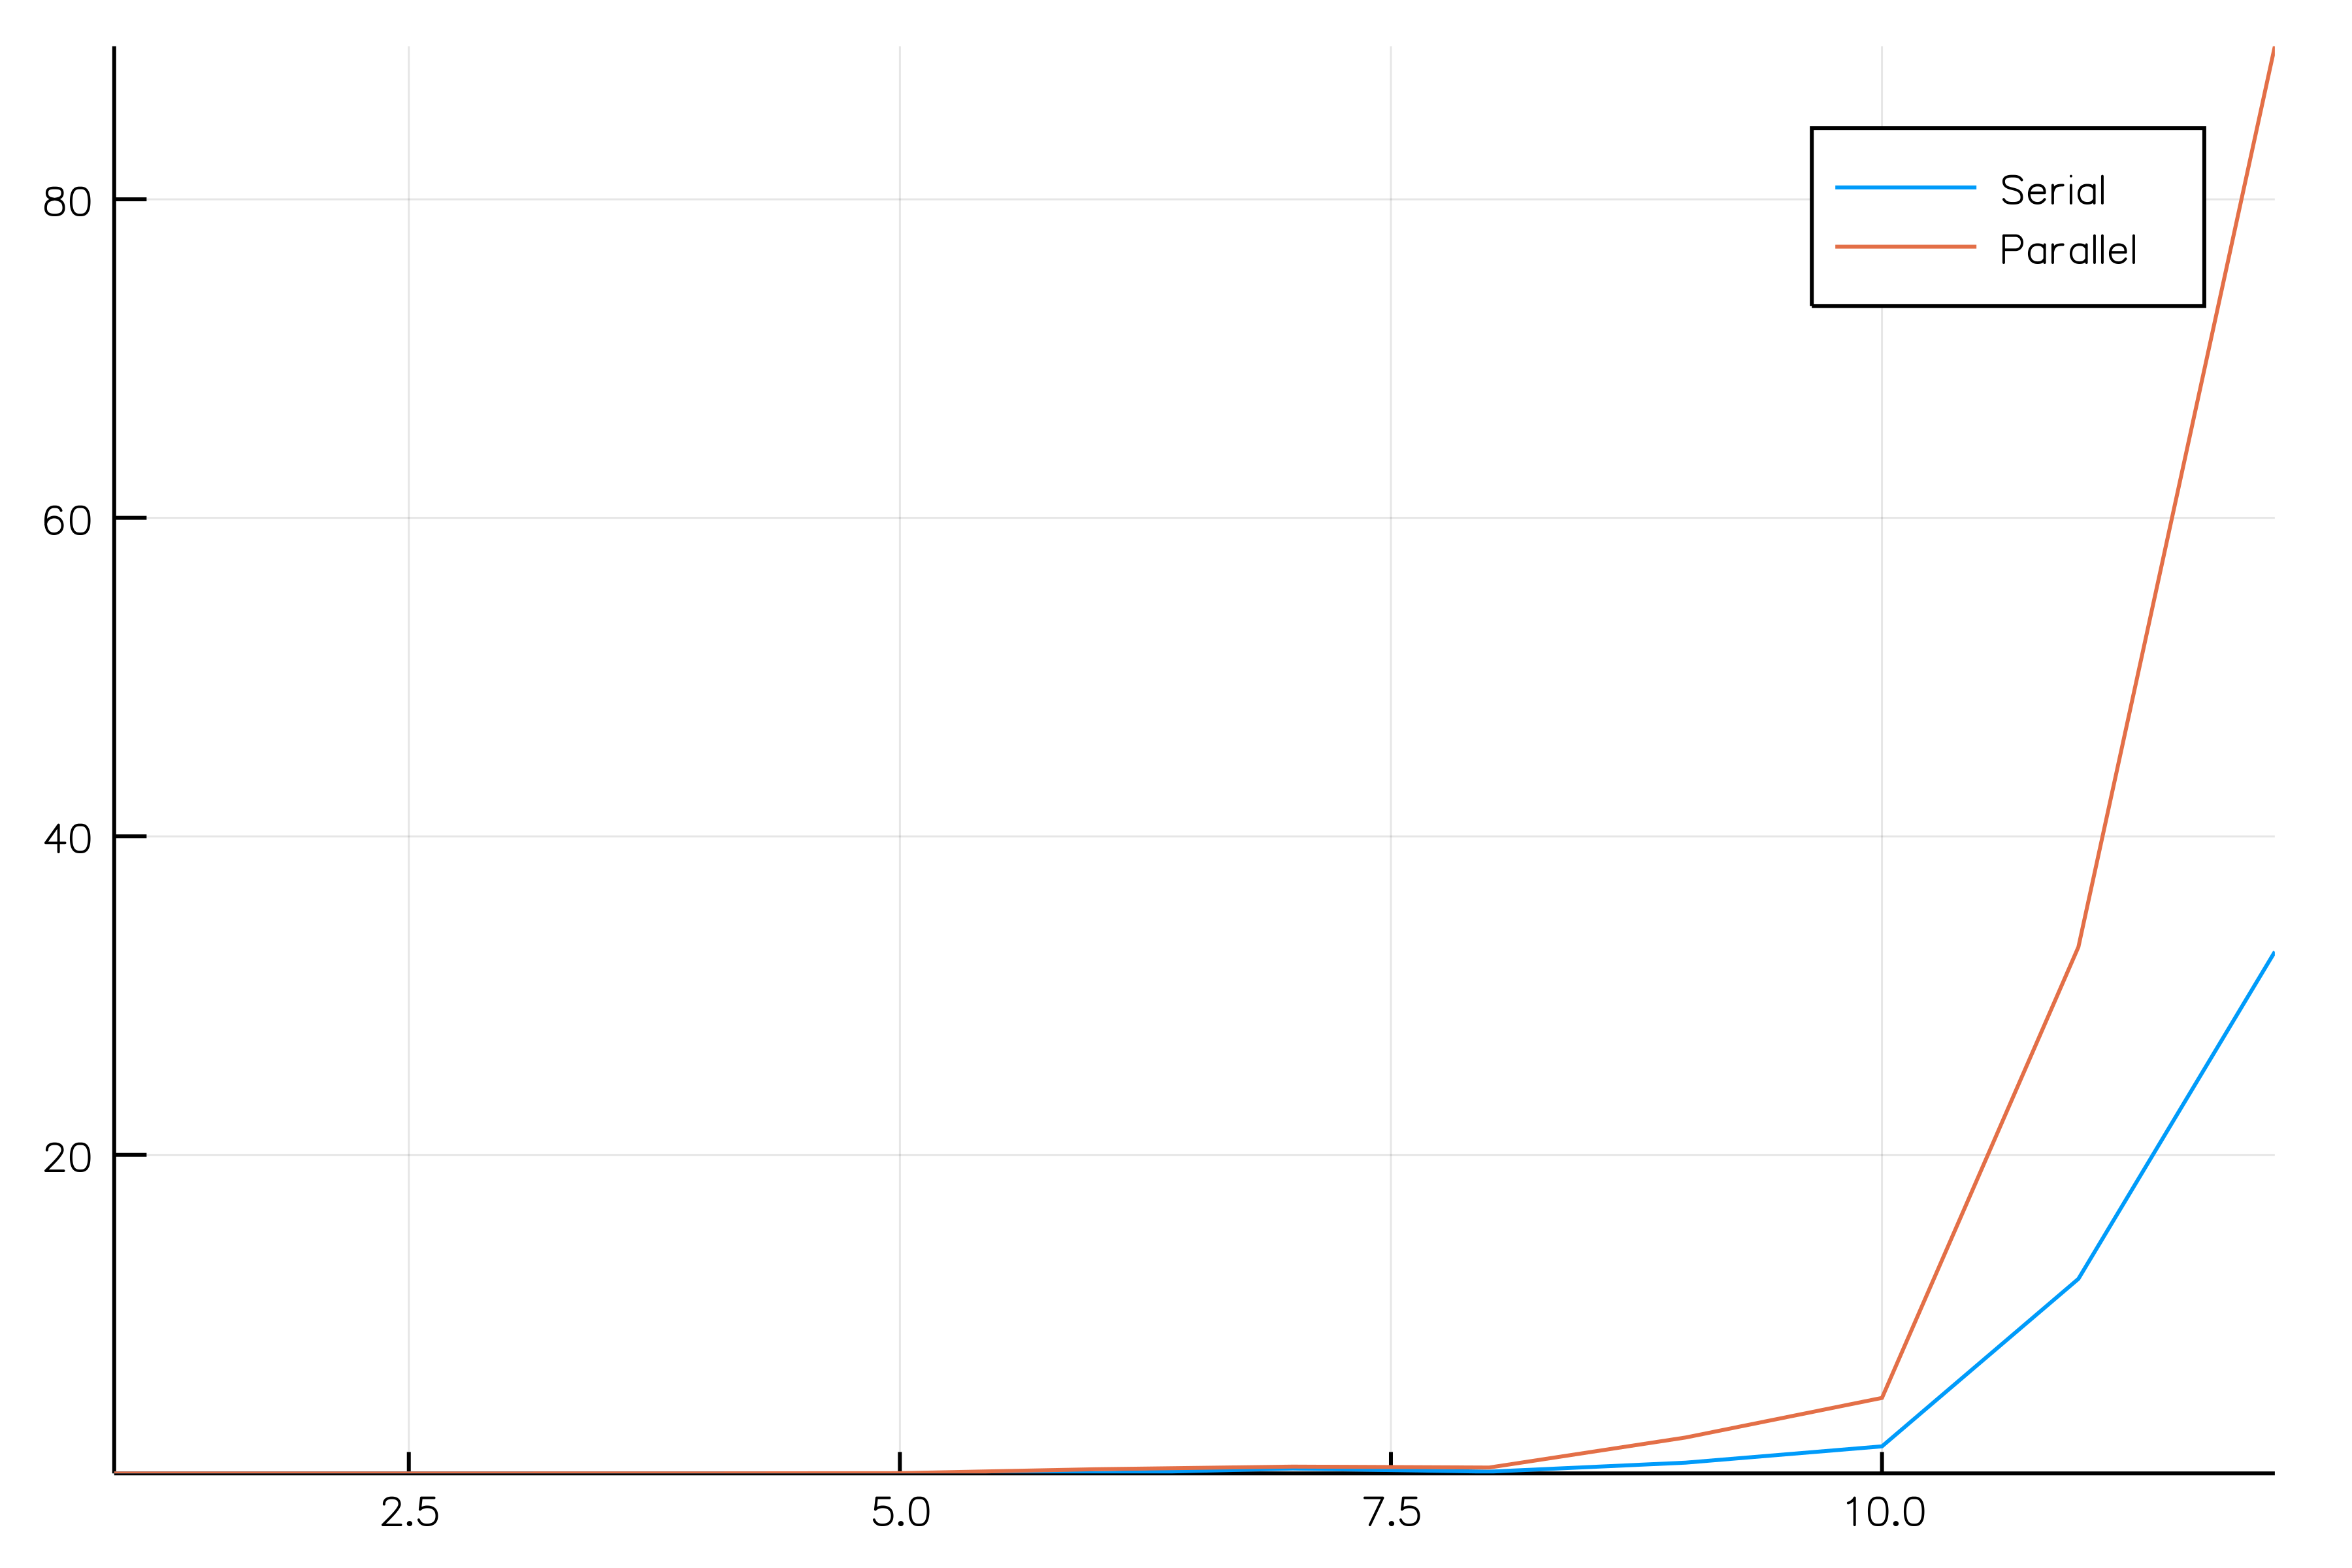
\includegraphics[width=11cm,scale=0.5]{comptraversal.png}
\end{figure}
\newpage
\textbf{PC}
\begin{lstlisting}[language=Julia,format=Julia]
times=[ ]
ptimes=[ ]
input=[ ]
dim=[ ]
for i in range(1,length(l)-1){
	push!(input,Struct([repeat([l[i]],outer=i)...]))}
end
for i in range(1,length(l)-1){
	append!(dim,checkStruct(input[i].body))}
end
for i in range(1,length(input)){
	args=(eye(dim[i]+1),[],input[i],[])
	append!(times,Time(traversal,(args...)))}
end
for i in range(1,length(input)){
	args=(eye(dim[i]+1),[],input[i],[])
	append!(ptimes,Time(ptraversal,(args...)))}
end

plot(times,xlabel="input",xlims=(0,length(times)+2),{?ylabel="time(s)",label=["Serial"])
\end{lstlisting}
\begin{figure}[ht!]
\centering
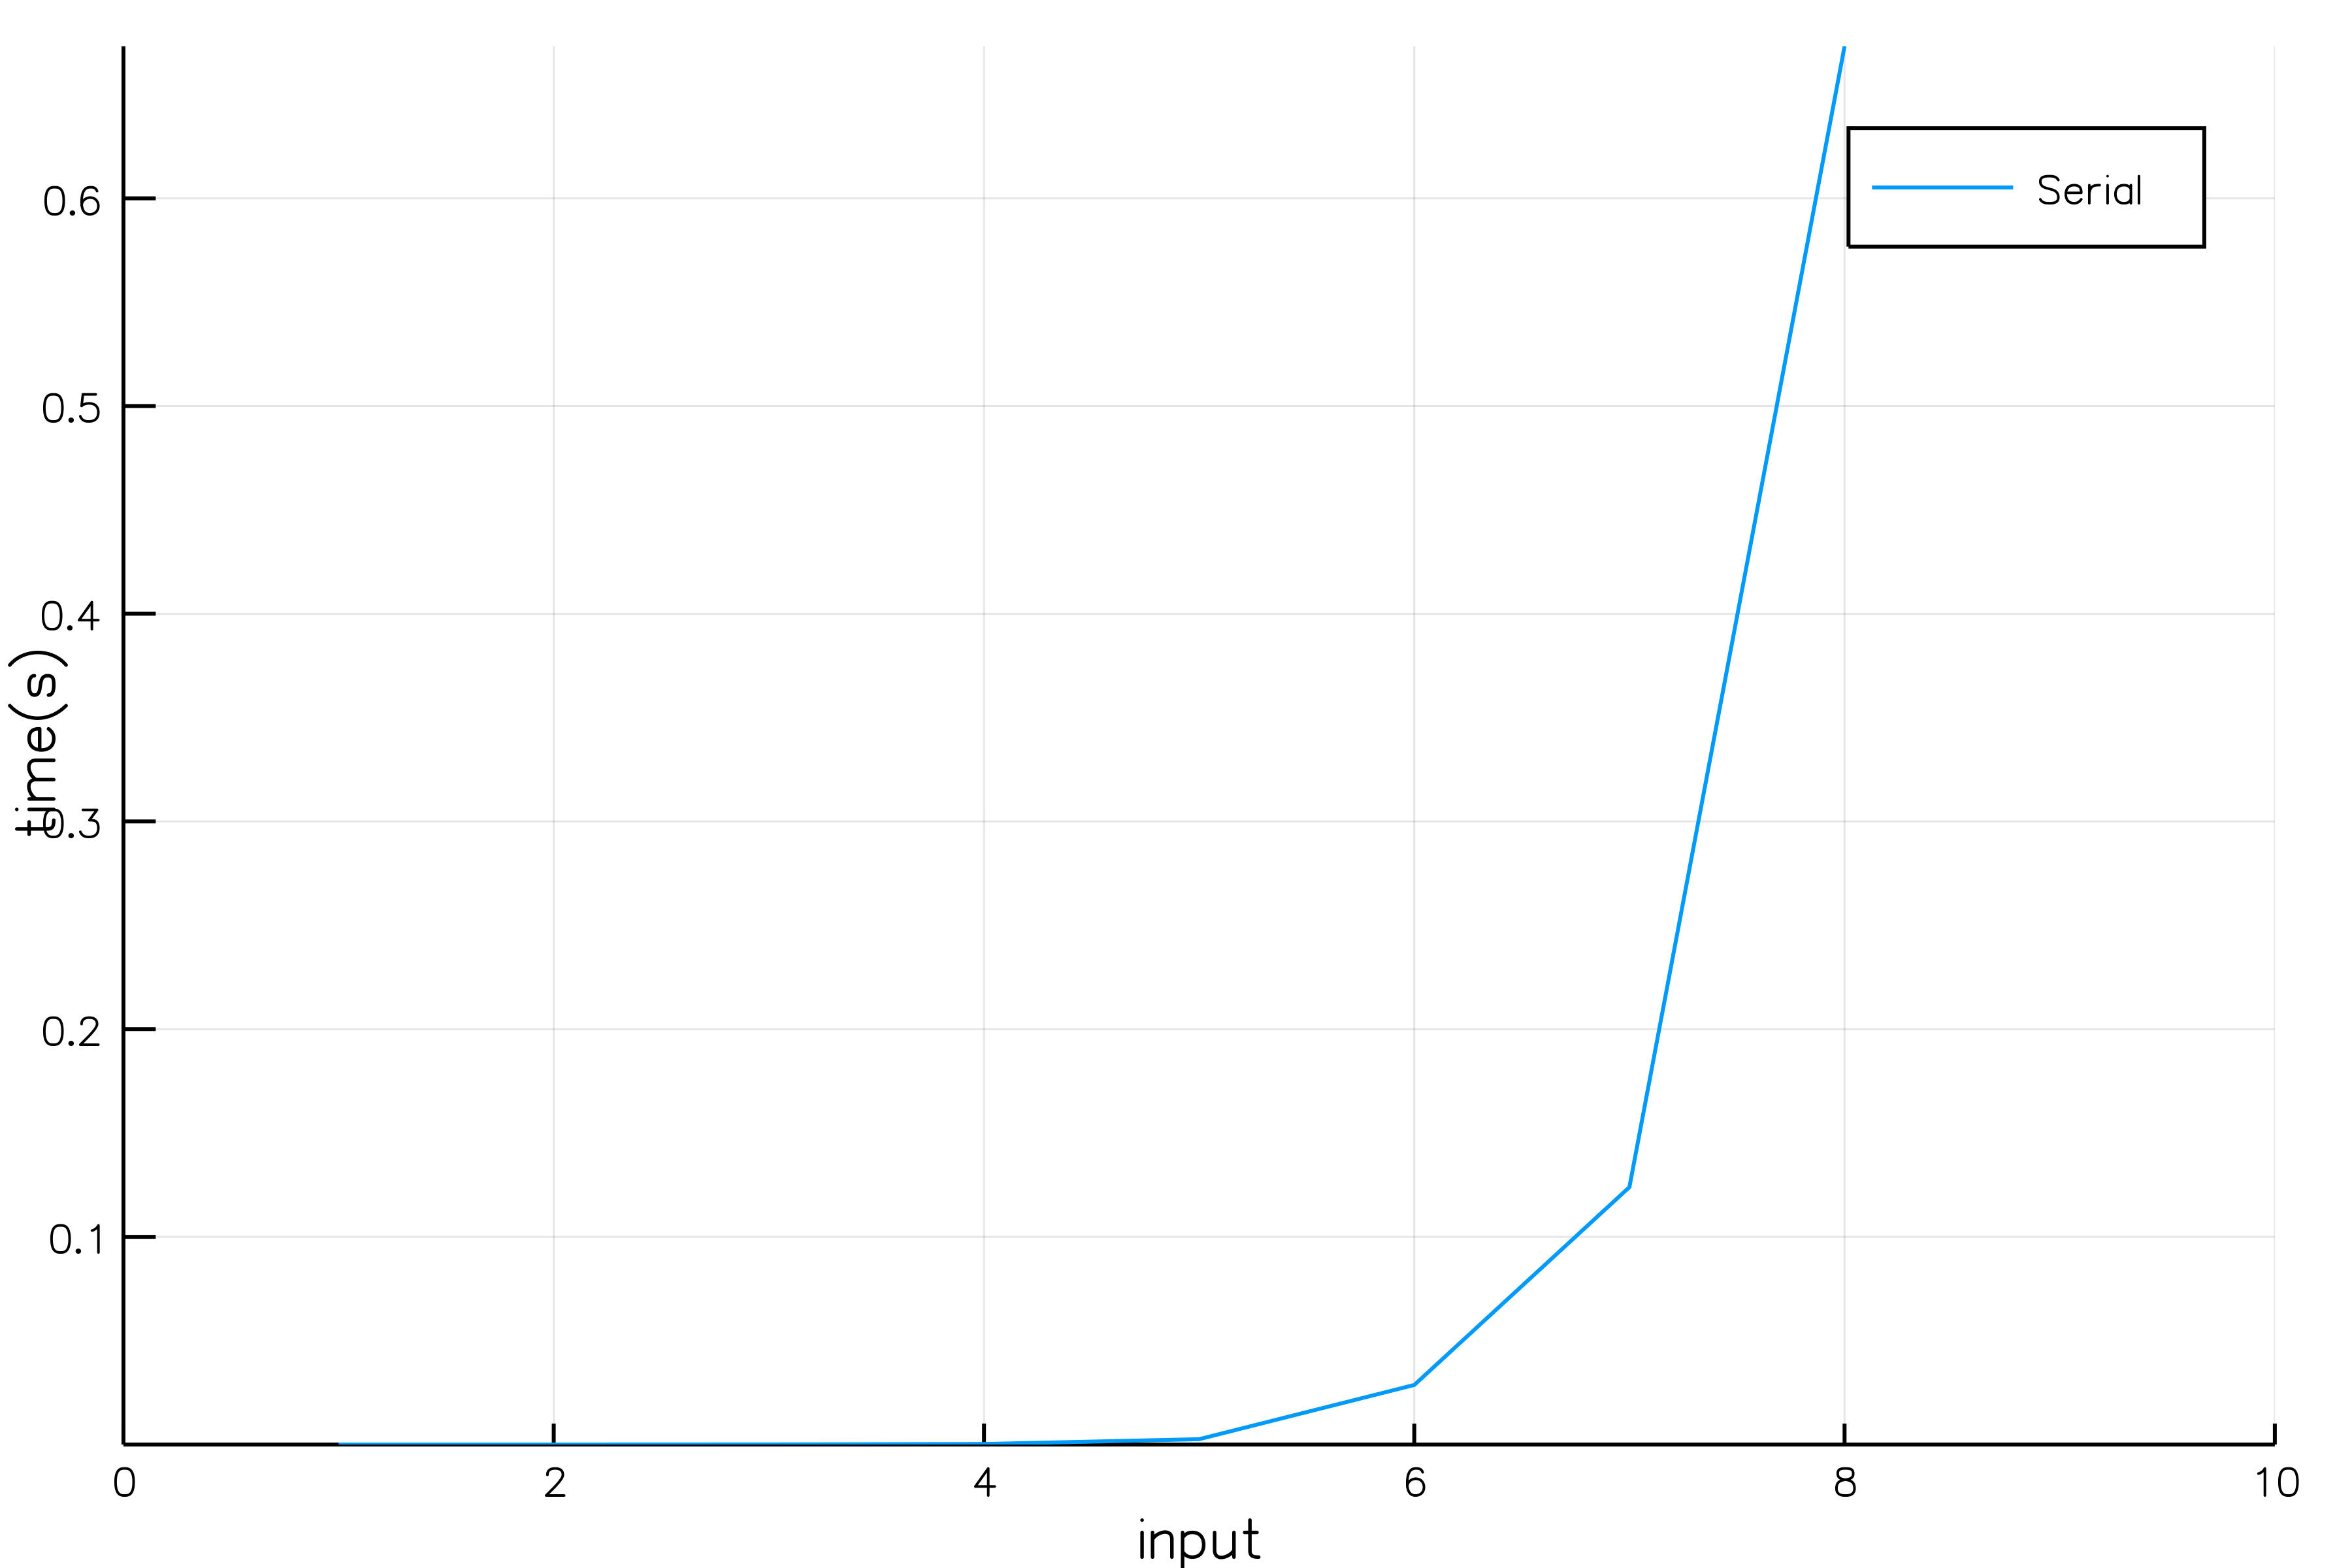
\includegraphics[width=11cm,scale=0.5]{traversalSerial.png}
\end{figure}
\begin{lstlisting}[language=Julia]
plot(ptimes,xlabel="input",xlims=(0,length(times)+2),
   ylabel="time(s)",label=["Parallel"]
\end{lstlisting}
\begin{figure}[ht!]
\centering
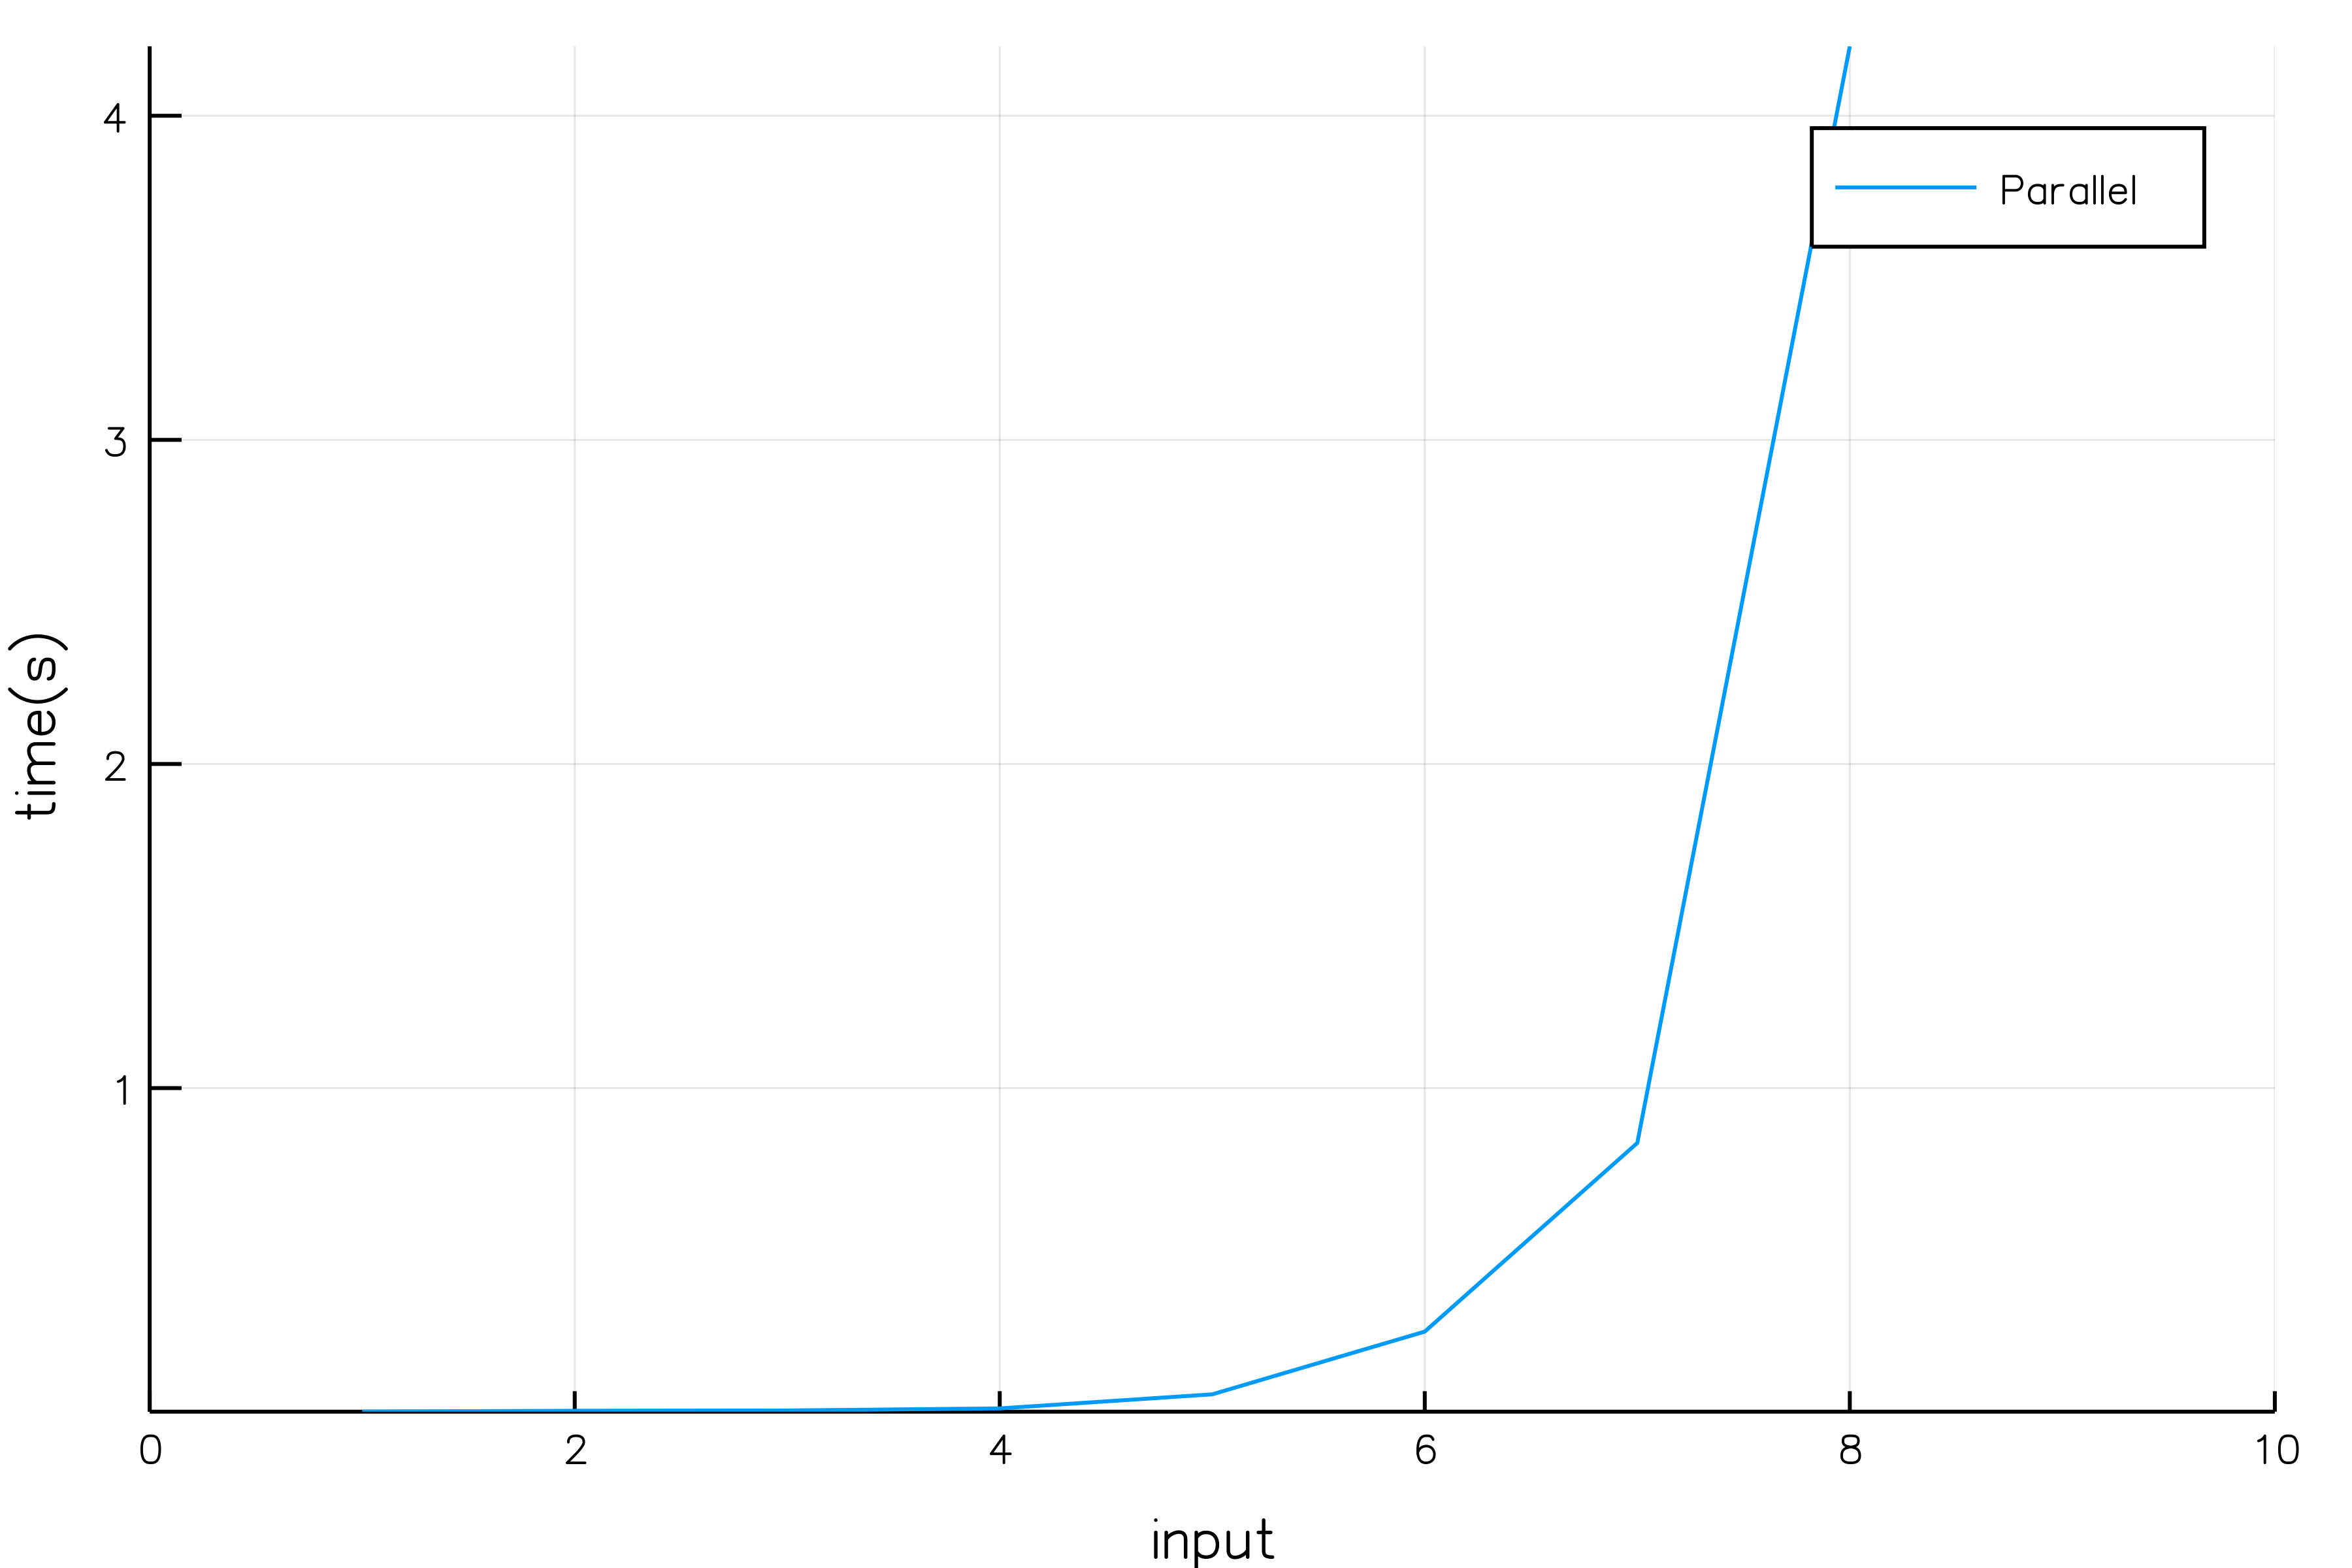
\includegraphics[width=11cm,scale=0.5]{traversalParallel.png}
\end{figure}
\begin{lstlisting}[language=Julia]
plot([times,ptimes],xlabel="input",xlims=(0,length(ptimes)+2),
  ylabel="time(s)",label=["Serial","Parallel"])
\end{lstlisting}
\begin{figure}[ht!]
\centering
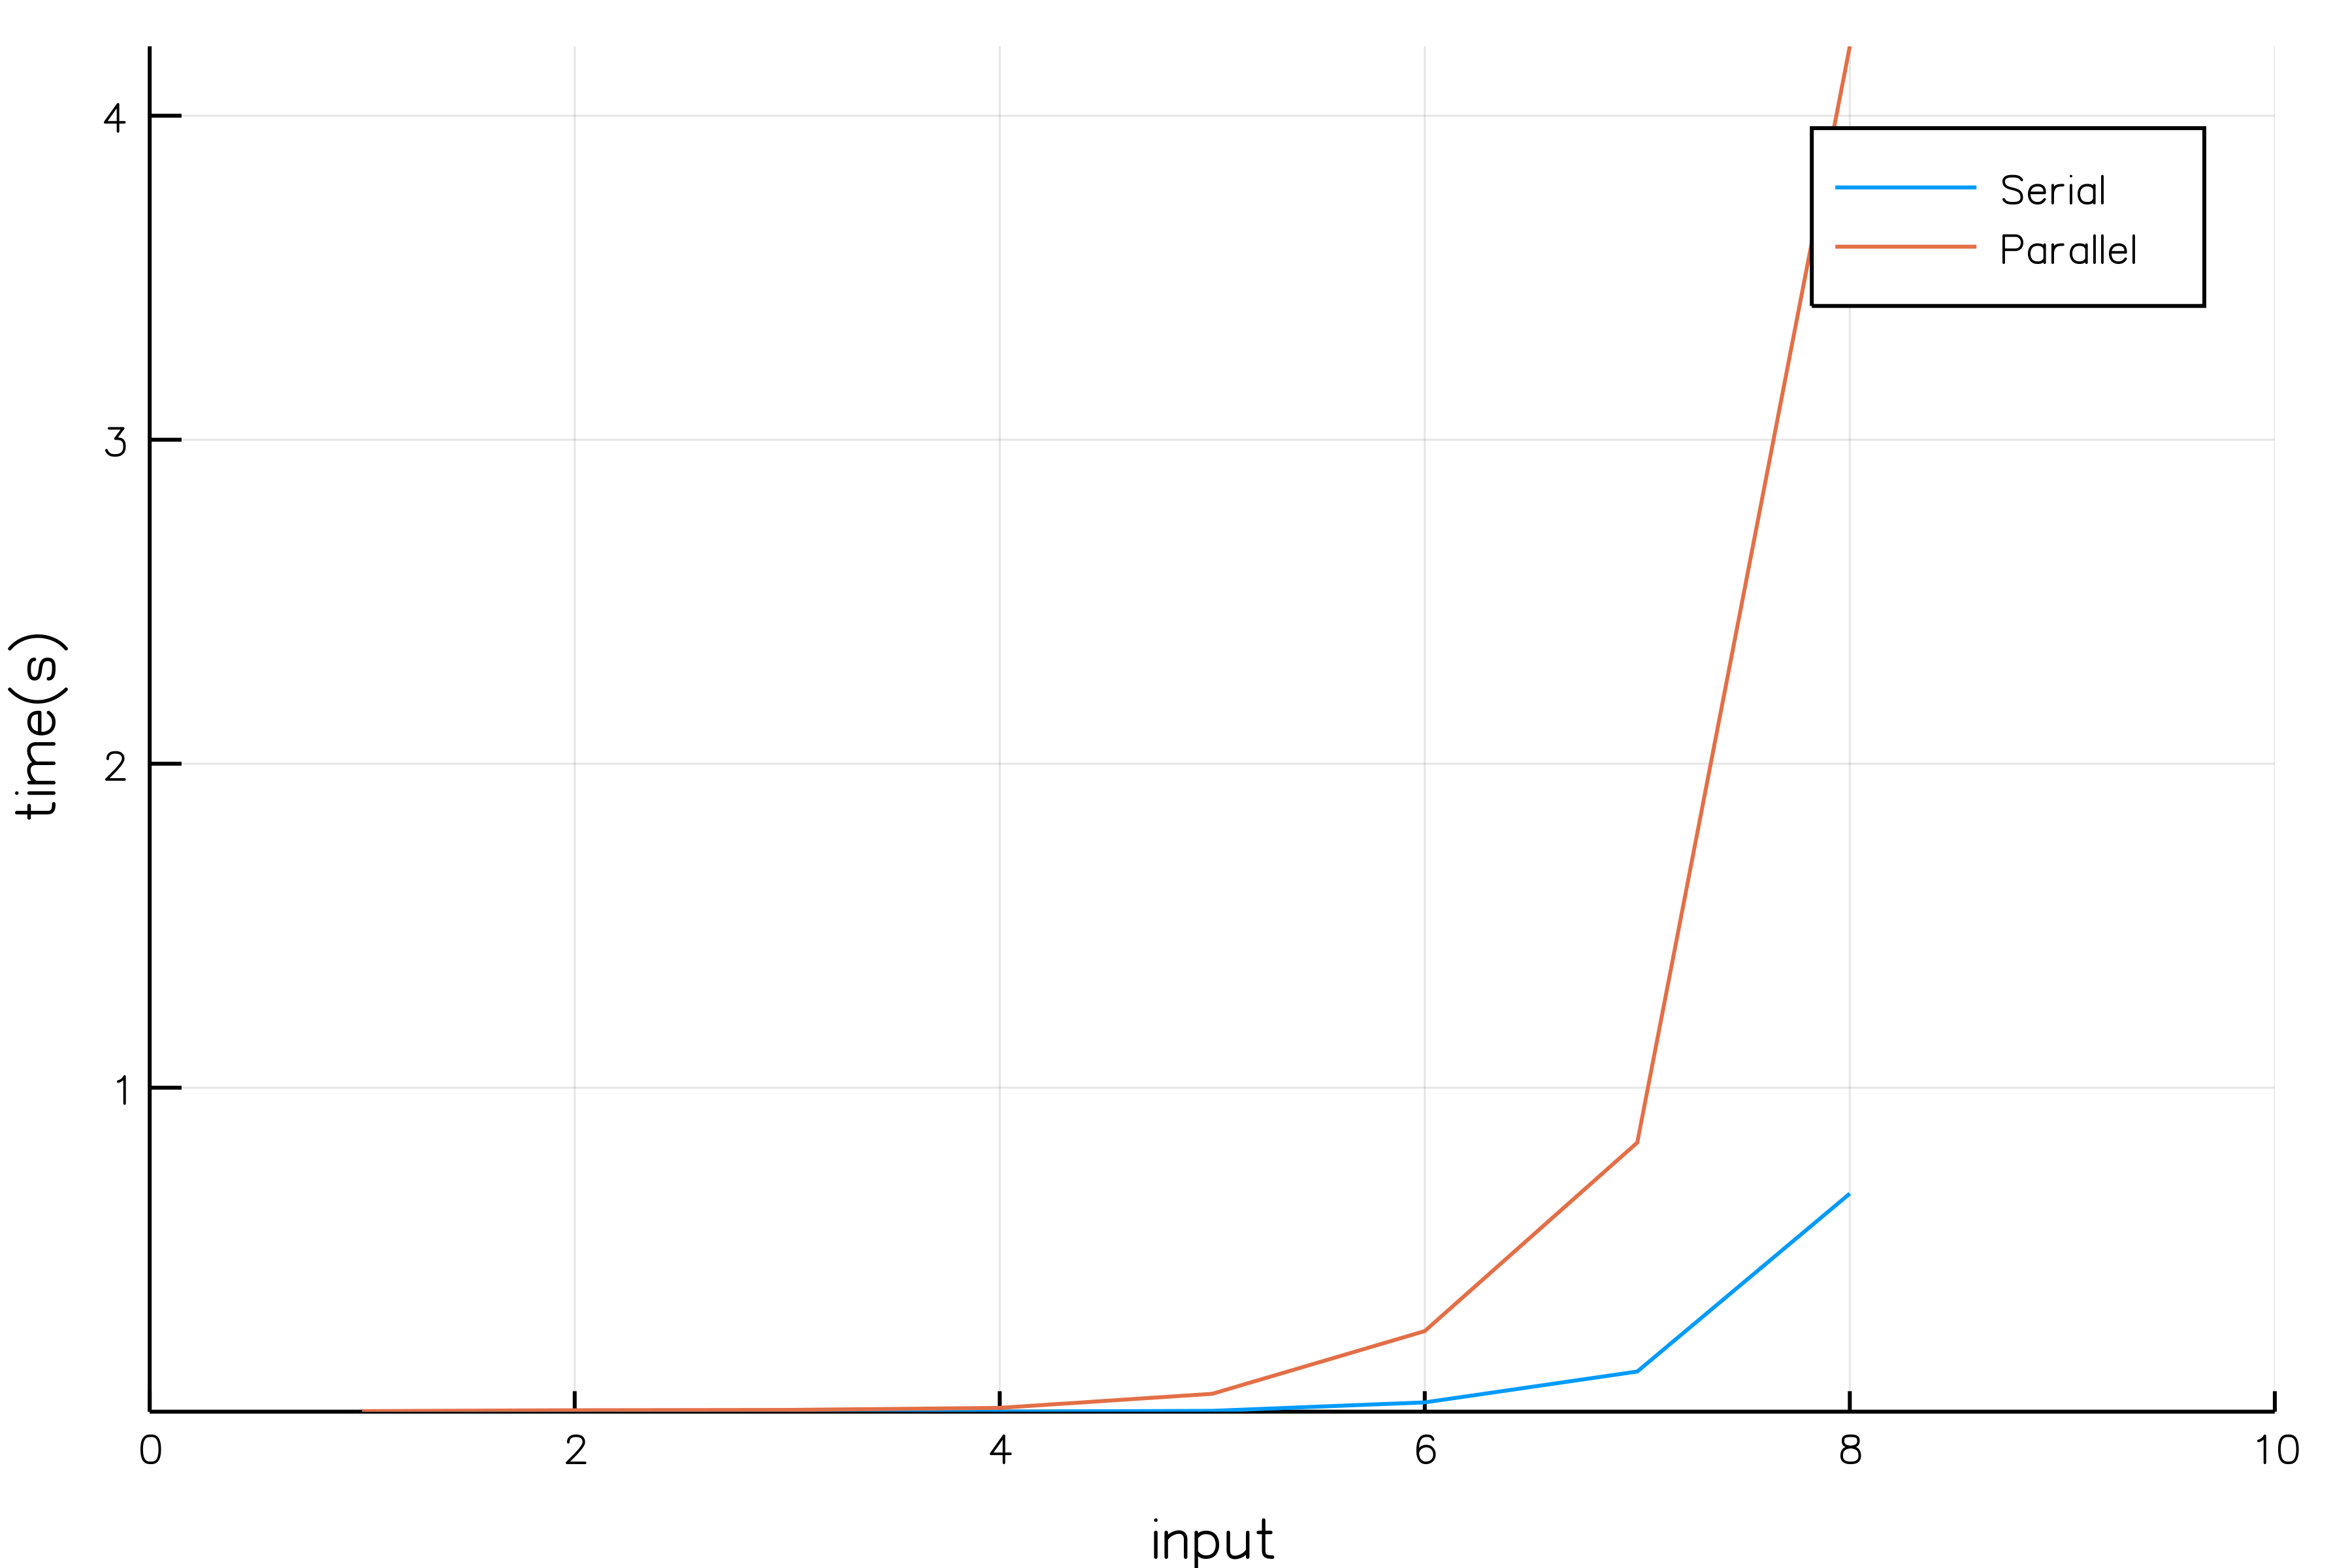
\includegraphics[width=11cm,scale=0.5]{traversalC.png}
\end{figure}
\newpage
\subsection{Struct}\label{Struct}
\subsubsection{Conversion}
\textbf{Python}
\begin{lstlisting}[language=Python,format=Julia]
def evalStruct(struct):{
    dim = checkStruct(struct.body)
    CTM, stack = scipy.identity(dim+1), [ ]
    scene = traversal(CTM, stack, struct, [ ]) 
    return scene}

class Struct:{
       def __init__(self,data=None,name=None,category=None):{
        if data==None or data==[ ]:{
            self.body = [ ]}
        else:{
            #self.body = [item for item in data if item != None]
            self.body = [item for item in data]
            self.box = box(self) 
            self.dim = len(self.box[0])}
        if name != None:{ 
            self.name = str(name)}
        else:{
            self.name = str(id(self))}
        if category != None: {
            self.category = str(category)}
        else:{
            self.category = "feature"}
    def __name__(self):{
        return self.name}
    def __category__(self):{
        return self.category}
    def __iter__(self):{
        return iter(self.body)}
    def __len__(self):{
        return len(list(self.body))}
    def __getitem__(self,i):{
        return list(self.body)[i]}
    def __setitem__(self,i,value):{
        self.body[i] = value}
    def __print__(self): {
        return "<Struct name: %s>" % self.__name__()}
    def __repr__(self):{
        return "<Struct name: %s>" % self.__name__()}
     def set_name(self,name):{
        self.name = str(name)}
    def clone(self,i=0):{
        from copy import deepcopy
        newObj = deepcopy(self)
        if i != 0: newObj.name = self.name + "_" + str(i)
        return newObj}
    def set_category(self,category):{
        self.category = str(category)
\end{lstlisting}
\textbf{Julia}
\begin{lstlisting}[language=Julia,format=Julia]
function evalStruct(self){
	dim = checkStruct(self.body)
   	CTM, stack = eye(dim+1), []
   	scene = traversal(CTM, stack, self, []) 
return scene}
end

\end{lstlisting}
\begin{lstlisting}[language=Julia]
type Struct
	body::Array
	box
	name::AbstractString
	dim
	category::AbstractString
	
	function Struct()
		self=new([],Nullable{Any},"new",Nullable{Any},"feature")
		self.name=string(object_id(self))
		return self
	end
	function Struct(data::Array)
		self=Struct()
		self.body=data
		self.box=box(self)
		self.dim=length(self.box[1])
		return self
	end	
	function Struct(data::Array,name)
		self=Struct()
		self.body=[item for item in data]
		self.box=box(self)
		self.dim=length(self.box[1])
		self.name=string(name)
		return self
	end
	function Struct(data::Array,name,category)
		self=Struct()
		self.body=[item for item in data]
		self.box=box(self)
		self.dim=length(self.box[1])
		self.name=string(name)
		self.category=string(category)
		return self
	end
end
	function name(self::Struct)
		return self.name
	end
	function category(self::Struct)
		return self.category
	end
	function len(self::Struct)
		return length(self.body)
	end
	function getitem(self::Struct,i::Int)
		return self.body[i]
	end
	function setitem(self::Struct,i,value)
		self.body[i]=value
	end
	function pprint(self::Struct)
		return "<Struct name: $(self.__name__())"
	end
	function set_name(self::Struct,name)
		self.name=string(name)
	end
	function clone(self::Struct,i=0)
		newObj=deepcopy(self)
		if i!=0
			newObj.name="$(self.__name__())_$(string(i))"
		end
		return newObj
	end
	function set_category(self::Struct,category)
		self.category=string(category)
	end
\end{lstlisting}
\subsubsection{Parallelization}
\begin{lstlisting}[language=Julia,format=Julia]
function pevalStruct(self){
	dim = pcheckStruct(self.body)
   	CTM, stack = eye(dim+1), []
   	scene = ptraversal(CTM, stack, self, []) 
return scene}
end

\end{lstlisting}
\begin{lstlisting}[language=Julia]
@everywhere type pStruct
	body::Array
	box
	name::AbstractString
	dim
	category::AbstractString
	
	function pStruct()
		self=new([],Nullable{Any},"new",Nullable{Any},"feature")
		self.name=string(object_id(self))
		return self

	end
	function pStruct(data::Array)
		self=pStruct()
		self.body=data
		self.box=pbox(self)
		self.dim=length(self.box[1])
		return self
	end
	function pStruct(data::Array,name)
		self=pStruct()
		self.body=[item for item in data]
		self.box=pbox(self)
		self.dim=length(self.box[1])
		self.name=string(name)
		return self
	end
	function pStruct(data::Array,name,category)
		self=pStruct()
		self.body=[item for item in data]
		self.box=pbox(self)
		self.dim=length(self.box[1])
		self.name=string(name)
		self.category=string(category)
		return self
	end
end
	function name(self::pStruct)
		return self.name
	end
	function category(self::pStruct)
		return self.category
	end
	function len(self::pStruct)
		return length(self.body)
	end
	function getitem(self::pStruct,i::Int)
		return self.body[i]
	end
	function setitem(self::pStruct,i,value)
		self.body[i]=value
	end
	function pprint(self::pStruct)
		return "<Struct name: $(self.__name__())"
	end
	function set_name(self::pStruct,name)
		self.name=string(name)
	end
	function clone(self::pStruct,i=0)
		newObj=deepcopy(self)
		if i!=0
			newObj.name="$(self.__name__())_$(string(i))"
		end
		return newObj
	end
	function set_category(self::pStruct,category)
		self.category=string(category)
	end
\end{lstlisting}
\subsubsection{Unit-Test}
\begin{lstlisting}[language=Julia,format=Julia]
square=([[0,0],[0,1],[1,0],[1,1]],[[0,1,2,3]])

@testset "Struct Tests" begin{
	@test Struct([square]).body==[square]
	@test Struct([square]).dim==length(square[1][1])
	@test Struct([square]).box==[[0,0],[1,1]]}
end

square=([[0,0],[0,1],[1,0],[1,1]],[[0,1,2,3]])
@testset "pStruct Tests" begin{
@test pStruct([square]).body==[square]{
	@test pStruct([square]).dim==length(square[1][1])
	@test pStruct([square]).box==[[0,0],[1,1]]
	@test pStruct([square]).category=="feature"
	@test pStruct([square],"quadrato").name=="quadrato"}
end
\end{lstlisting}
\subsubsection{Results}
\begin{lstlisting}[language=Julia]
input=[1,10,50,10^2,5*10^2,10^3,5*10^3,10^4,5*10^4,10^5,5*10^5,10^6]
function timeStruct(model,input)
	t=Array{Float64}(length(input))
	pt=Array{Float64}(length(input))
	for i in range(1,length(input))
	    structo=addn2D(input[i],model)
	    Struct(structo.body)
	    pStruct(structo.body)
	    t[i]=@elapsed  Struct(structo.body)
	    pt[i]=@elapsed pStruct(structo.body)
	end
	return t,pt
end

y,yp=timeStruct(square,input)
p=plot(y,xaxis=''input'',yaxis=''time'',xlims=(0,length(input)+1),
       ylims=(0,maximum(y)+0.5), label=[''Serial''],lw=2)
\end{lstlisting}
\begin{figure}[ht!]
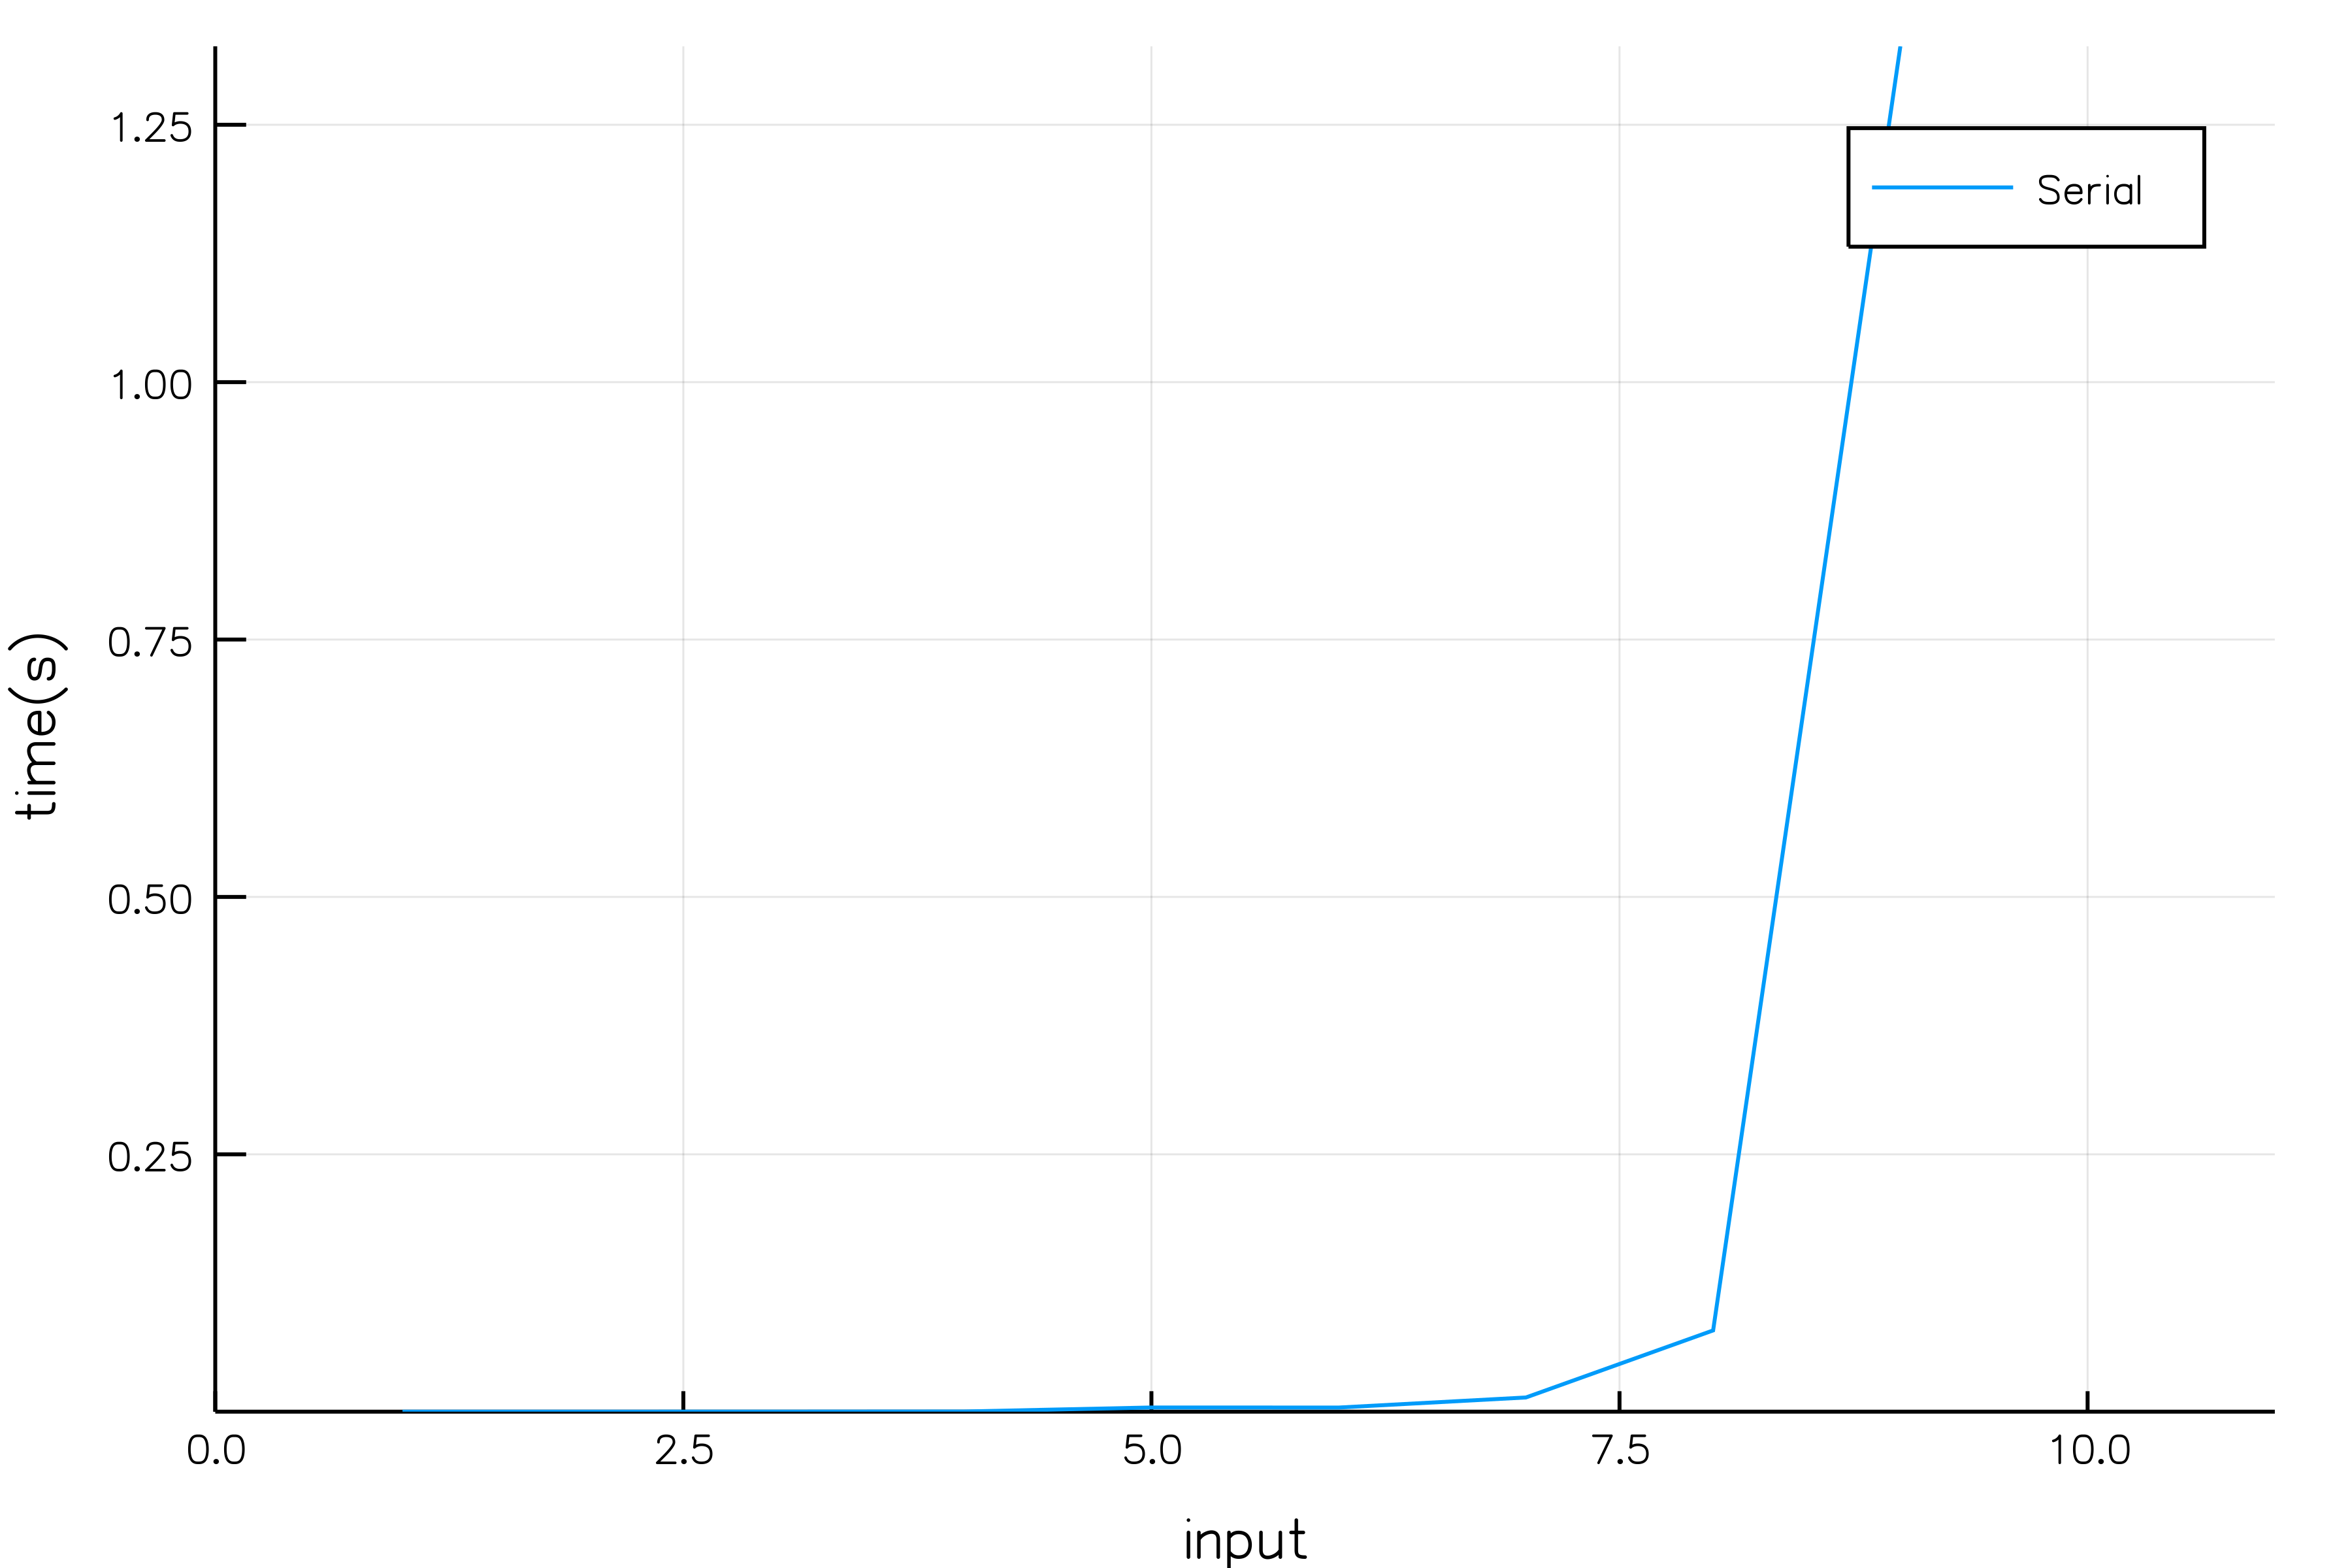
\includegraphics[width=13cm,scale=0.3]{struct.png}
\end{figure}
\newpage
\begin{verbatim}
pp=plot(yp,xaxis=''input'',yaxis=''time'',xlims=(0,length(input)+1),
       ylims=(0,maximum(y)+0.5),label=[''Parallel''],lw=2)
\end{verbatim}
\begin{figure}[ht!]
\centering
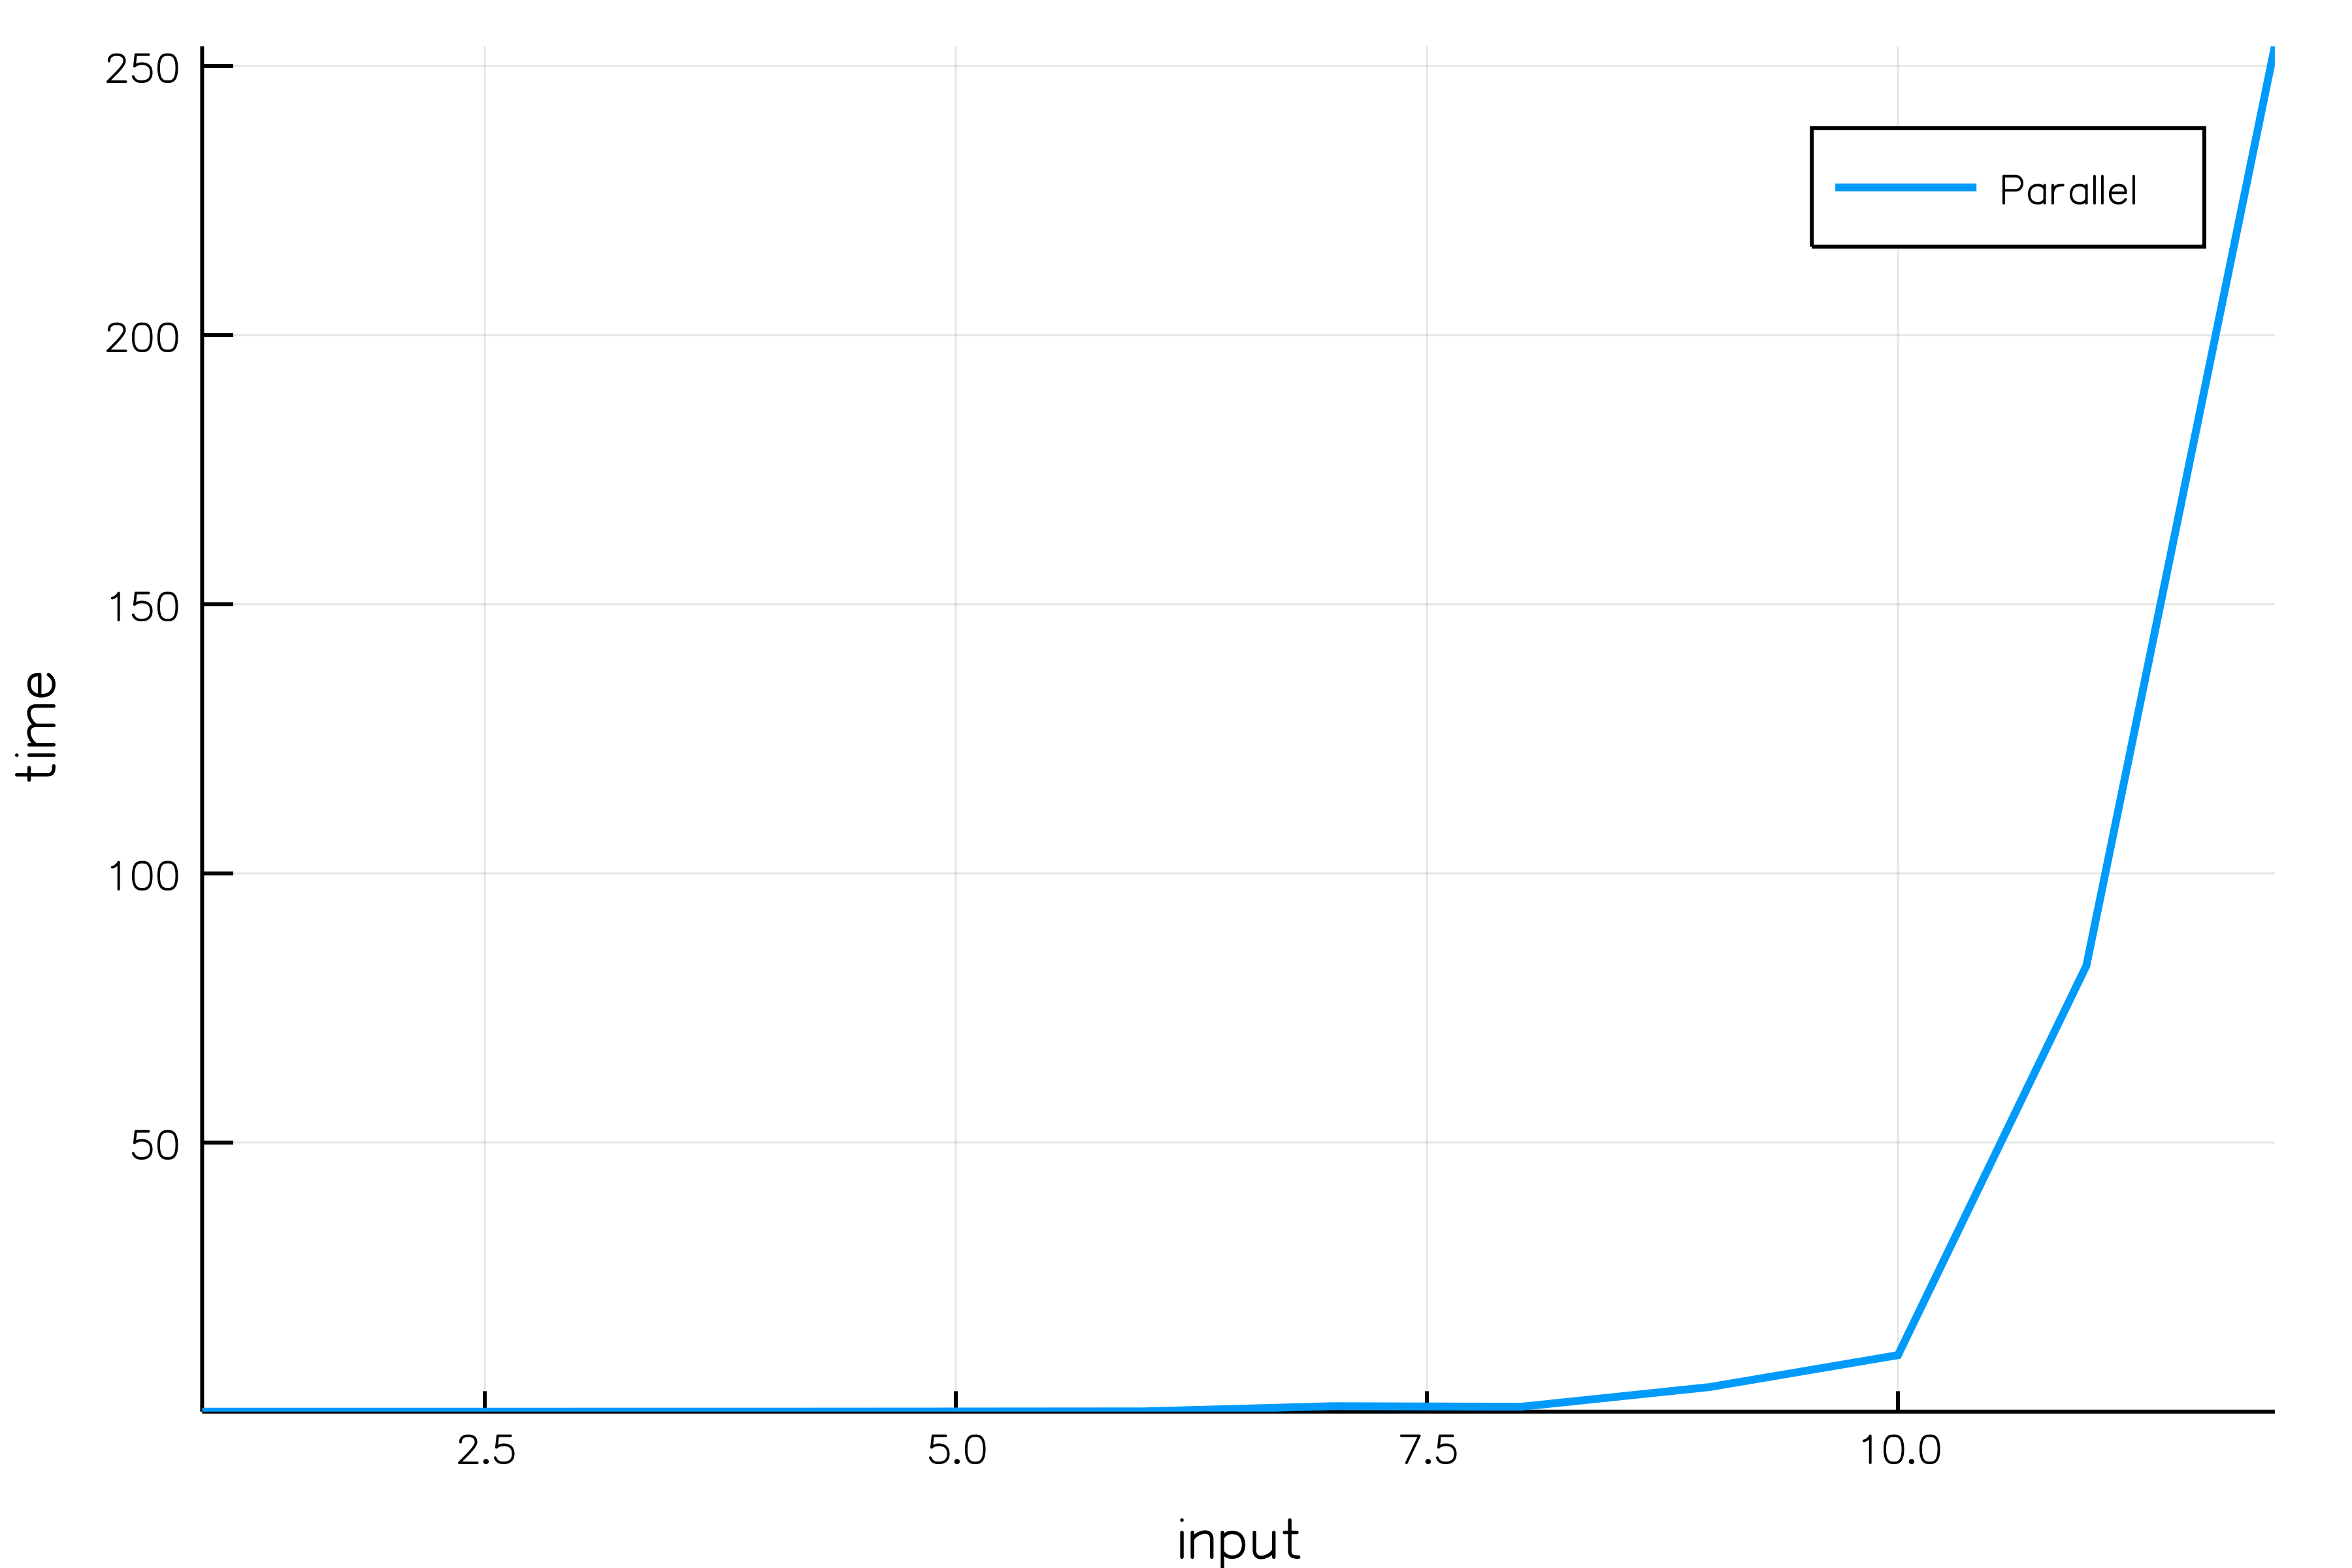
\includegraphics[width=11cm,scale=0.3]{pstruct.png}
\end{figure}
\newpage
\begin{verbatim}
yc=[y,yp]
pc=plot(yc,label=["Serial" "Parallel"])
\end{verbatim}
\begin{figure}[ht!]
\centering
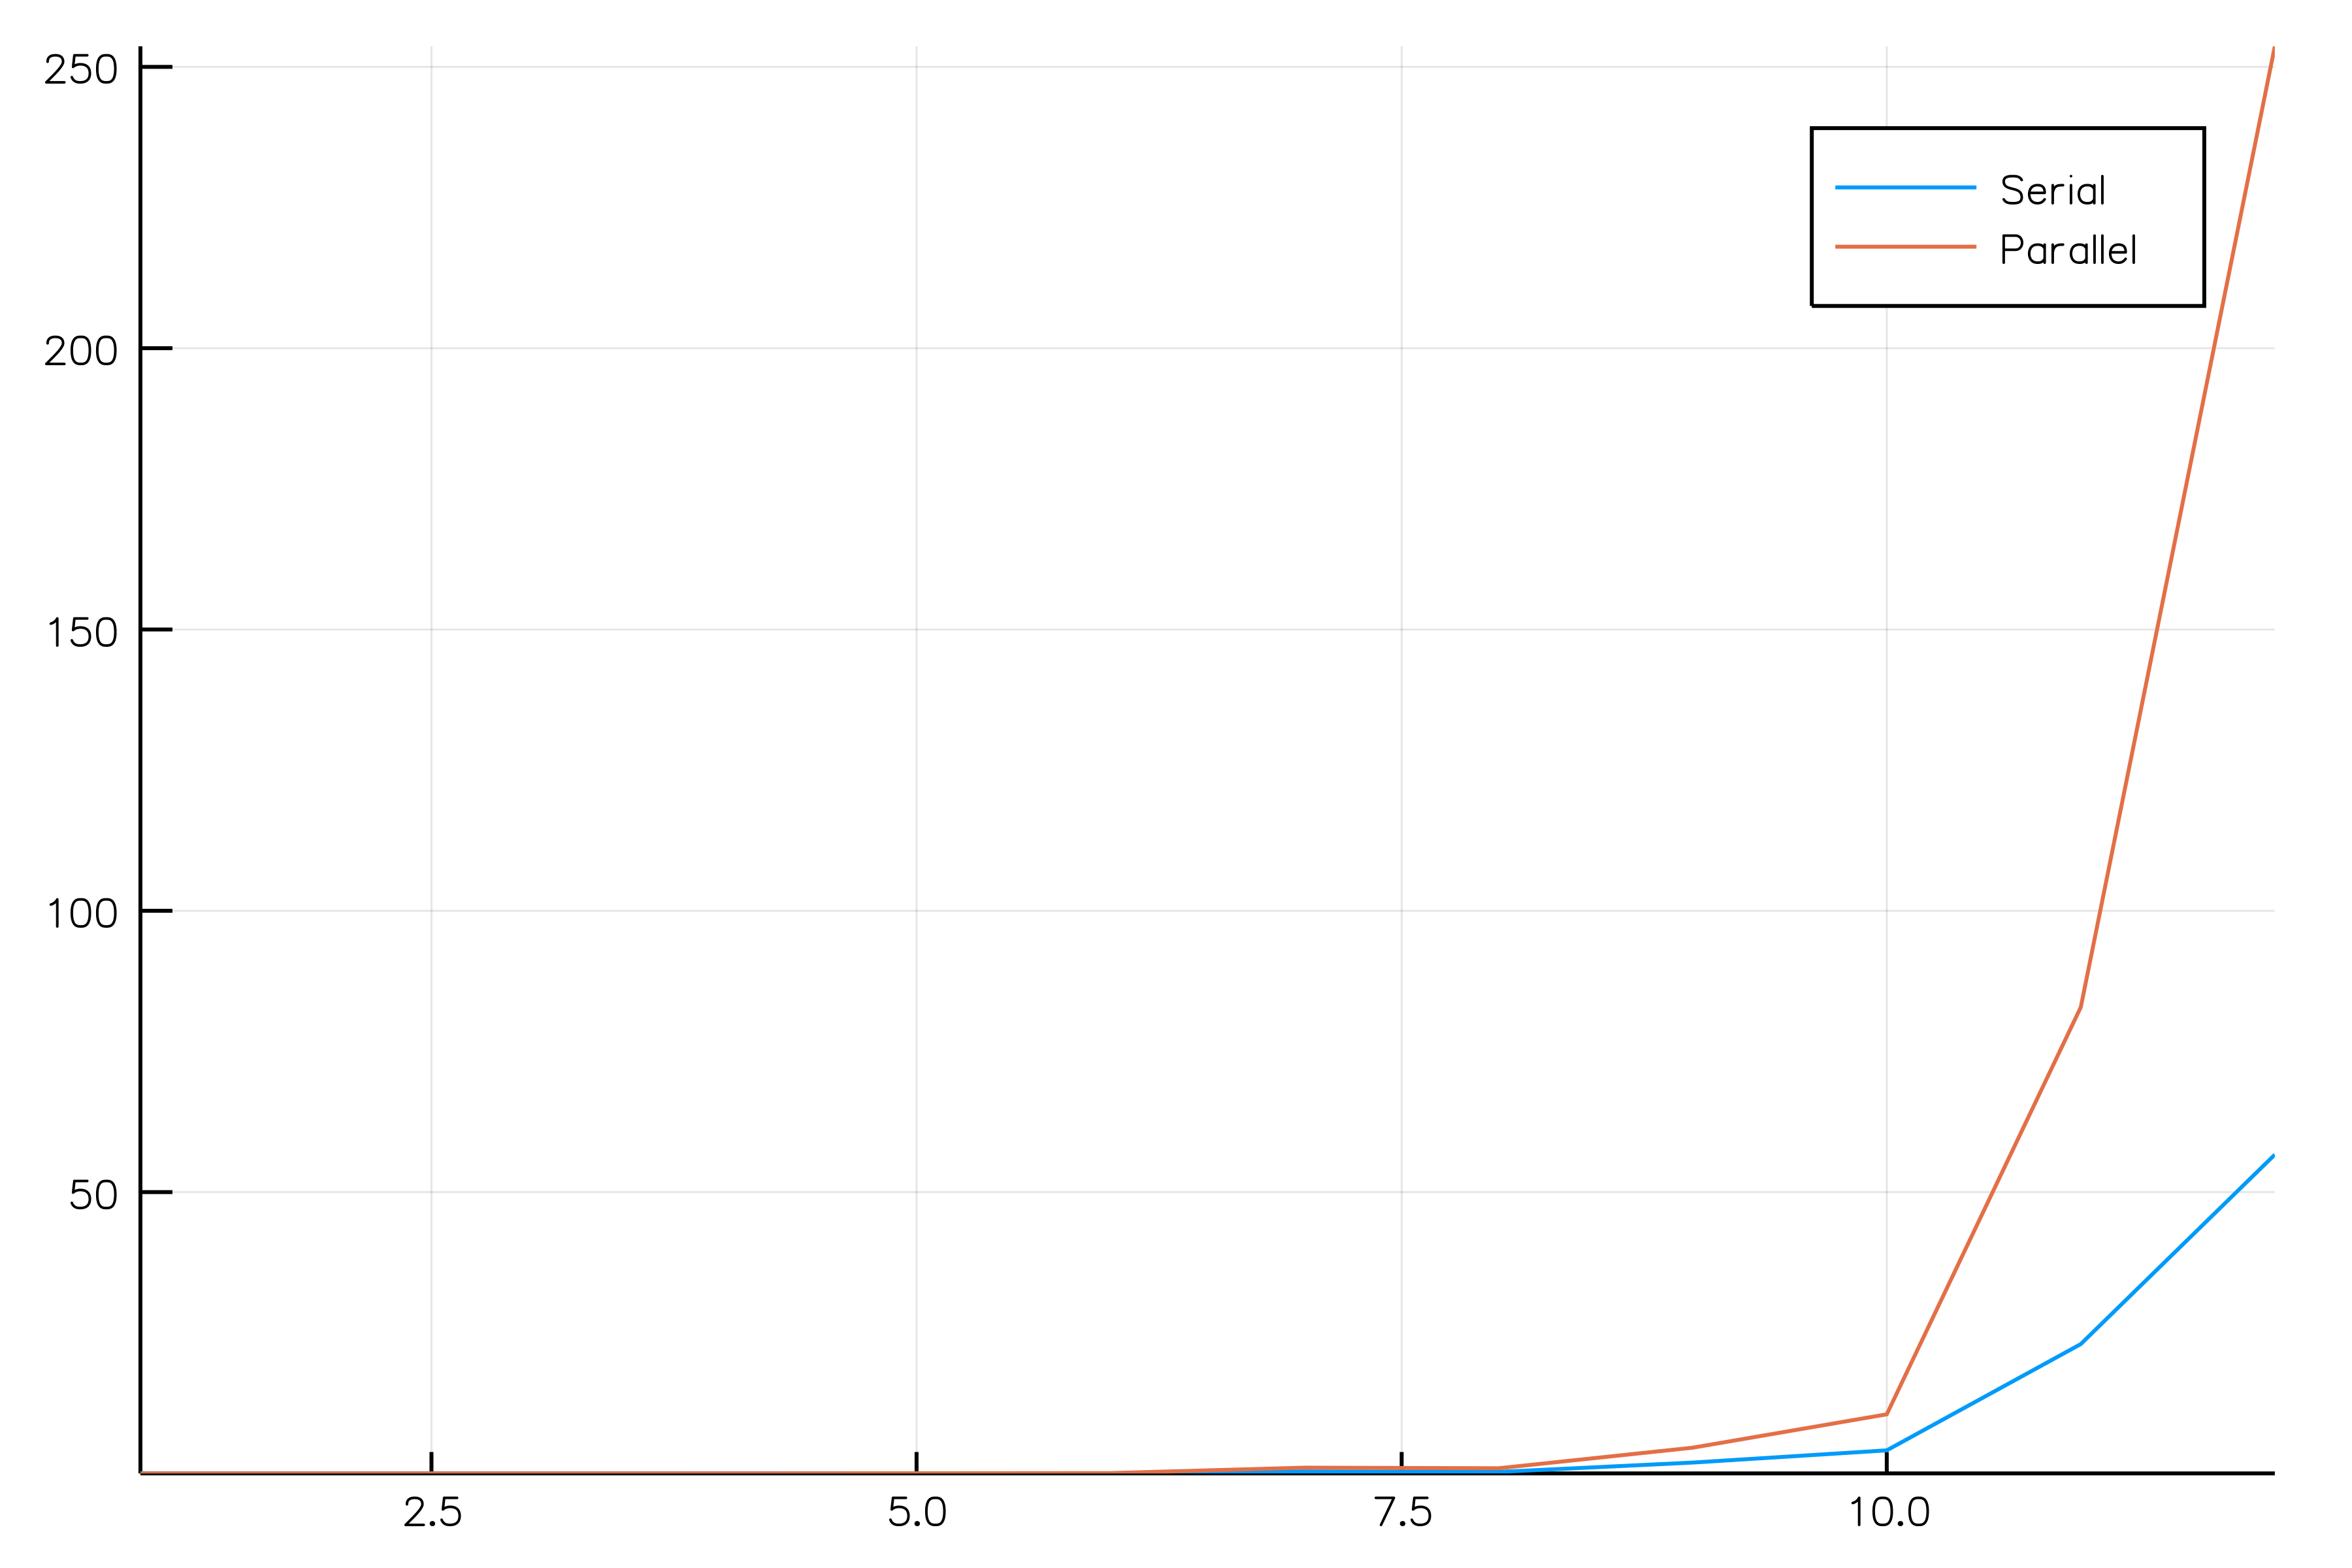
\includegraphics[width=11cm,scale=0.5]{compstruct.png}
\end{figure}
\newpage

\subsection{embedTraversal}
\subsubsection{Conversion}
\textbf{Python}
\begin{lstlisting}[language=Python,format=Julia]
def embedTraversal(cloned, obj,n,suffix):{
    for i in range(len(obj)):{
        if isinstance(obj[i],Model): {
            cloned.body += [obj[i]]}
        elif (isinstance(obj[i],tuple) or isinstance(obj[i],list)) and {?(len(obj[i])==2):
            V,EV = obj[i]
            V = [v+n*[0.0] for v in V]
            cloned.body  += [(V,EV)]}
        elif (isinstance(obj[i],tuple) or isinstance(obj[i],list)) and {?(len(obj[i])==3):
            V,FV,EV = obj[i]
            V = [v+n*[0.0] for v in V]
            cloned.body  += [(V,FV,EV)]}
        elif isinstance(obj[i],Mat): {
            mat = obj[i]
            d,d = mat.shape
            newMat = scipy.identity(d+n*1)
            for h in range(d-1): {
                for k in range(d-1): {
                    newMat[h,k] = mat[h,k]}
                newMat[h,d-1+n*1] = mat[h,d-1]}
            cloned.body  +=  [newMat.view(Mat)]}
        elif isinstance(obj[i],Struct):{
            newObj = Struct()
            newObj.box = hstack((obj[i].box, [n*[0],n*[0]]))
            newObj.name = obj[i].name+suffix
            newObj.category = obj[i].category
            cloned.body +=[embedTraversal(newObj, obj[i], n, suffix)]}
    return cloned
\end{lstlisting}
\textbf{Julia}
\begin{lstlisting}[language=Julia,format=Julia]
function embedTraversal(cloned,obj,n,suffix){
	for i in range(1,len(obj)){
		if isa(obj.body[i],Matrix){
			mat=obj.body[i]
			d,d=size(mat)
			newMat=eye(d+n*1)
			for h in range(1,d-1){
				for k in range(1,d-1){
					newMat[h,k]=mat[h,k]}
				end
				newMat[h,d-1+n*1]=mat[h,d-1]}
			end
			append!(cloned.body,newMat) }
		elseif (isa(obj.body[i],Tuple) ||isa(obj.body[i],Array))&& {? length(obj.body[i])==3 
			V,FV,EV=obj.body[i]
			dimadd=fill([0.0],n)
			for k in dimadd{
				for v in V{
					append!(v,k)}
				end}
			end
			append!(cloned.body,[(V,FV,EV)])}
		elseif (isa(obj.body[i],Tuple) ||isa(obj.body[i],Array))&& {?length(obj.body[i])==2 
			V,EV=deepcopy(obj.body[i])
			dimadd=fill([0.0],n)
			for k in dimadd{
				for v in V{
					append!(v,k)}
				end}
			end
			append!(cloned.body,[(V,EV)])}
		elseif isa(obj.body[i],Struct){
			newObj=Struct()
			newObj.box=hcat((obj.body[i].box,[fill([0],n),fill([0],n)]))
			newObj.category=obj.body[i].category
			append!(cloned.body,embedTraversal(newObj,obj.body[i],n,suffix))}
		end}
	end
	return cloned}
end
\end{lstlisting}
\subsubsection{Parallelization}
\begin{lstlisting}[language=Julia,format=Julia]
@everywhere function pembedTraversal(cloned,obj,n,suffix){
for i in range(1,len(obj)){
	      	 if (isa(obj.body[i],Matrix) || isa(obj.body[i],SharedArray)){
			mat=obj.body[i]
			d,d=size(mat)
			newMat=eye(d+n*1)
			@sync begin{
			for h in range(1,d-1){
				@async begin{
				       for k in range(1,d-1){
					   newMat[h,k]=mat[h,k]}
					end}
				end
				newMat[h,d-1+n*1]=mat[h,d-1]}
			end}
			end
			append!(cloned.body,newMat)}
		elseif (isa(obj.body[i],Tuple) ||isa(obj.body[i],Array))&& {?length(obj.body[i])==2 }
			V,EV=deepcopy(obj.body[i])
			dimadd=fill([0.0],n)
			@sync begin{
			      for k in dimadd{
			      	  @async begin{
				       for v in V{
				       	   append!(v,k)}
					end}
				end}
				end}
			end
			append!(cloned.body,[(V,EV)])}
		elseif (isa(obj.body[i],Tuple) ||isa(obj.body[i],Array))&&{? length(obj.body[i])==3}
			V,FV,EV=obj.body[i]
			dimadd=fill([0.0],n)
			@sync begin{
			      for k in dimadd{
			      	  @async begin{
				       for v in V{
				       	   append!(v,k)}
					end}
				end}
				end}
			end
			append!(cloned.body,[(V,FV,EV)])}		 
		elseif isa(obj.body[i],pStruct){
			newObj=pStruct()
			@async begin{
			newObj.box=hcat((obj.body[i].box,[fill([0],n),fill([0],n)]))
			newObj.category=obj.body[i].category
			append!(cloned.body,embedTraversal(newObj,obj.body[i],n,suffix))}
			end}
		end}
	end
	return cloned}
end
\end{lstlisting}
\subsubsection{Unit-Test}
\begin{lstlisting}[language=Julia,format=Julia]
square=([[0,0],[0,1],[1,0],[1,1]],[[0,1,2,3]])
x=Struct([square])

@testset "embedTraversal Tests" begin{
	@test length(embedTraversal(deepcopy(x),deepcopy(x),1,"New").body[2][1][1]){?==length(x.body[1][1][1])+1 }}
	#in this case n=1, but generally:
	# length(length(embedTraversal(x,x,1,"New")=length(x.body[1][1][1])+n
	@test length(embedTraversal(deepcopy(x),deepcopy(x),3,"New").body[2][1][1]){?==length(x.body[1][1][1])+3}}
	@test typeof(embedTraversal(deepcopy(x),deepcopy(x),1,"New"))==Struct	}	
end

square=([[0,0],[0,1],[1,0],[1,1]],[[0,1,2,3]])
x=pStruct([square])

@testset "pembedTraversal Tests" begin{
	@test length(pembedTraversal(deepcopy(x),deepcopy(x),1,"New").body[2][1][1]){?==length(x.body[1][1][1])+1 }}
	#in this case n=1, but generally:
	# length(length(embedTraversal(x,x,1,"New")=length(x.body[1][1][1])+n
	@test length(pembedTraversal(deepcopy(x),deepcopy(x),3,"New").body[2][1][1])=={?length(x.body[1][1][1])+3}}
	@test typeof(pembedTraversal(deepcopy(x),deepcopy(x),1,"New"))==pStruct	}	
end
\end{lstlisting}
\subsubsection{Results}
\begin{lstlisting}[language=Julia]
input=[1,10,50,10^2,5*10^2,10^3,5*10^3,10^4,5*10^4,10^5,5*10^5,10^6]
function timeEmbedTraversal(model,input)
	t=Array{Float64}(length(input))
	pt=Array{Float64}(length(input))
	for i in range(1,length(input))
	     structo=addn2D(input[i],model)
	     pstructo=pStruct(structo.body)
	     cloned=Struct()
	     cloned.box=hcat((structo.box,[fill([0],10),fill([0],10)]))	
	     cloned.name=string(object_id(cloned))
	     cloned.category=structo.category
	     cloned.dim=structo.dim+10
	     pcloned=pStruct()
	     pcloned.box=hcat((pstructo.box,[fill([0],10),fill([0],10)]))	
	     pcloned.name=string(object_id(pcloned))
	     pcloned.category=pstructo.category
	     pcloned.dim=pstructo.dim+10
	     embedTraversal(cloned,structo,10,"New")
	     pembedTraversal(pcloned,pstructo,10,"New")
	     t[i]=@elapsed embedTraversal(cloned,structo,10,"New")
	     pt[i]=@elapsed pembedTraversal(pcloned,pstructo,10,"New")
	end
	return t,pt
end
y,yp=timeEmbedTraversal(square,input)
p=plot(input,y,xaxis=''input'',yaxis=''time'',xlims=(0,length(input)+1),
       ylims=(0,maximum(y)+0.5), label=[''Serial''],lw=2)
\end{lstlisting}
\begin{figure}[ht!]
\centering
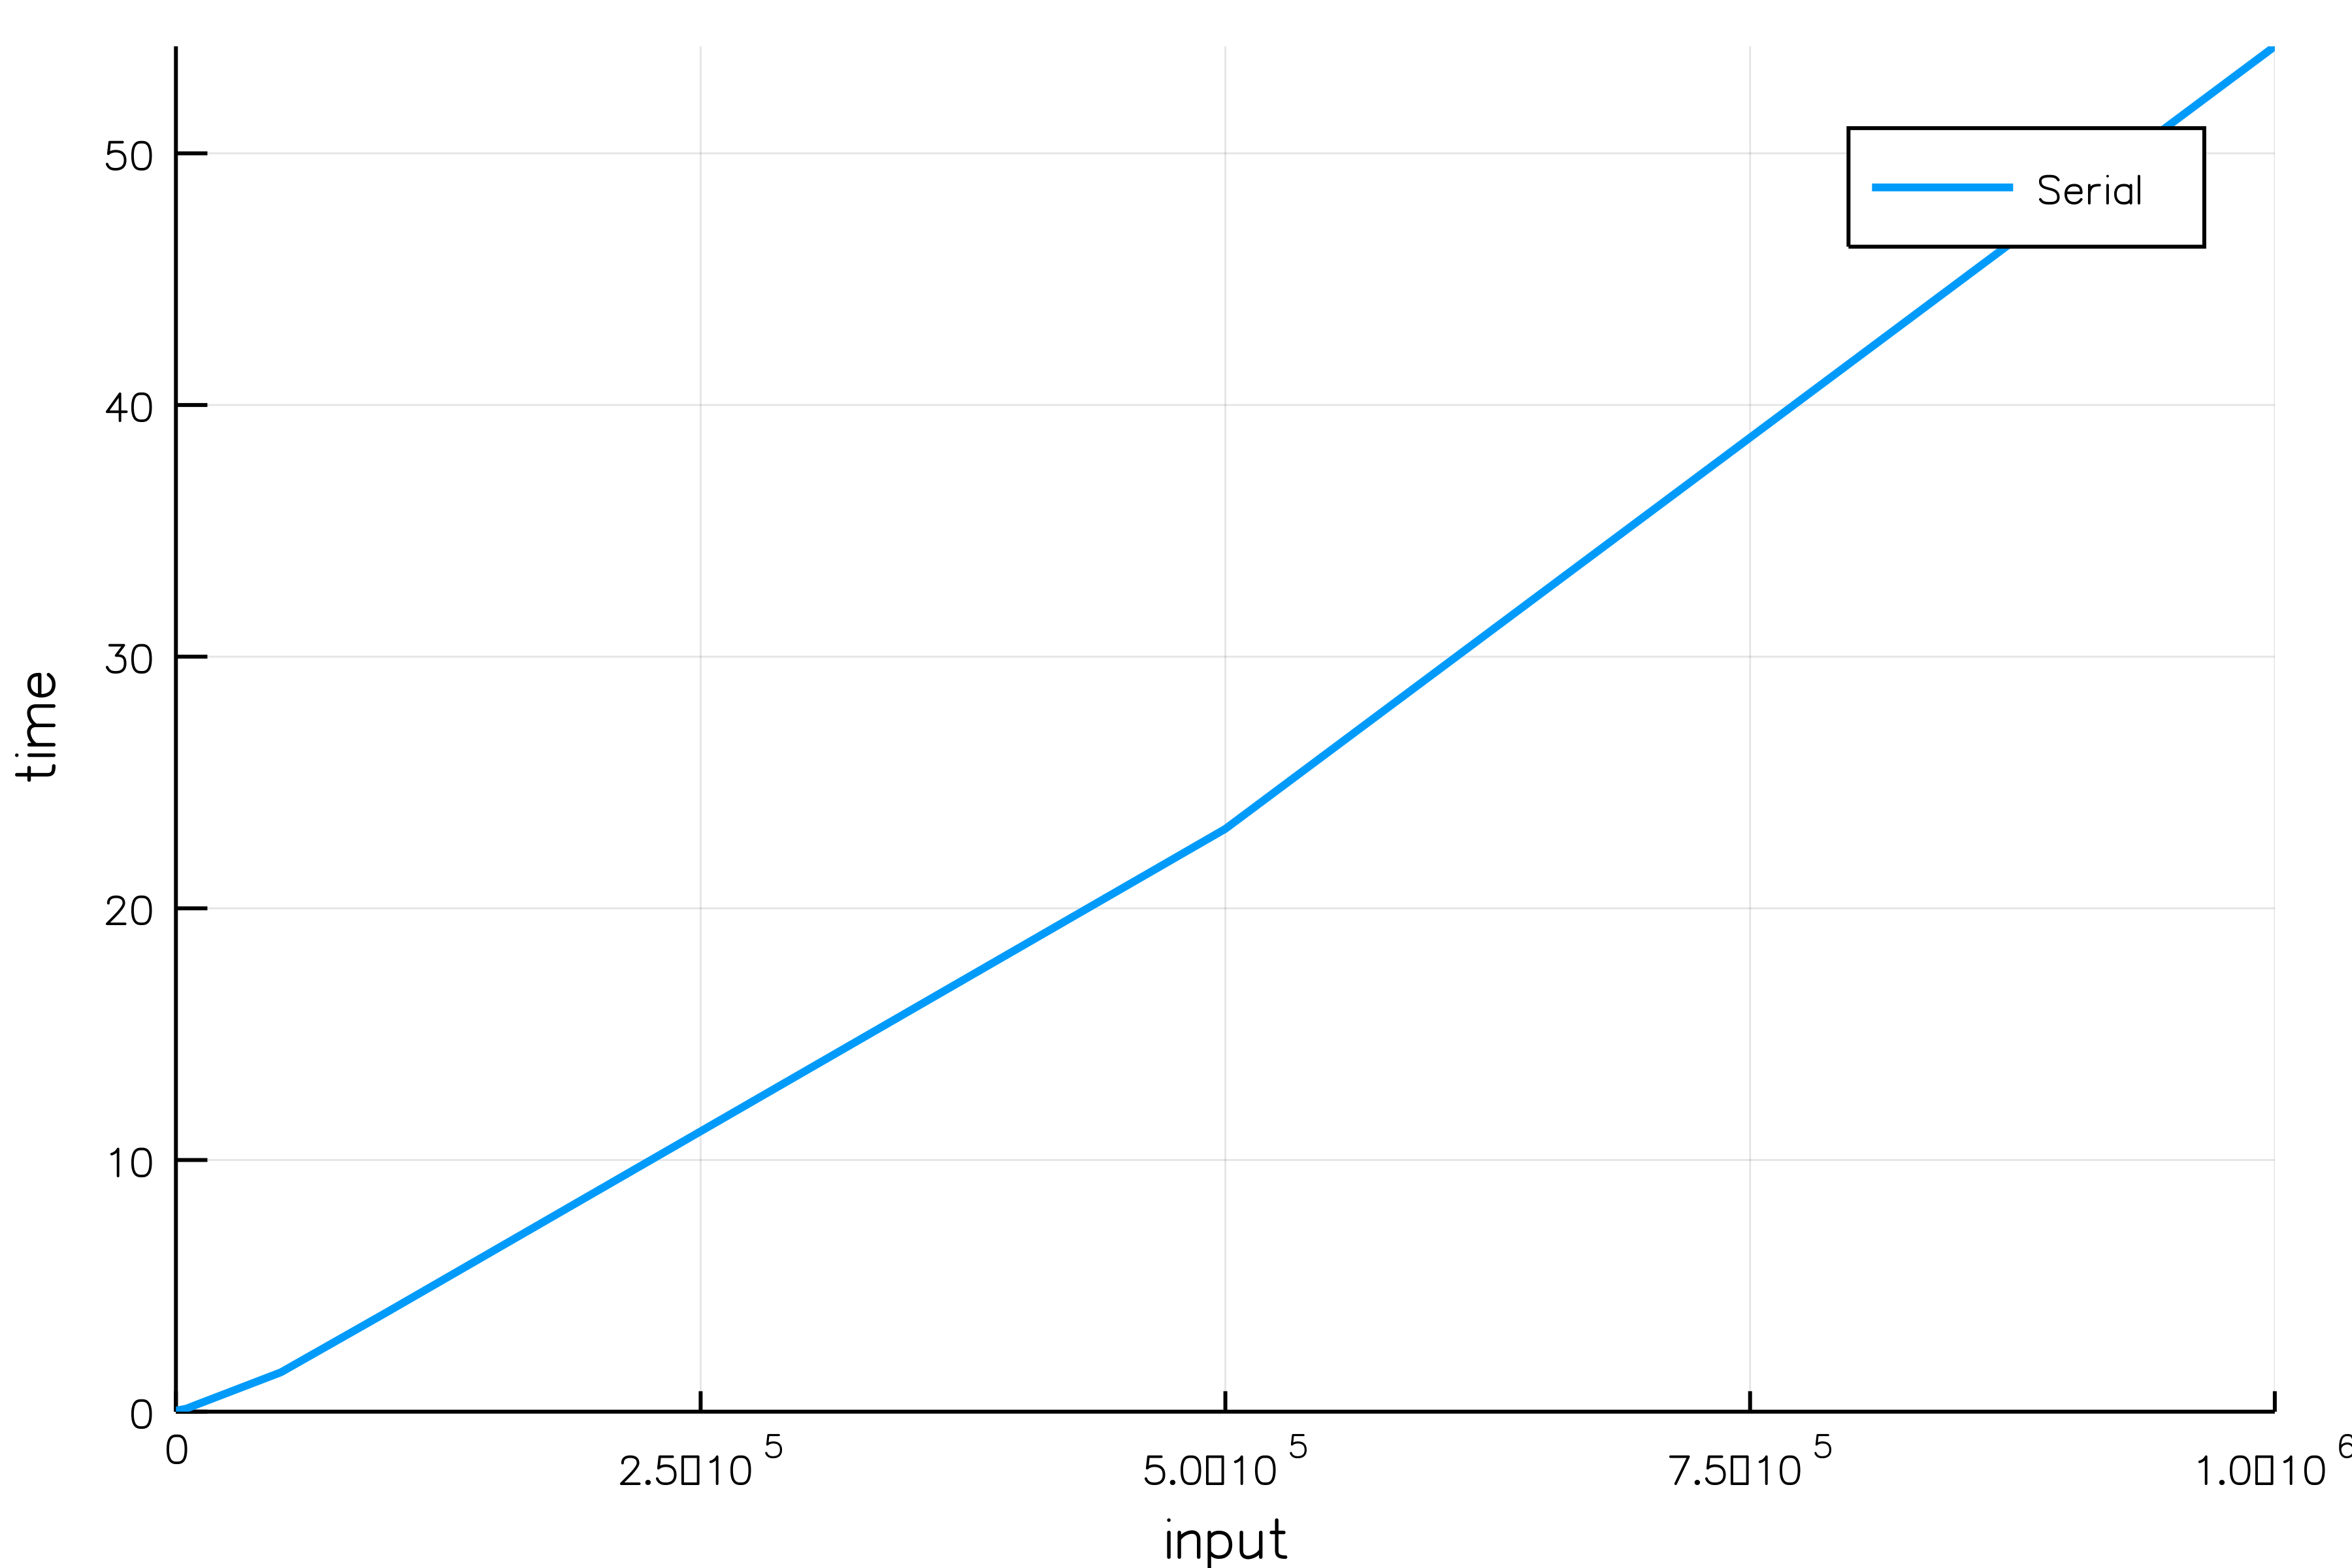
\includegraphics[width=13cm,scale=0.3]{embedtraversal.png}
\end{figure}
\newpage
\begin{verbatim}
pp=plot(input,yp,xaxis=''input'',yaxis=''time'',xlims=(0,length(input)+1),
       ylims=(0,maximum(y)+0.5),label=[''Parallel''],lw=2)
\end{verbatim}
\begin{figure}[ht!]
\centering
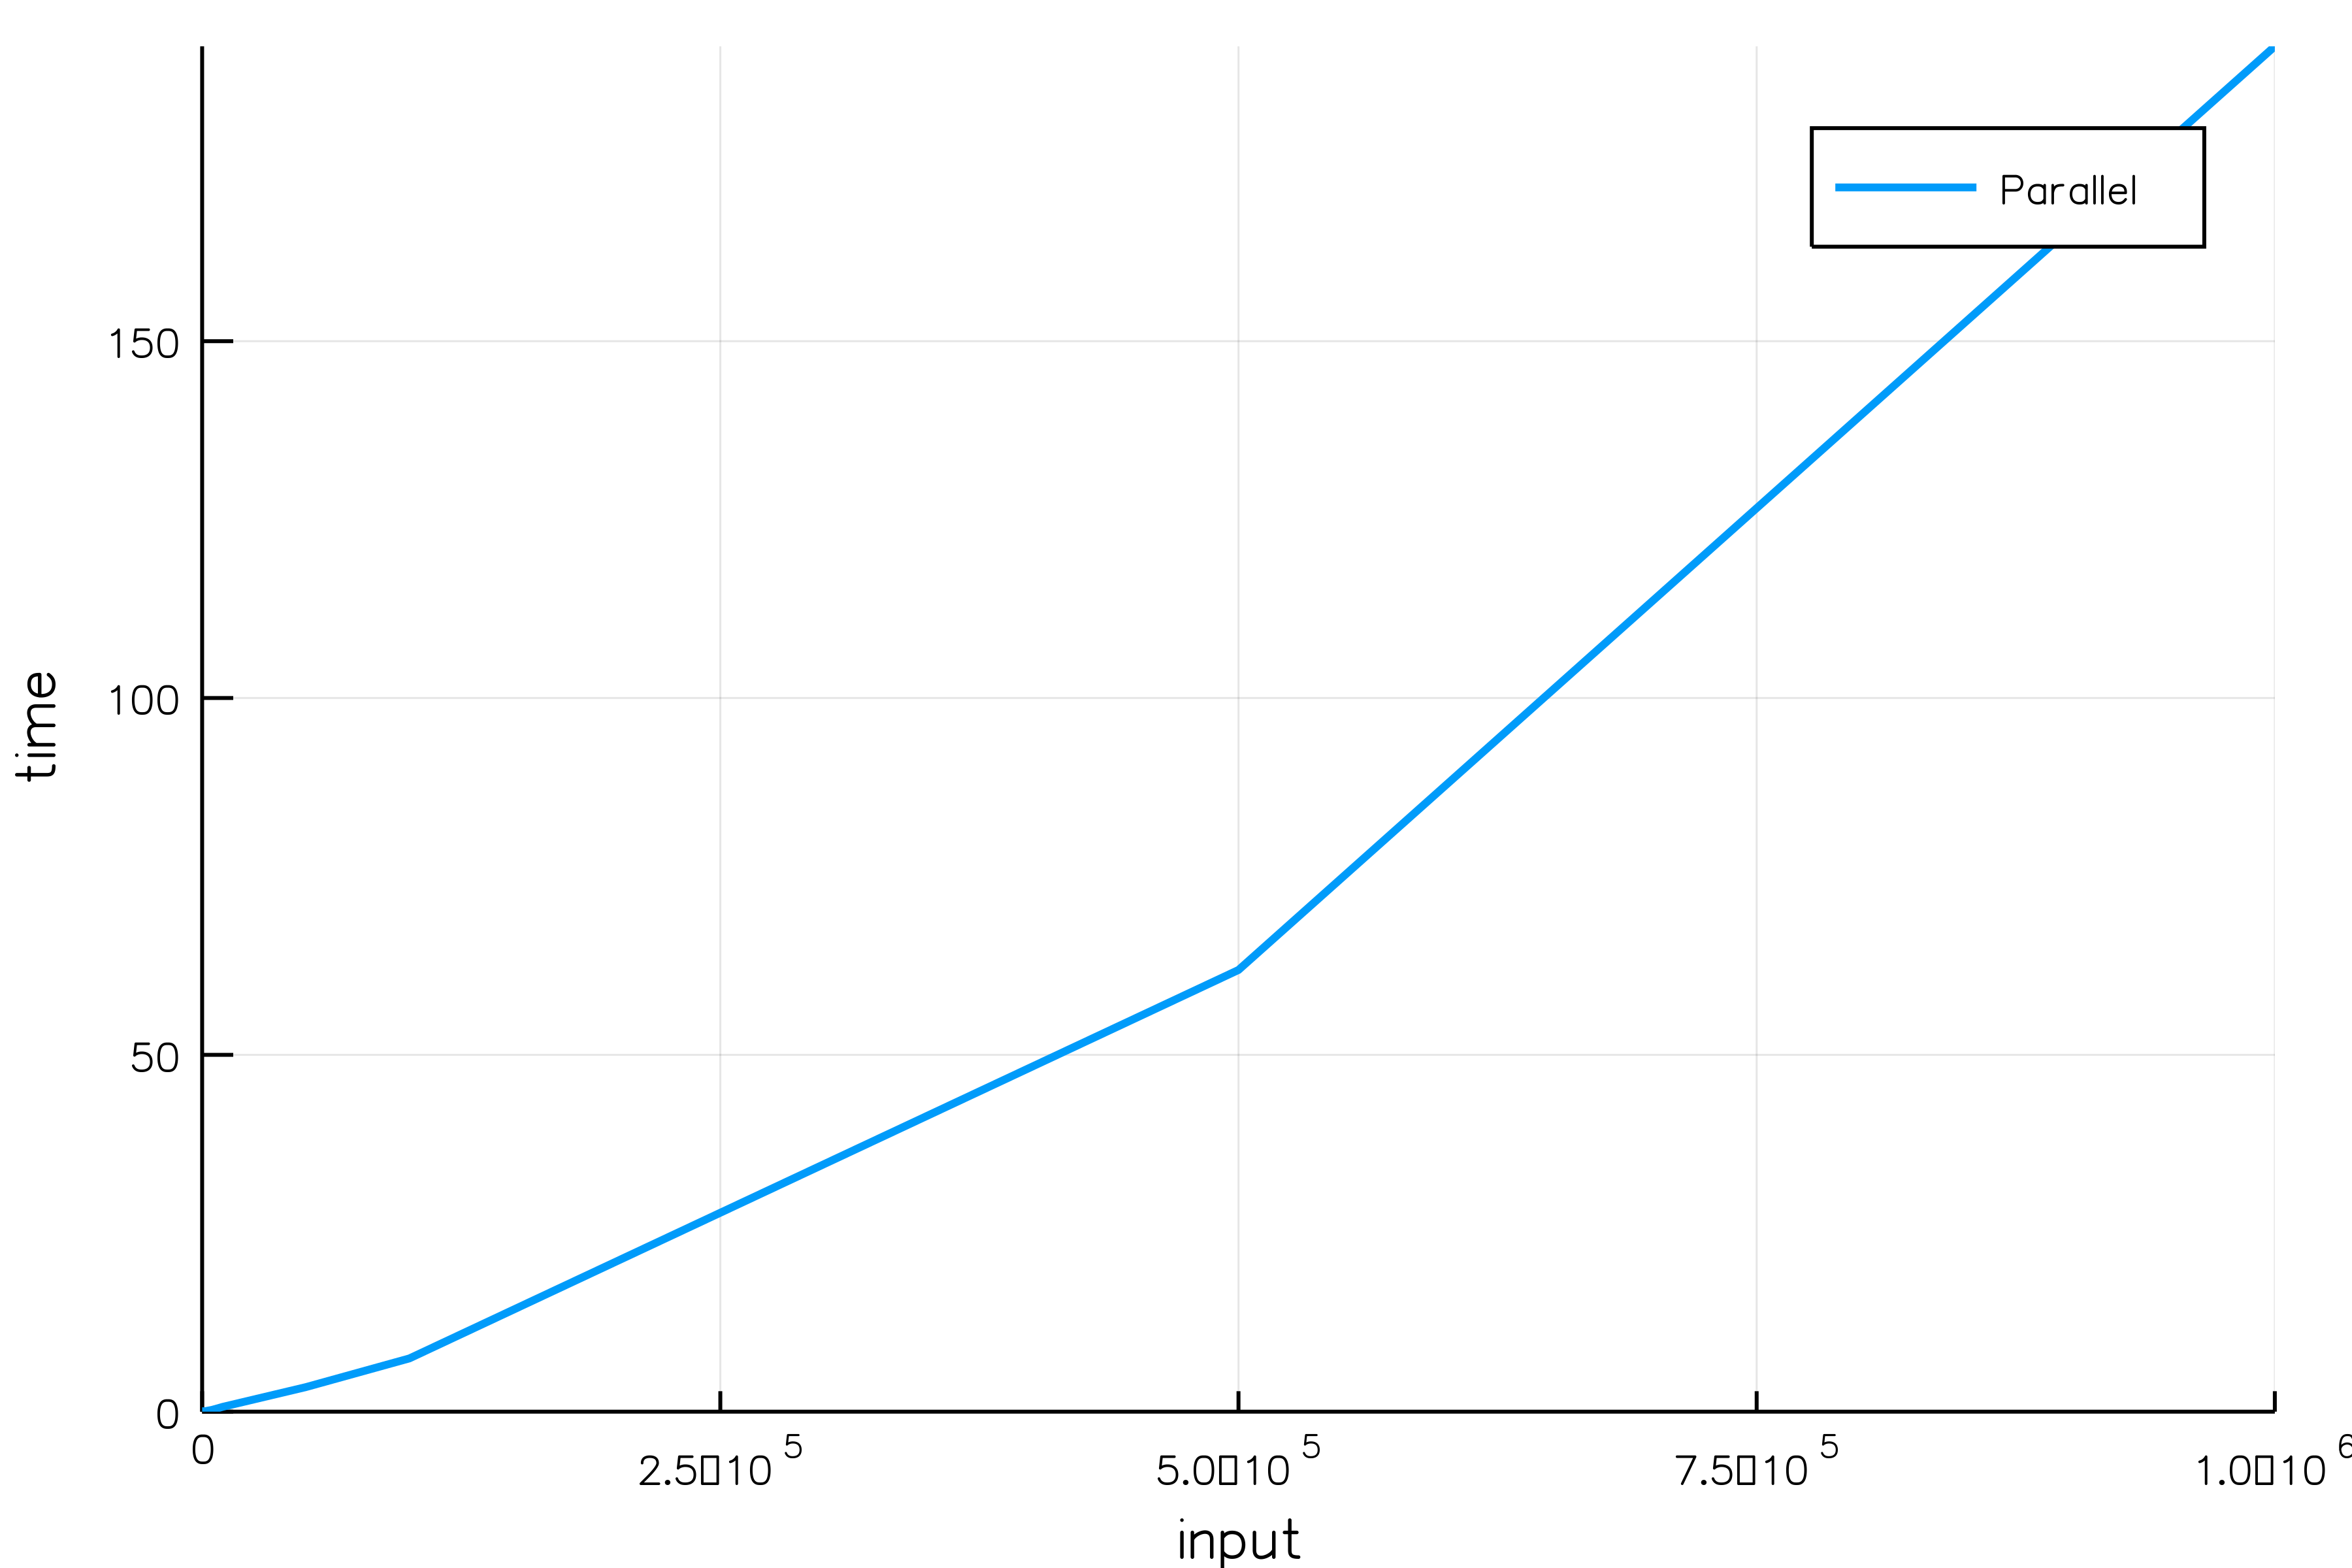
\includegraphics[width=11cm,scale=0.3]{pembedtraversal.png}
\end{figure}
\begin{verbatim}
yc=[y,yp]
pc=plot(input,yc,label=["Serial" "Parallel"])
\end{verbatim}
\begin{figure}[ht!]
\centering
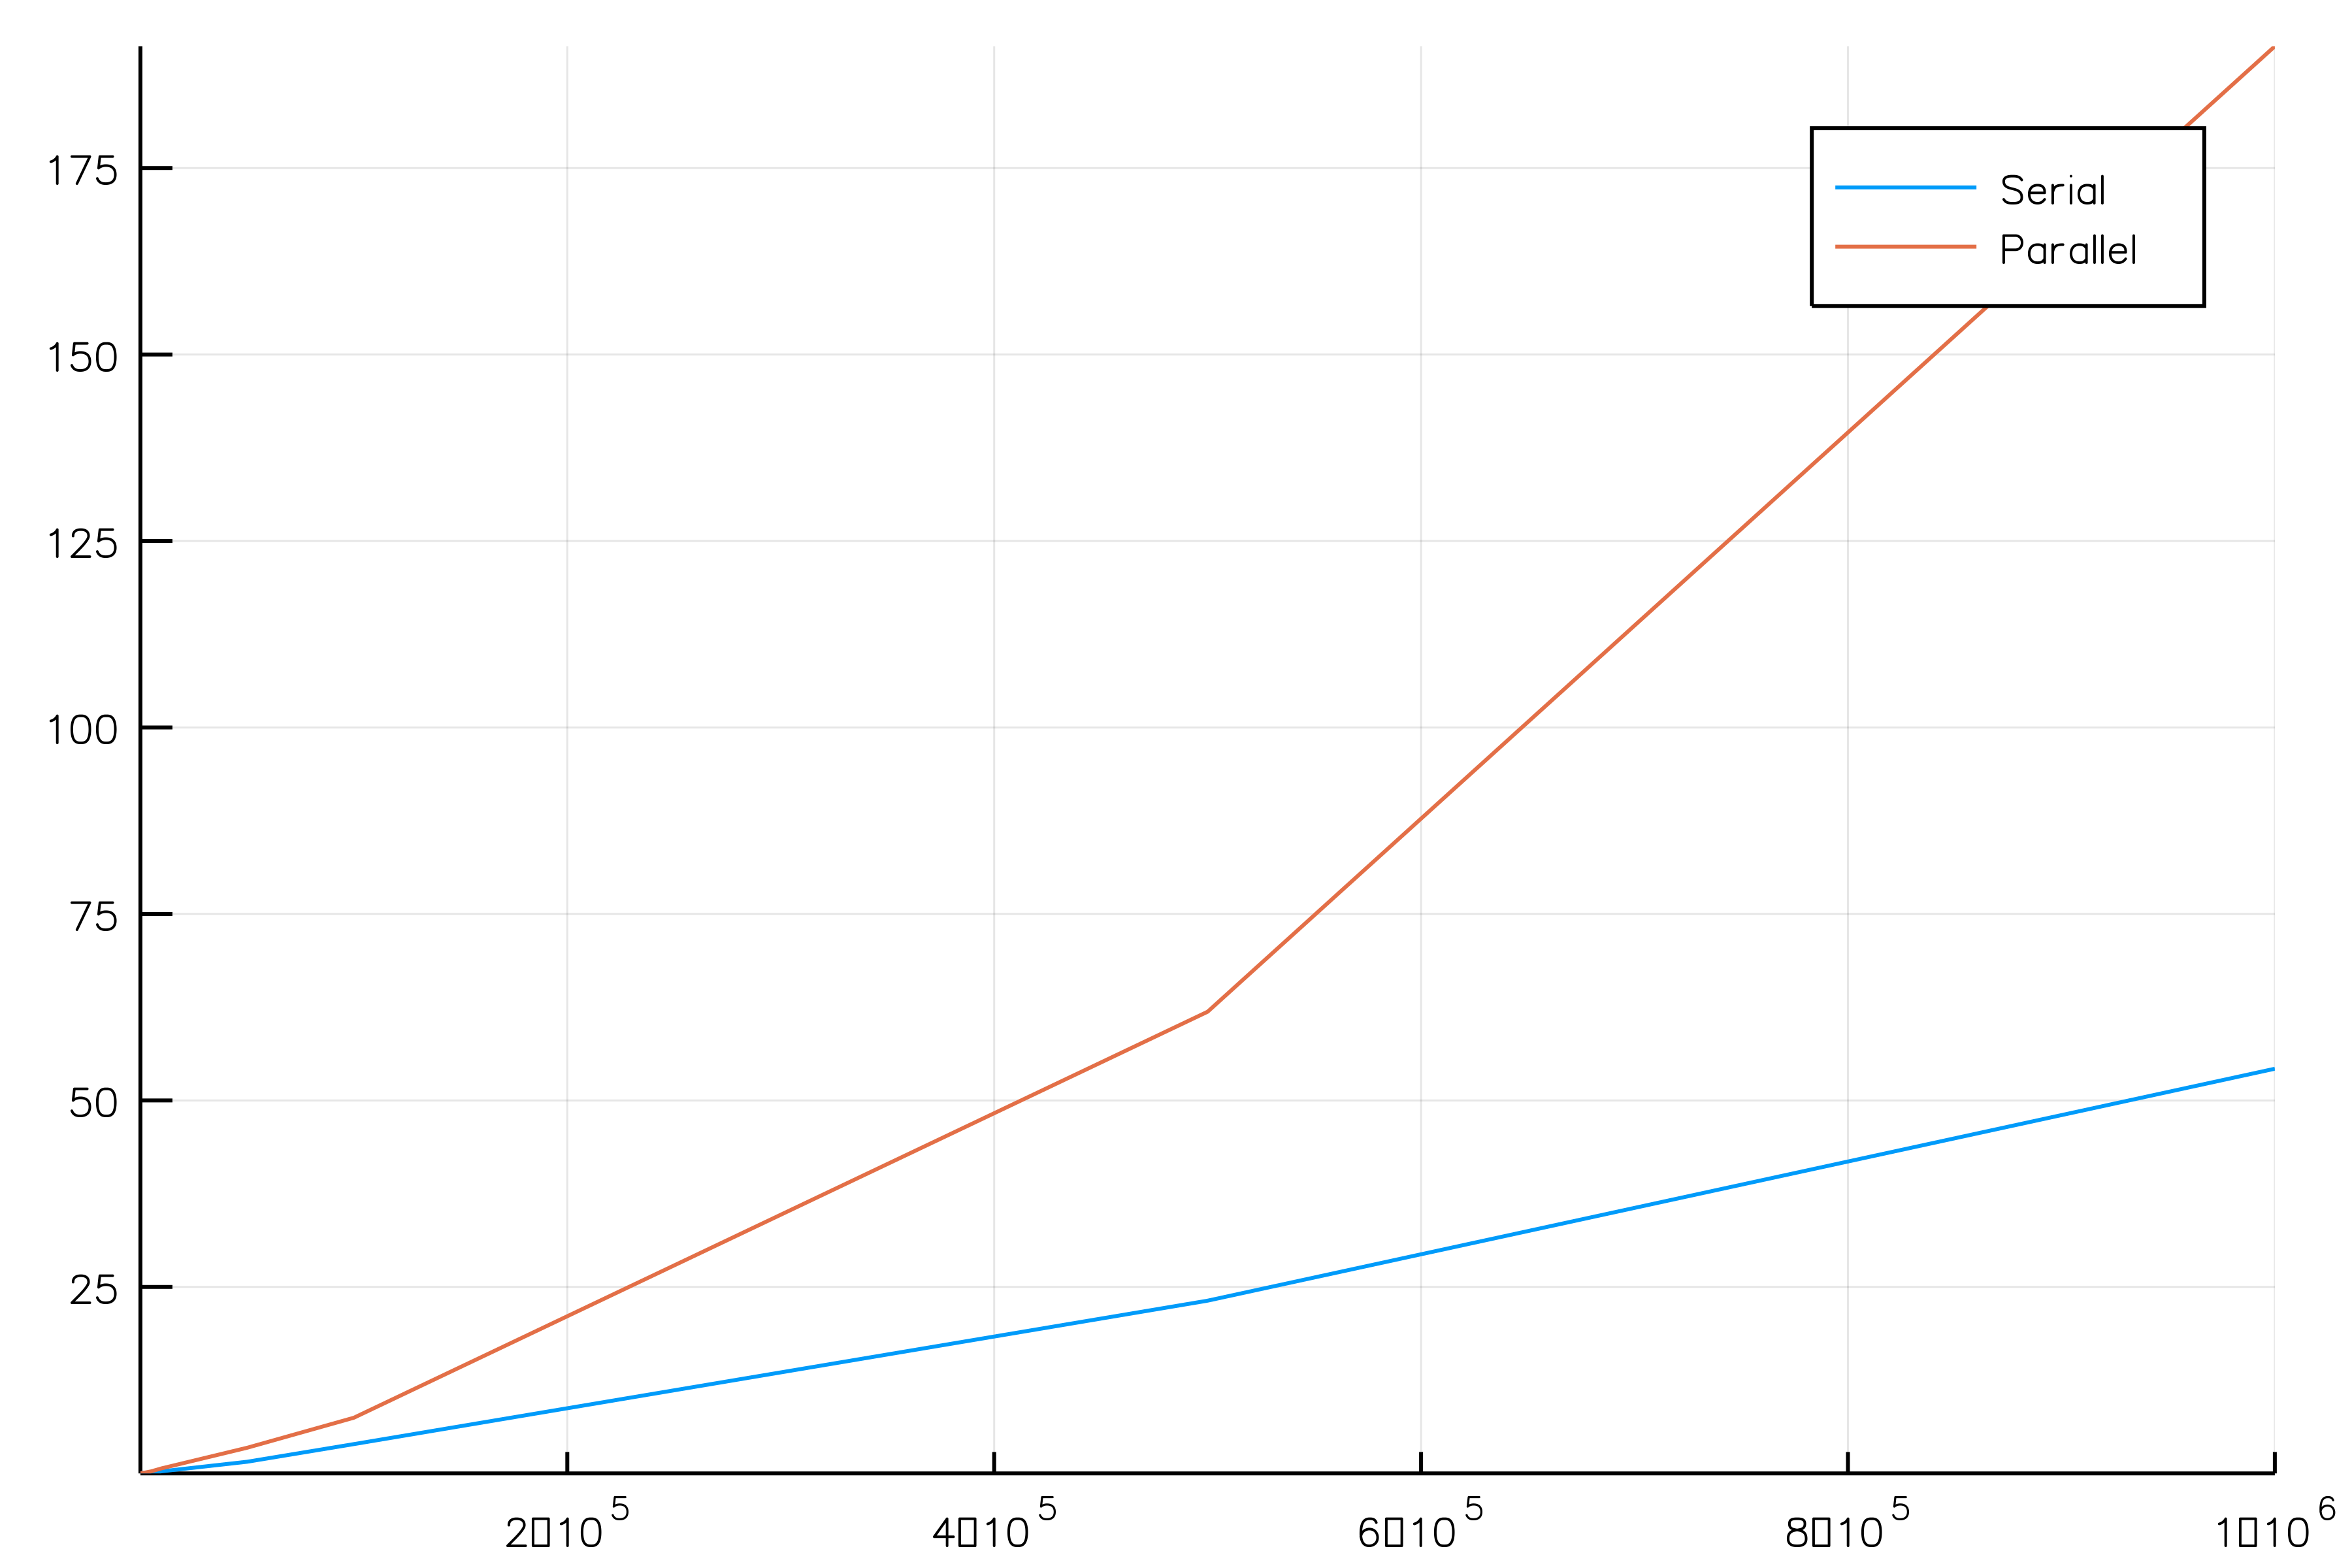
\includegraphics[width=11cm,scale=0.5]{compembedtraversal.png}
\end{figure}
\newpage
\subsection{embedStruct}
\subsubsection{Conversion}
\textbf{Python}
\begin{lstlisting}[language=Python,format=Julia]
def embedStruct(n):{
    def embedStruct0(struct,suffix="New"):{
        if n==0: {
            return struct, len(struct.box[0])}
        cloned = Struct()
        cloned.box = hstack((struct.box, [n*[0],n*[0]])).tolist()
        cloned.name = str(id(cloned))  #struct.name+suffix
        cloned.category = struct.category
        cloned.dim = struct.dim + n
        cloned = embedTraversal(cloned,struct,n,suffix) 
        return cloned}
    return embedStruct0
\end{lstlisting}
\textbf{Julia}
\begin{lstlisting}[language=Julia,format=Julia]
function embedStruct(n){
	function embedStruct0(self,suffix="New"){
		if n==0{
			return self, length(self.box[1])}
		end
		cloned=Struct()
		cloned.box=hcat((self.box,[fill([0],n),fill([0],n)]))	
		cloned.name=string(object_id(cloned))
		cloned.category=self.category
		cloned.dim=self.dim+n
		cloned=embedTraversal(cloned,self,n,suffix)
		return cloned}
	end
	return embedStruct0}
end
\end{lstlisting}
\subsubsection{Parallelization}
\begin{lstlisting}[language=Julia,format=Julia]
@everywhere function pembedStruct(n){
	function pembedStruct0(self,suffix="New"){
		if n==0{
			return self, length(self.box[1])}
		end
		cloned=pStruct()
		cloned.box=hcat((self.box,[fill([0],n),fill([0],n)]))	
		cloned.name=string(object_id(cloned))
		cloned.category=self.category
		cloned.dim=self.dim+n
		cloned=pembedTraversal(cloned,self,n,suffix)
		return cloned}
	end
	return pembedStruct0}
end
\end{lstlisting}
\subsubsection{Unit-Test}\begin{lstlisting}[language=Julia,format=Julia]
square=([[0,0],[0,1],[1,0],[1,1]],[[0,1,2,3]])
x=Struct([square])	
@testset "embedStruct Tests" begin{
	@test length(embedStruct(1)(x).body[1][1][1])==length(x.body[1][1][1])+1 
	#in this case n = 1, but generally: 
	#length(embedStruct(n)(x).body[1][1][1])=length(x.body[1][1][1])+n
	@test length(embedStruct(3)(x).body[1][1][1])==length(x.body[1][1][1])+3
	@test typeof(embedStruct(1)(x))==Struct	}	
end

square=([[0,0],[0,1],[1,0],[1,1]],[[0,1,2,3]])
x=pStruct([square])	
@testset "pembedStruct Tests" begin{	
	@test length(pembedStruct(1)(x).body[1][1][1])==length(x.body[1][1][1])+1 
	#in this case n = 1, but generally: 
	#length(embedStruct(n)(x).body[1][1][1])=length(x.body[1][1][1])+n
	@test length(pembedStruct(3)(x).body[1][1][1])==length(x.body[1][1][1])+3
	@test typeof(pembedStruct(1)(x))==pStruct	}	
end
\end{lstlisting}
\subsubsection{Results}
\begin{lstlisting}[language=Julia]
function timeEmbedStruct(n,model,input)
	t=Array{Float64}(length(input))
	pt=Array{Float64}(length(input))
	for i in range(1,length(input))
	    structo=addn2D(input[i],model)
	     pstructo=pStruct(structo.body)
	    embedStruct(n)(structo)
	    pembedStruct(n)(pstructo)
	     t[i]=@elapsed embedStruct(n)(structo)
	    pt[i]=@elapsed pembedStruct(n)(pstructo)
	end
	return t,pt
end

y,yp=timeEmbedStruct(10,square,input)
p=plot(input,y,xaxis=''input'',yaxis=''time'',xlims=(0,length(input)+1),
       ylims=(0,maximum(y)+0.5), label=[''Serial''],lw=2)
\end{lstlisting}
\begin{figure}[ht!]
\centering
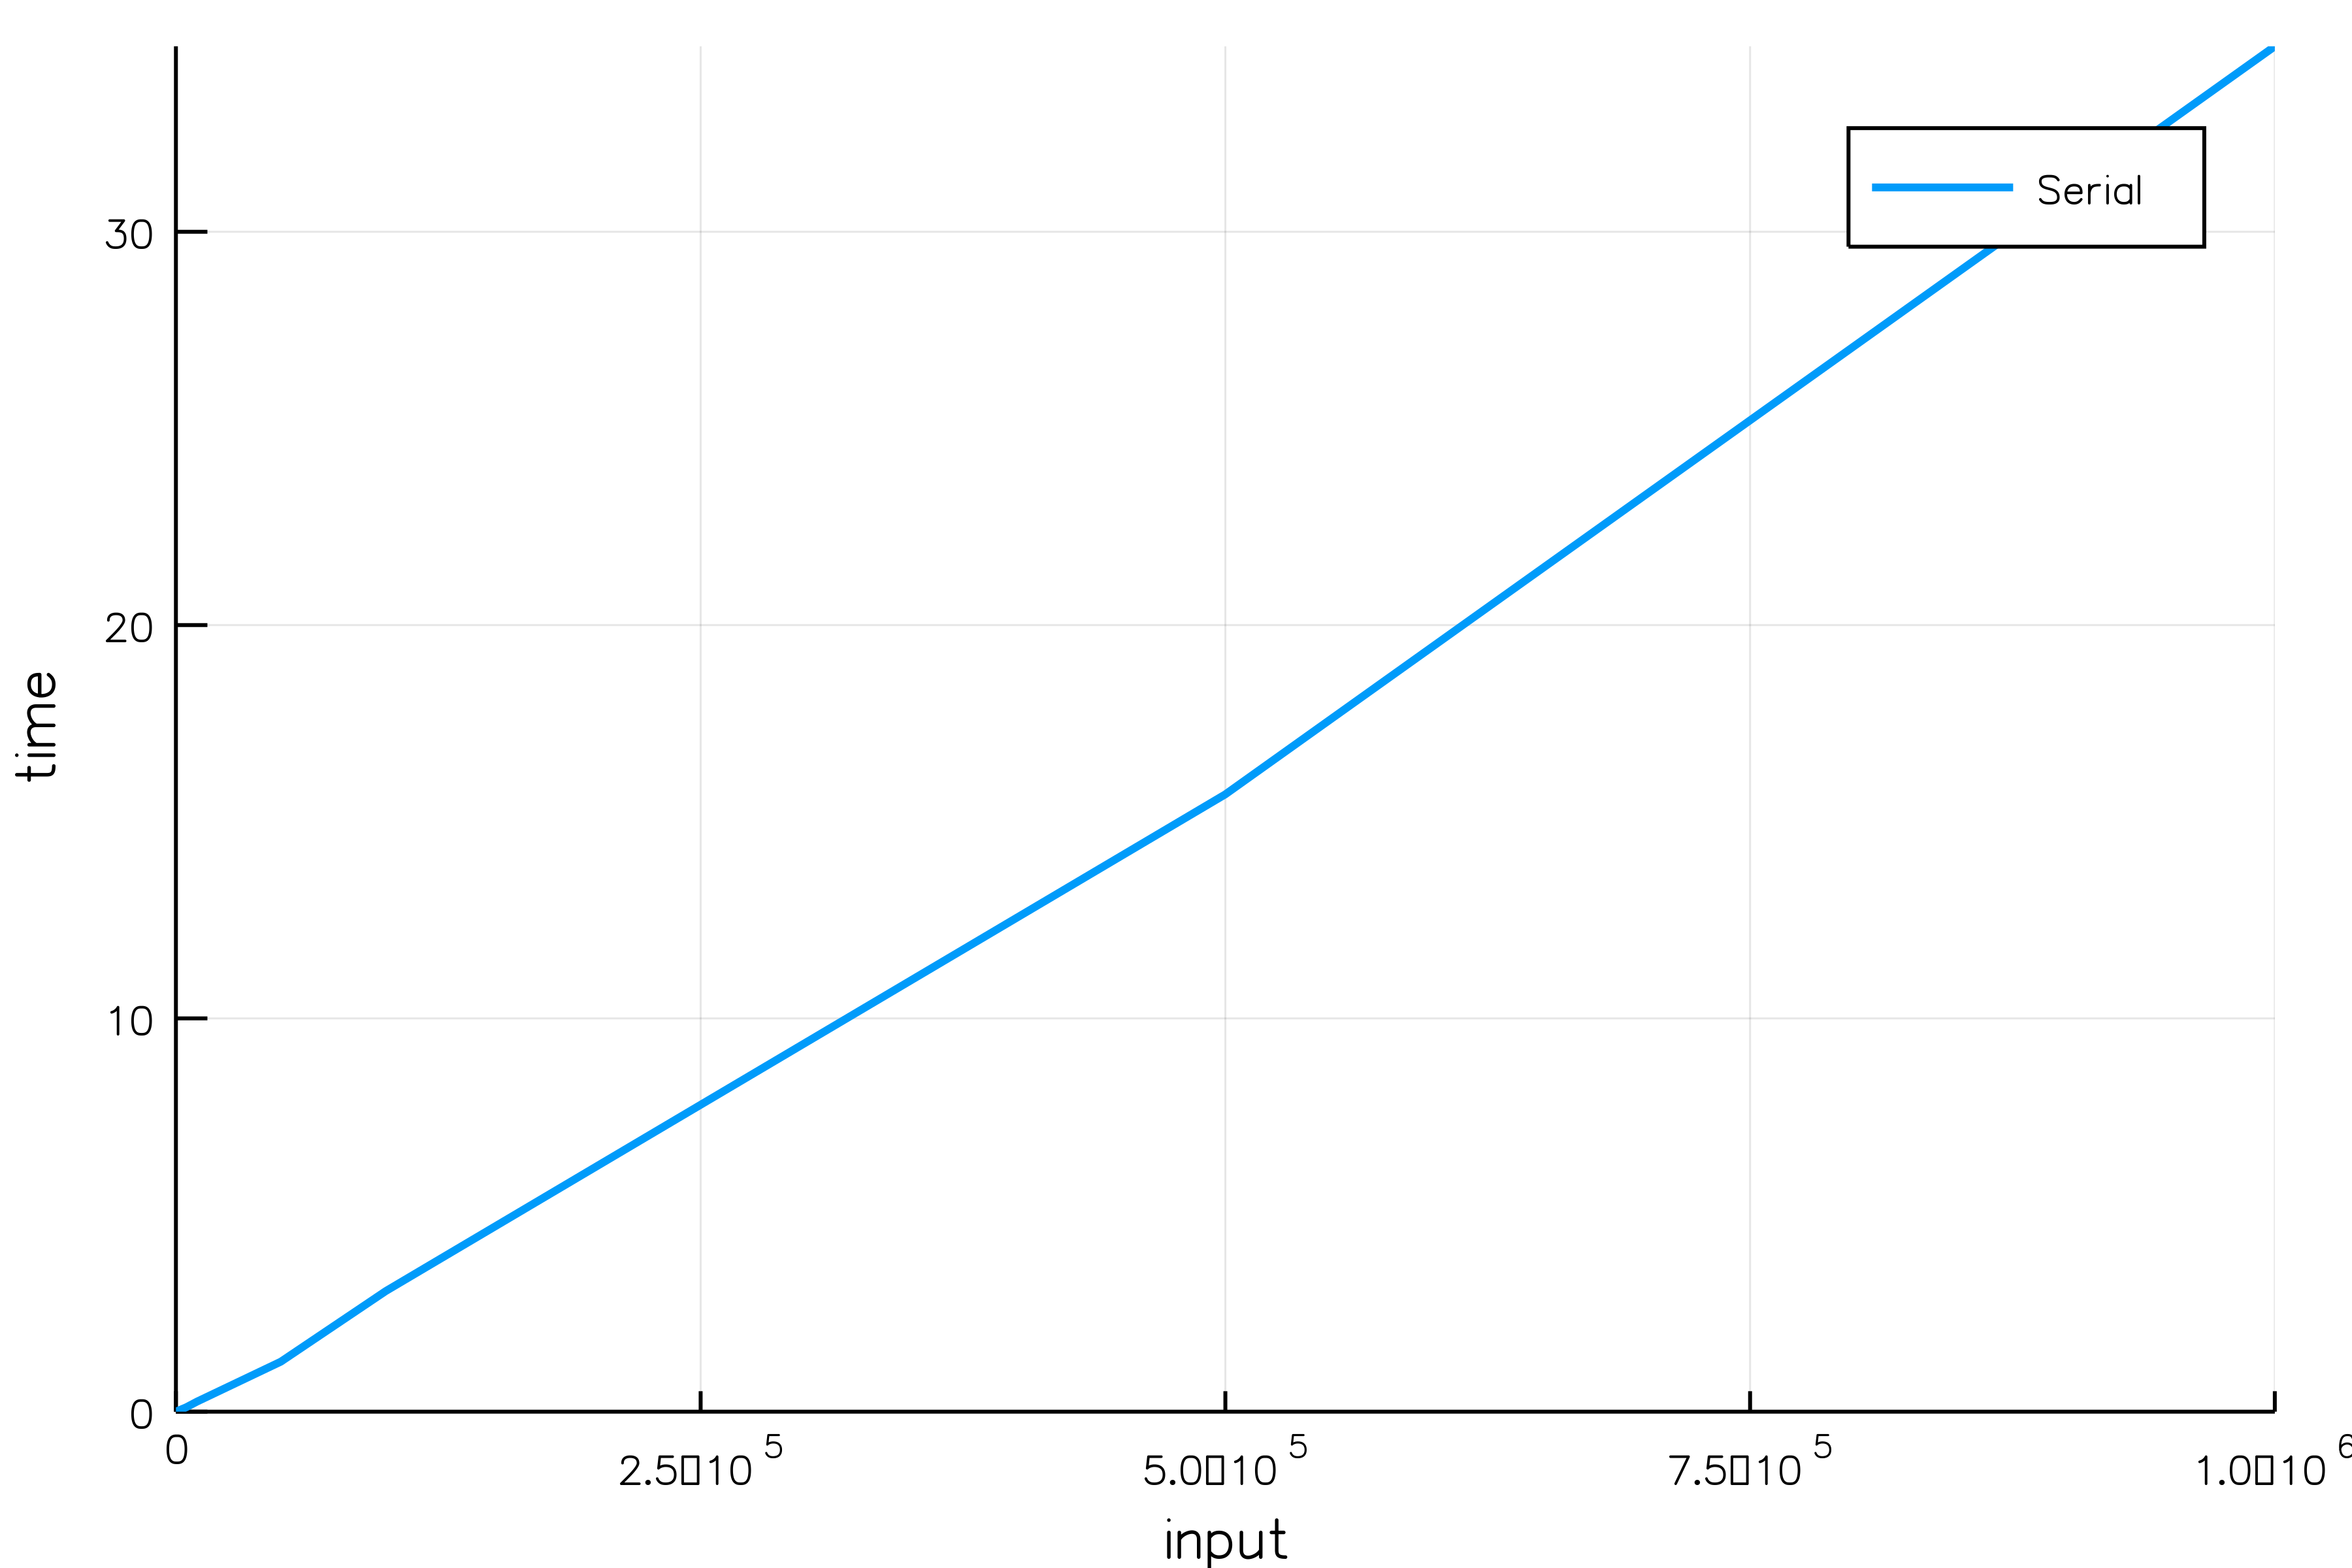
\includegraphics[width=13cm,scale=0.3]{embedStruct.png}
\end{figure}
\newpage
\begin{verbatim}
pp=plot(input,yp,xaxis=''input'',yaxis=''time'',xlims=(0,length(input)+1),
       ylims=(0,maximum(y)+0.5),label=[''Parallel''],lw=2)
\end{verbatim}
\begin{figure}[ht!]
\centering
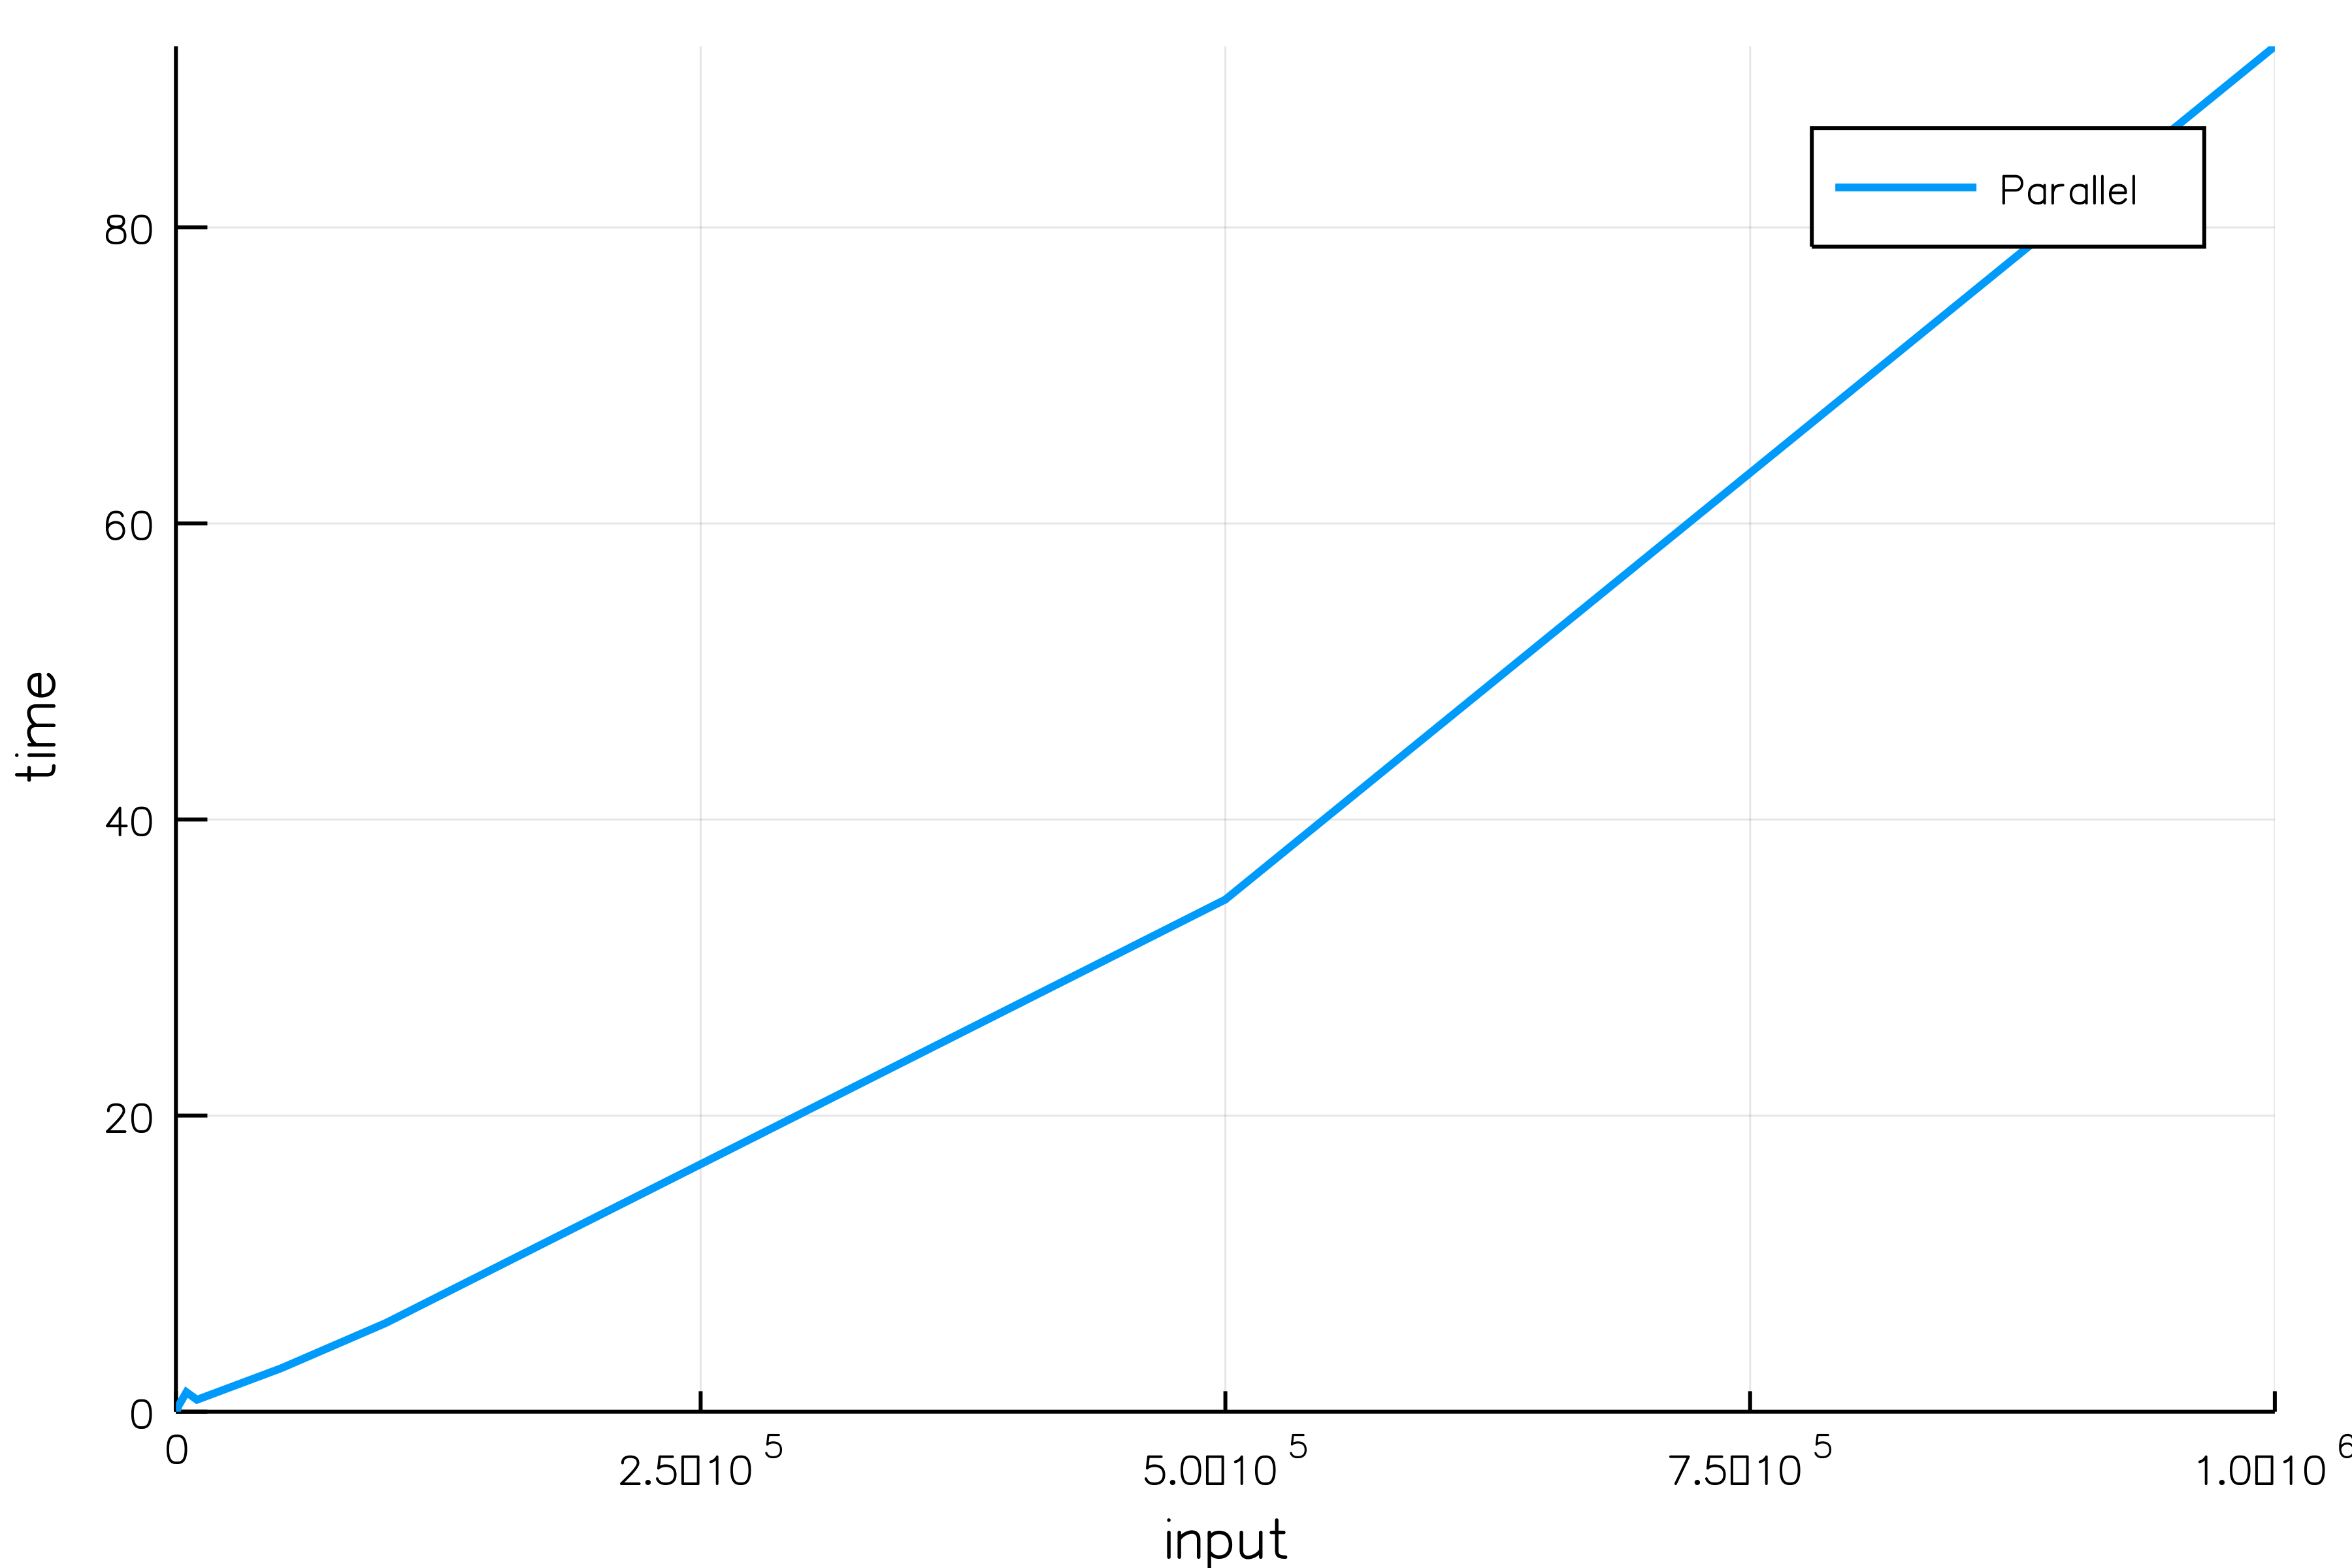
\includegraphics[width=11cm,scale=0.3]{pembedstruct.png}
\end{figure}
\begin{verbatim}
yc=[y,yp]
pc=plot(input,yc,label=["Serial" "Parallel"])
\end{verbatim}
\begin{figure}[ht!]
\centering
\includegraphics[width=11cm,scale=0.5]{compembedstruct.png}
\end{figure}
\newpage
\subsection{removeDups}
\subsubsection{Conversion}
\textbf{Python}
\begin{lstlisting}[language=Julia,format=Julia]
def removeDups (CW):{
    CW = list(set(AA(tuple)(CW)))
    CWs = list(set(AA(tuple)  (AA(sorted)(CW))  ))
    no_duplicates = defaultdict(list)
    for f in CWs: no_duplicates[f] = [ ]
    for f in CW:{
        no_duplicates[tuple(sorted(f))] += [f]}
    CW = [f[0] for f in no_duplicates.values()]
    return CW
\end{lstlisting}
\textbf{Julia}
\begin{lstlisting}[language=Julia,format=Julia]
function removeDups(CW){
	CW=collect(Set(CW))
	CWs=collect(map(sort,CW))
	no_duplicates=Dict()
	for f in CWs{
		no_duplicates[f] = [ ]}
	end	
	for f in CW{
		no_duplicates[sort(f)]=[f]}
	end	
	CW=[f[1] for f in values(no_duplicates)]
	return CW}
end 
\end{lstlisting}
\subsubsection{Parallelization}
\begin{lstlisting}[language=Julia,format=Julia]
function premoveDups(CW){
	CW=collect(Set(CW))
	CWs=collect(@sync pmap(sort,CW))
	no_duplicates=Dict()
	@parallel for f in CWs{
		no_duplicates[f] = [ ]}
	end
	@parallel for f in CW{
		no_duplicates[sort(f)]=[f]}
	end
	 @parallel for f in values(no_duplicates){
			append!(CW,f[1])}
		end}
	return CW}
end
\end{lstlisting}
\subsubsection{Unit-Test}
\begin{lstlisting}[language=Julia]
CW1=[[0,1,2,3],[4,5,6,7],[0,1,4,5],[2,3,6,7],[0,2,4,6],[1,3,5,7],
     [4,5,6,7],[8,9,10,11],[4,5,8,9],[6,7,10,11],[4,6,8,10],[5,7,9,11]]
CW2=[[0,1,2,3],[4,5,6,7],[8,9,10,11],[12,13,14,15],[16,17,18,19]]

@testset "removeDups Tests" begin
   @testset "removeDups 3D" begin
      @test length(removeDups(CW1))<= length(CW1)
      @test typeof(removeDups(CW1))==Array{Array{Int64,1},1}
   end
   @testset "removeDups 2D" begin
      @test length(removeDups(CW2))<= length(CW2)
      @test typeof(removeDups(CW2))==Array{Array{Int64,1},1}
   end
end

CW1=[[0,1,2,3],[4,5,6,7],[0,1,4,5],[2,3,6,7],[0,2,4,6],[1,3,5,7],
     [4,5,6,7],[8,9,10,11],[4,5,8,9],[6,7,10,11],[4,6,8,10],[5,7,9,11]]
CW2=[[0,1,2,3],[4,5,6,7],[8,9,10,11],[12,13,14,15],[16,17,18,19]]

@testset "premoveDups Tests" begin
   @testset "premoveDups 3D" begin
      @test length(premoveDups(CW1))<= length(CW1)
      @test typeof(premoveDups(CW1))==Array{Array{Int64,1},1}
   end
   @testset "premoveDups 2D" begin
      @test length(premoveDups(CW2))<= length(CW2)
      @test typeof(premoveDups(CW2))==Array{Array{Int64,1},1}
    end
end
\end{lstlisting}
\newpage
\subsection{struct2lar}
\subsubsection{Conversion}
\textbf{Python}
\begin{lstlisting}[language=Python,format=Julia]
def prepKey (args): return "["+", ".join(args)+"]"

def fixedPrec(PRECISION):{
    def fixedPrec0(value):{
        out = round(value*10**(PRECISION))/10**(PRECISION)
        if out == -0.0: out = 0.0
        return str(out)}
    return fixedPrec0}
    
def vcode (PRECISION=4):{
    def vcode0 (vect):{
        return prepKey(AA(fixedPrec(PRECISION))(vect))}
    return vcode0
\end{lstlisting}
This is not the original function of the larlib module. The original function did not run and this is the modified function that runs:
\begin{lstlisting}[language=Python,format=Julia]
def struct2lar(structure,metric=ID):{
    listOfModels = evalStruct(structure)
    vertDict = dict()
    index,defaultValue,CW,W,FW = -1,-1,[ ],[ ],[ ]        
    for model in listOfModels:{
    	if isinstance(model,Model):{
            V= model.verts
            FV=model.cells}                        
        elif (isinstance(model,tuple) or isinstance(model,list)):{
            if len(model)==2: {
                print(len(model))
                V,FV=model
                dim=len(model)}				
            elif len(model)==3: {
				V,FV,EV,dim=model,len(model)
				for k,incell in enumerate(EV):{
					outcell = [ ]
					for v in incell:{
						key = vcode(4)(A[v])
						if vertDict.get(key,defaultValue) == defaultValue:{
							index += 1
							vertDict[key] = index
							outcell += [index]
							W += [eval(key)]}
						else: {
							outcell += [vertDict[key]]}}
					FW += [outcell]}
        for k,incell in enumerate(FV):{
            outcell = []
            for v in incell:{
                key = vcode(4)(V[v])
                if vertDict.get(key,defaultValue) == defaultValue:{
                    index += 1
                    vertDict[key] = index
                    outcell += [index]
                    W += [eval(key)]}
                else: {
                    outcell += [vertDict[key]]}
            CW += [outcell]}}      
    if ((isinstance(model,tuple) or isinstance(model,list)) {?and len(model)==2) or ((isinstance(model,Model){? and model.n==2)): }}}
        if len(CW[0])==2: {
            CW = list(set(AA(tuple)(AA(sorted)(CW))))}
        else: CW = removeDups(CW)
        return metric(W),CW}
    if ((isinstance(model,tuple) or isinstance(model,list)) {?and len(model)==3): }
        FW = list(set(AA(tuple)(AA(sorted)(FW))))
        CW = removeDups(CW)
        return metric(W),CW,FW
\end{lstlisting}
\textbf{Julia}
\begin{lstlisting}[language=Julia,format=Julia]
function fixedPrec(PRECISION){
	function fixedPrec0(value) {
		out=round.(value,PRECISION)
		if out==-0.0{
			out=0.0}
		end
		return string(out)}
	end
	return fixedPrec0}
end

function vcode(PRECISION=4){
	function vcode0(vect){
		return fixedPrec(PRECISION)(vect) }
	end
	return vcode0}
end

function struct2lar(structure){
	listOfModels=evalStruct(structure)
	vertDict= Dict()
	index,defaultValue,CW,W,FW = -1,-1,[ ],[ ],[ ]	
	for model in listOfModels{
		if  length(model)==2{
			V,FV=model}
		elseif lenght(model)==3{
			V,FV,EV=model}
		end
		for (k,incell) in enumerate(FV){
			outcell=[ ]
			for v in incell{
				key=vcode(4)(V[v+1])
				if get(vertDict,key,defaultValue)==defaultValue{
					index =index+1
                   			vertDict[key]=index
					append!(outcell,index)
					append!(W,[eval(parse(key))])      }             
				else{
					append!(outcell,vertDict[key])}
				end}
			end
			append!(CW,[outcell])}
		end
		if length(model)==3{
			for (k,incell) in enumerate(FV){
				outcell=[ ]
				for v in incell{
					key=vcode(4)(V[v+1])
					if get(vertDict,key,defaultValue)==defaultValue{
						index =index+1
						vertDict[key]=index
						append!(outcell,[index])
						append!(W,[eval(parse(key))]) }                 
					else{
						append!(outcell,vertDict[key])}
					end}
				end
				append!(FW,[outcell])}
			end}
		end}
	end	
	if length(listOfModels[end])==2{
		if length(CW[1])==2{
			CW=map(Tuple,map(sort,CW))}
		else{
			CW=removeDups(CW)}
		end
		return W,CW}
	end	
	if length(listOfModels[end])==3{
		FW=map(Tuple,map(sort,FW))
		CW=removeDups(CW)
		return W,CW,FW}
	end}
end
\end{lstlisting}
\subsubsection{Parallelization}
\begin{lstlisting}[language=Julia,format=Julia]
@everywhere function pfixedPrec(PRECISION){
	function pfixedPrec0(value) {
		out=round.(value,PRECISION)
		if out==-0.0{
			out=0.0}
		end
		return string(out)}
	end
	return pfixedPrec0}
end

function pvcode(PRECISION=4){
	function pvcode0(vect){
		return pfixedPrec(PRECISION)(vect) }
	end
	return pvcode0}
end

@everywhere function pstruct2lar(structure){
	listOfModels=pevalStruct(structure)
	vertDict= Dict()
	index,defaultValue,CW,W,FW = -1,-1,[ ],[ ],[ ]	
	for model in listOfModels{
		if  length(model)==2{
			V,FV=model}
		elseif lenght(model)==3{
			V,FV,EV=model}
		end
		@sync begin{
			for (k,incell) in enumerate(FV){
				outcell=[ ]
			@async begin{
			      for v in incell{
			      	  key=pvcode(4)(V[v+1])
				  if get(vertDict,key,defaultValue)==defaultValue{
					index =index+1
                    			vertDict[key]=index
					append!(outcell,index)
					append!(W,[eval(parse(key))])}
				  else{
					append!(outcell,vertDict[key])}
				  end}
			       end	}
			end
			append!(CW,[outcell])}
			end}
		end
		if length(model)==3{
		   	@sync begin{
				for (k,incell) in enumerate(FV){
					outcell=[ ]
					@async begin{
				       	       for v in incell{
				       	       	   key=pvcode(4)(V[v+1])
							if get(vertDict,key,defaultValue)==defaultValue{
							   index =index+1
							   vertDict[key]=index
							   append!(outcell,[index])
							   append!(W,[eval(parse(key))])    }               
					   		else{
								append!(outcell,vertDict[key])}
							end}
						end}
					end
				append!(FW,[outcell])}
				end}
			end}
		end}
	end	
	if length(listOfModels[end])==2{
		if length(CW[1])==2{
			CW=pmap(Tuple,pmap(sort,CW))}
		else{
			CW=premoveDups(CW)}
		end
		return W,CW}
	end	
	if length(listOfModels[end])==3{
		FW=pmap(Tuple,pmap(sort,FW)) 
		CW=premoveDups(CW)
		return W,CW,FW}
	end}
end
\end{lstlisting}
\subsubsection{Unit-Test}
\begin{lstlisting}[language=Julia]
@testset "struct2lar" begin
   @testset "struct2lar 2D" begin
      square=([[0, 0],[0,1],[1,0],[1,1]],[[0,1,2,3]])
      table=larApply(t(-0.5,-0.5))(square)
      structure=Struct([repeat([table,r(pi/2)],outer=2)...])
      @test typeof(struct2lar(structure))==Tuple{Array{Any,1},
      Array{Array{Any,1},1}}
      @test length(struct2lar(structure)[1][1])==2
   end
   @testset "struct2lar 3D" begin
       BV=[[0,1,2,3],[4,5,6,7],[0,1,4,5],[2,3,6,7],[0,2,4,6],[1,3,5,7]]
      V=[[0 0,0],[0,0,1],[0,1,0],[0,1,1],[1,0,0],
         [1,0,1],[1,1,0],[1,1,1]]
      block=[V,BV]
      structure=Struct(repeat([block,t(1,0,0)],outer=2));
      @test typeof(struct2lar(structure))==Tuple{Array{Any,1},
      Array{Array{Any,1},1}}
      @test length(struct2lar(structure)[1][1])==3
    end
end

@testset "pstruct2lar" begin
   @testset "pstruct2lar 2D" begin
      square=([[0, 0], [0, 1], [1, 0], [1, 1]], [[0, 1, 2, 3]])
      table=plarApply(t(-0.5,-0.5))(square)
      structure=pStruct([repeat([table,r(pi/2)],outer=2)...])
      @test typeof(pstruct2lar(structure))==Tuple{Array{Any,1},Array{Any,1}}
      @test length(pstruct2lar(structure)[1][1])==2
   end
   @testset "pstruct2lar 3D" begin
       BV=[[0,1,2,3],[4,5,6,7],[0,1,4,5],[2,3,6,7],[0,2,4,6],[1,3,5,7]]
      V=[[0 0,0],[0,0,1],[0,1,0],[0,1,1],[1,0,0],
         [1,0,1],[1,1,0],[1,1,1]]
      block=[V,BV]
      structure=pStruct(repeat([block,t(1,0,0)],outer=2));
      @test typeof(pstruct2lar(structure))==Tuple{Array{Any,1},Array{Any,1}}
      @test length(pstruct2lar(structure)[1][1])==3
   end
end
\end{lstlisting}
\subsubsection{Results}
\textbf{Tesla}
\begin{lstlisting}[language=Julia]
input=[1,10,50,10^2,5*10^2,10^3,5*10^3,10^4,5*10^4,10^5,5*10^5,10^6]
function timeFstruct(f::Function,pf::Function,model,input)
   t=Array{Float64}(length(input))
   pt=Array{Float64}(length(input))
   for i in range(1,length(input))
      structo=addn2D(input[i],model)
      pstructo=pStruct(structo.body)
      f(structo)
      pf(pstructo)
      t[i]=@elapsed f(structo)
      pt[i]=@elapsed pf(pstructo)
   end
   return t,pt
end
\end{lstlisting}
\newpage
\begin{verbatim}
y,yp=timeFstruct(struct2lar,pstruct2lar,square,input)
p=plot(input,y,xaxis=''input'',yaxis=''time'',xlims=(0,length(input)+1),
     ylims=(0,maximum(y)+0.5), label=[''Serial''],lw=2)
\end{verbatim}
\begin{figure}[ht!]
\centering
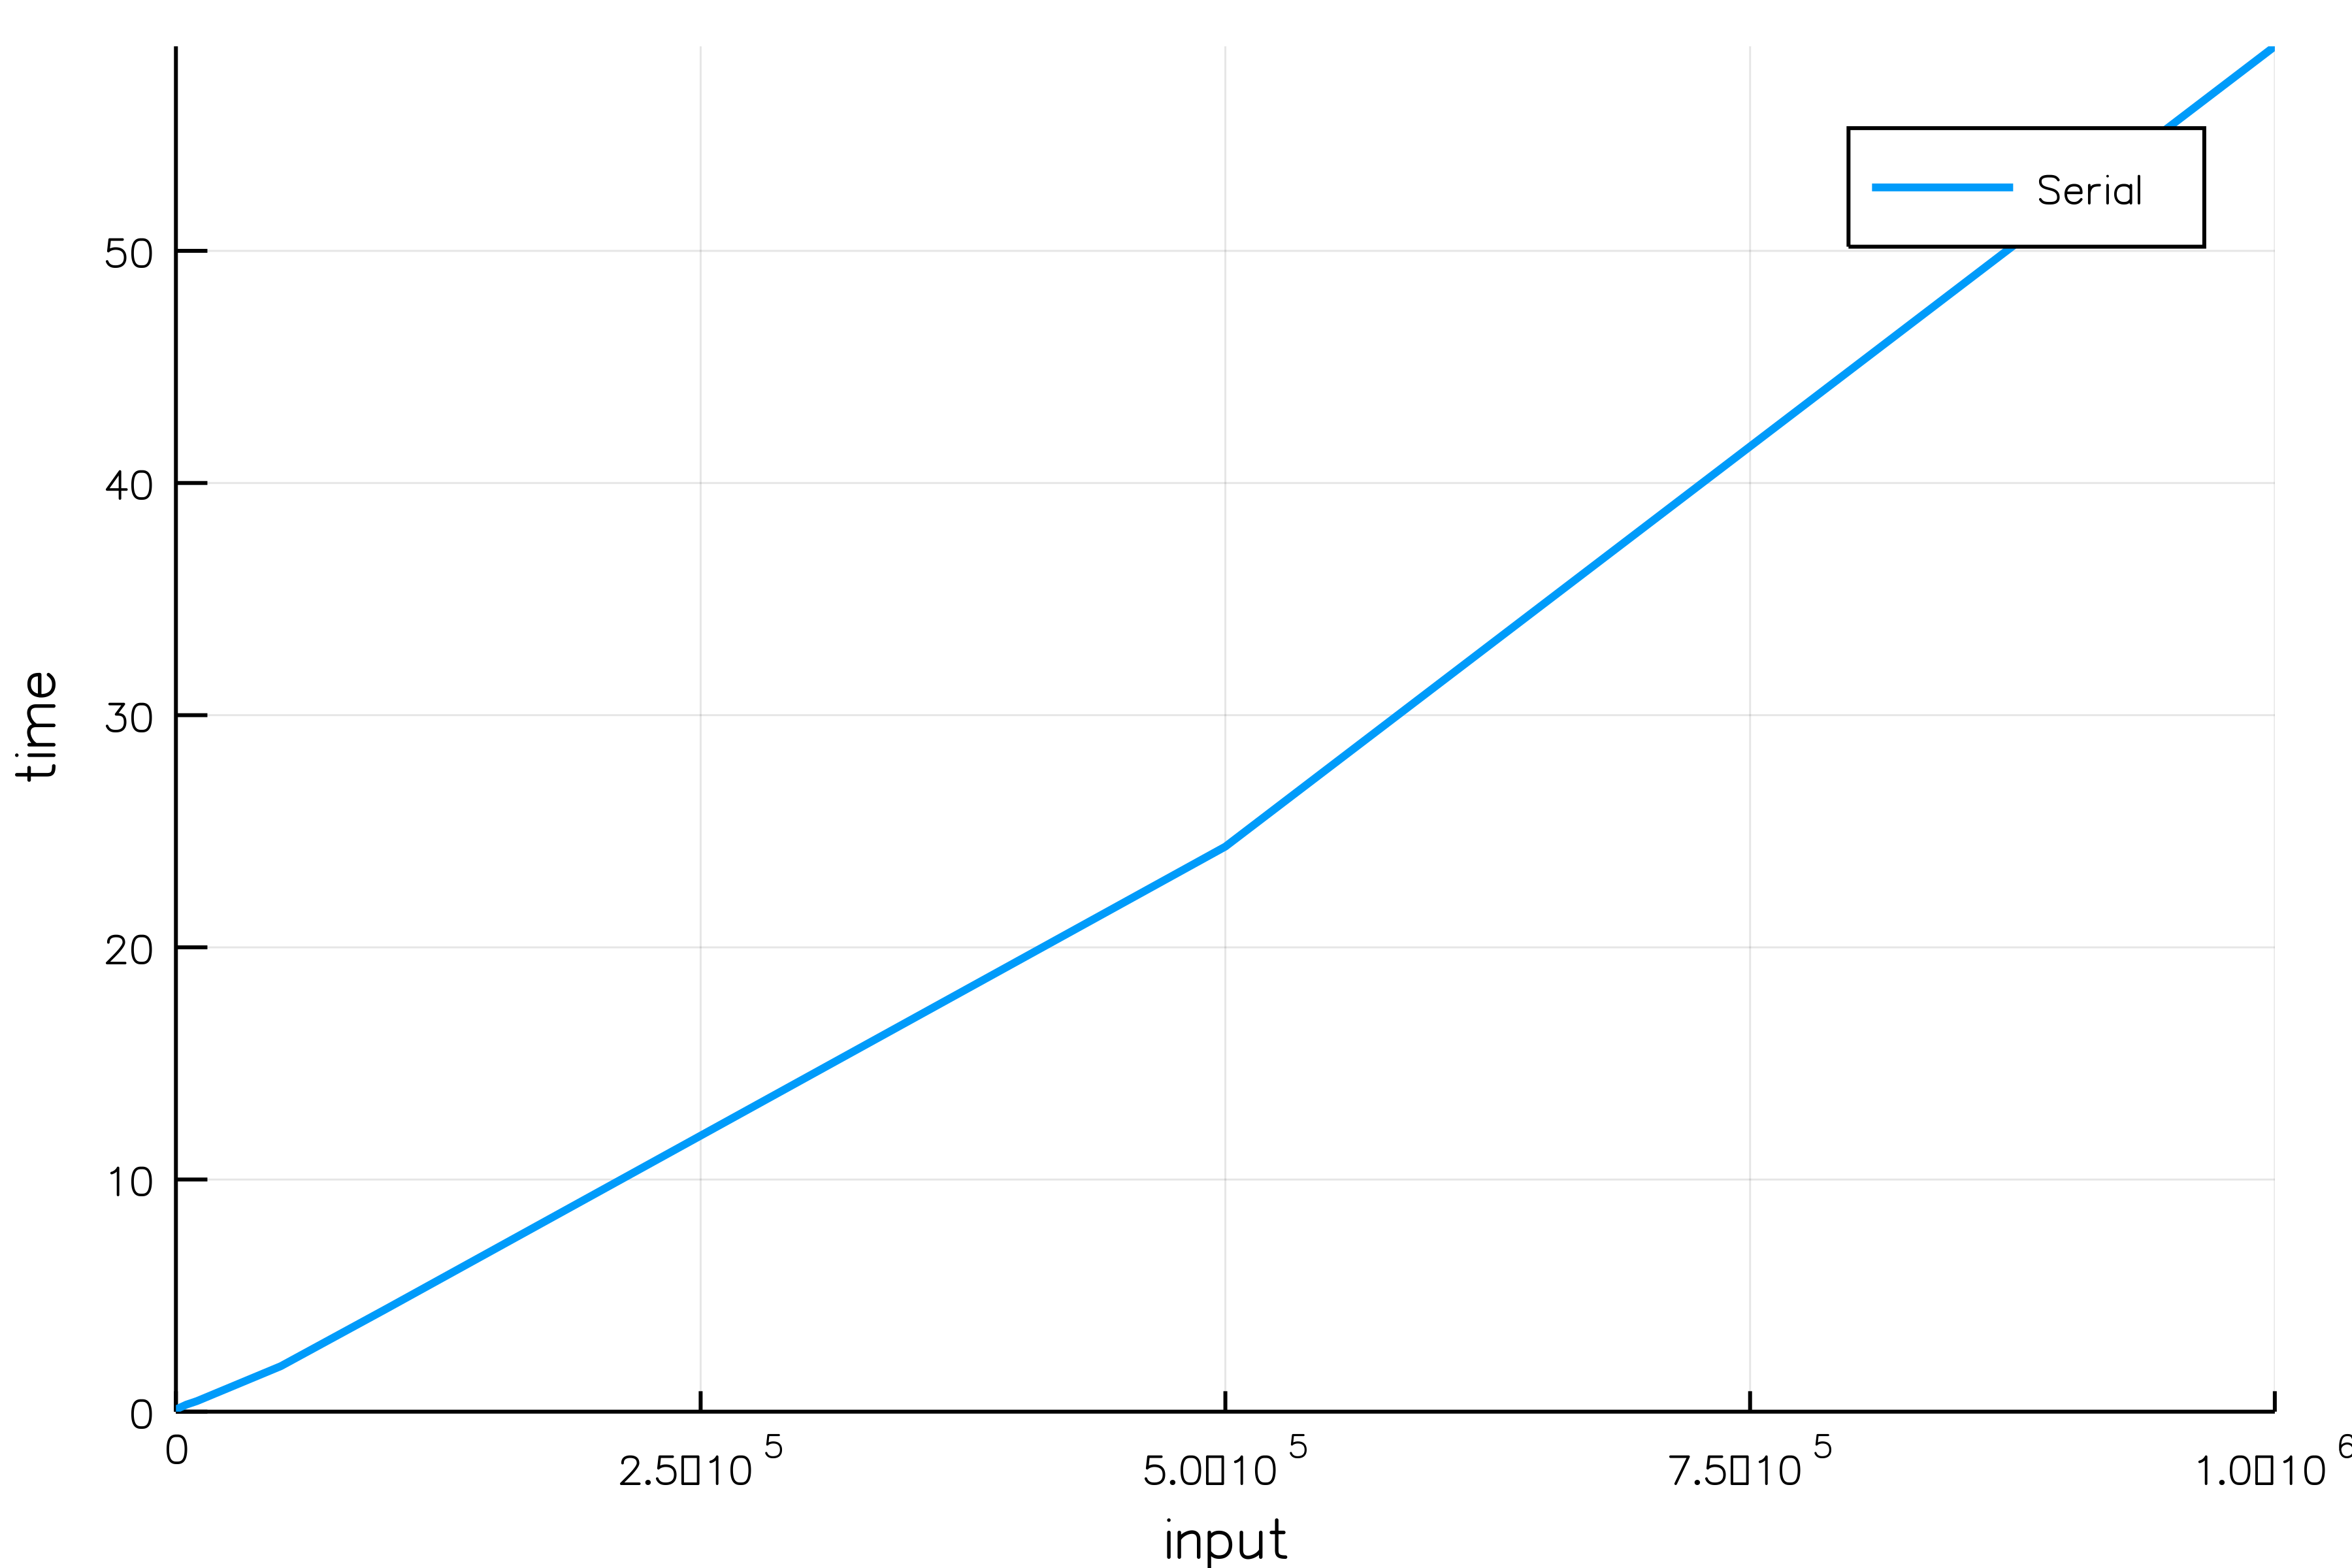
\includegraphics[width=11cm,scale=0.3]{struct2lar.png}
\end{figure}
\begin{verbatim}
pp=plot(input,yp,xaxis=''input'',yaxis=''time'',xlims=(0,length(input)+1),
       ylims=(0,maximum(y)+0.5),label=[''Parallel''],lw=2)
\end{verbatim}
\begin{figure}[ht!]
\centering
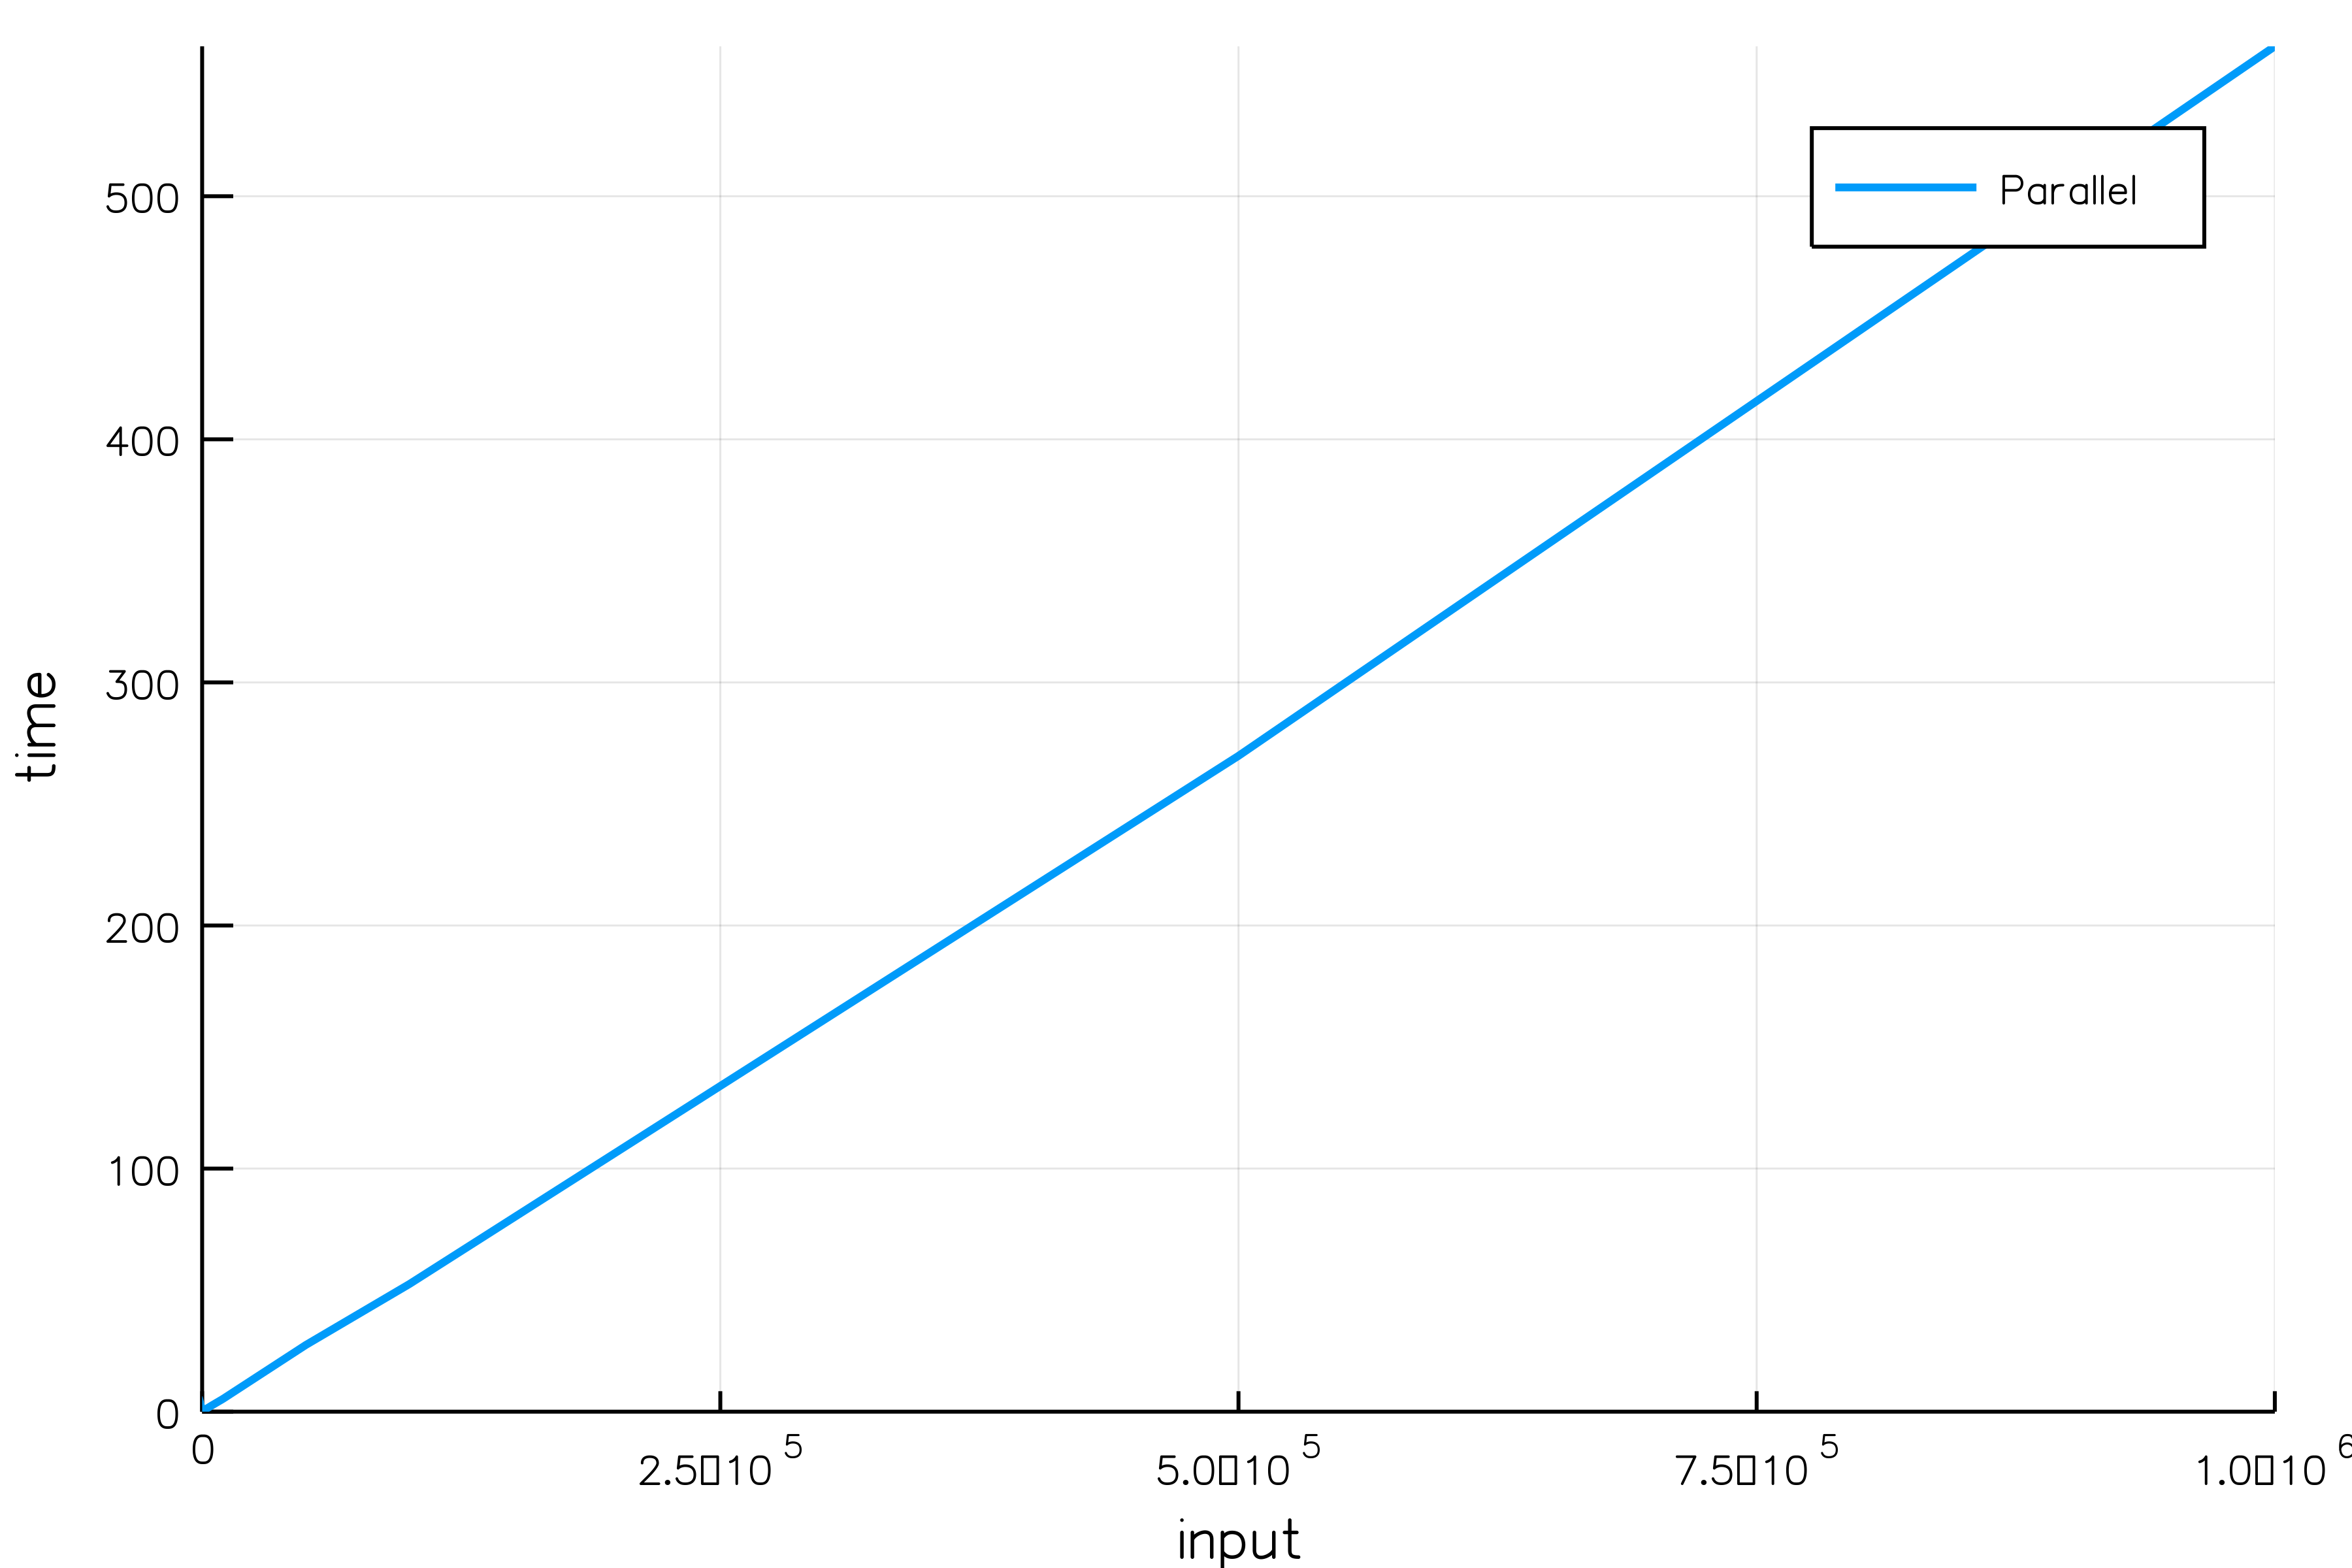
\includegraphics[width=11cm,scale=0.3]{pstruct2lar.png}
\end{figure}
\newpage
\begin{verbatim}
yc=[y,yp]
pc=plot(input,yc,label=["Serial" "Parallel"])
\end{verbatim}
\begin{figure}[ht!]
\centering
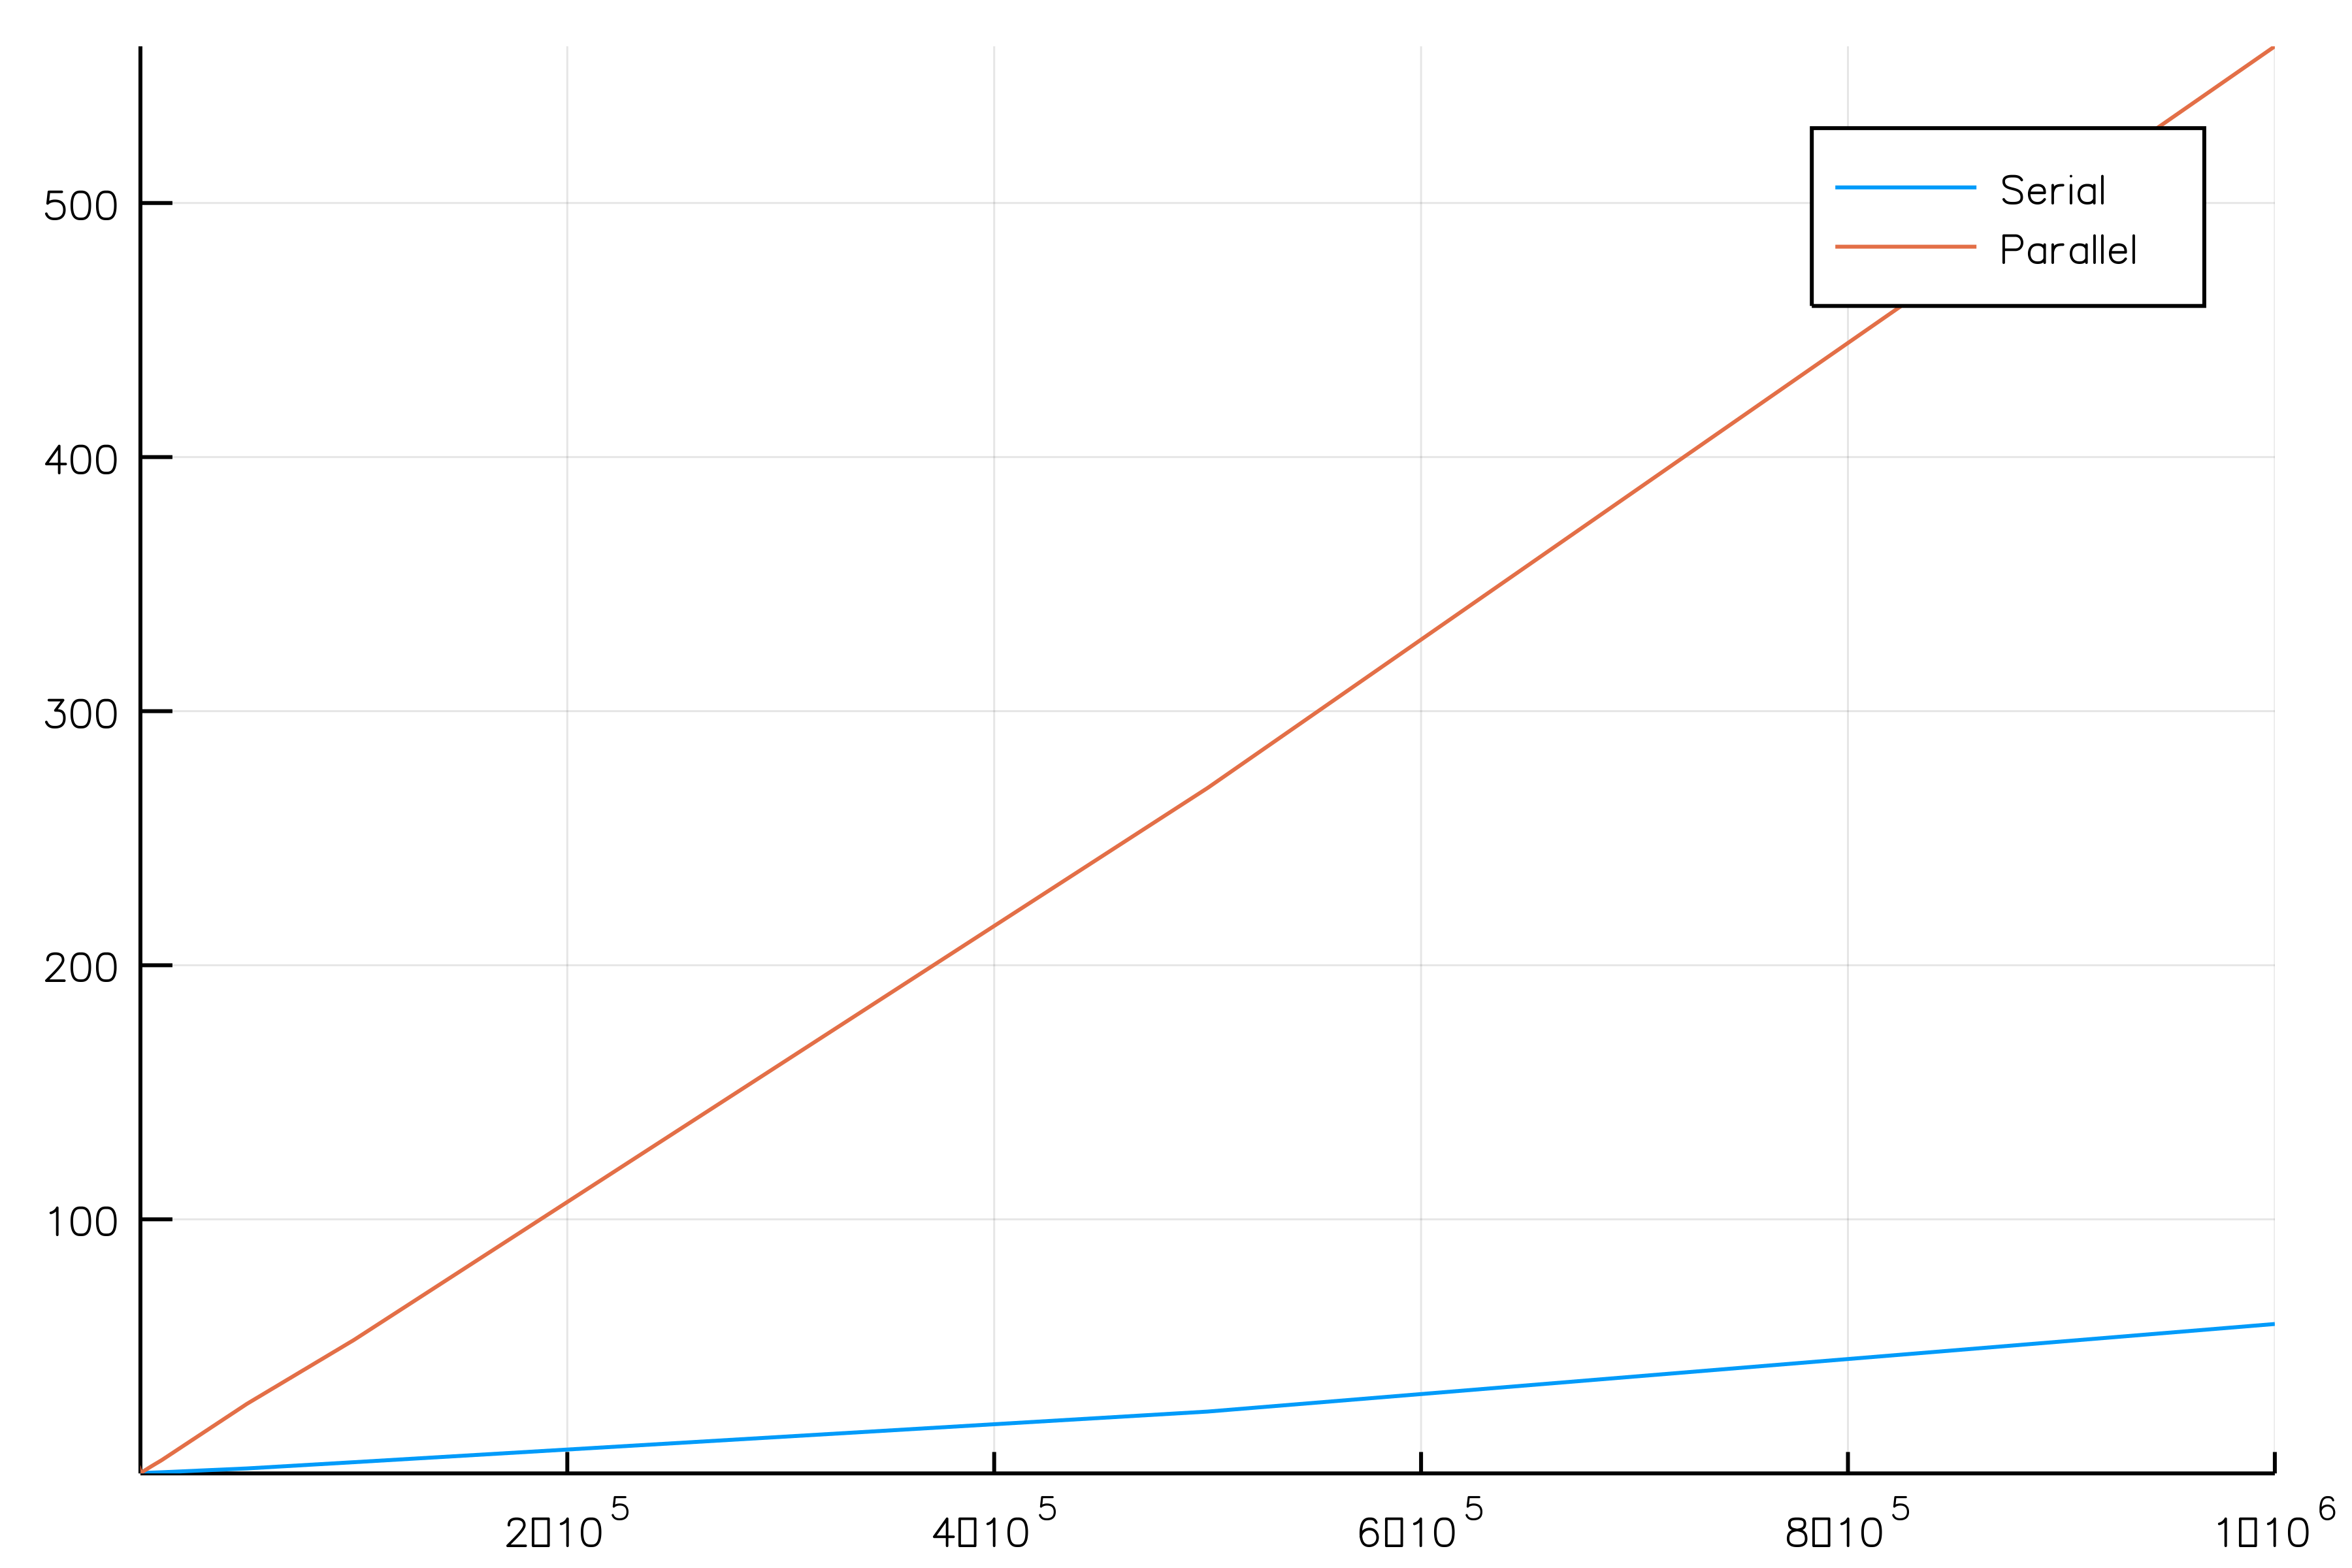
\includegraphics[width=11cm,scale=0.5]{compstruct2lar.png}
\end{figure}
\textbf{PC}
\begin{lstlisting}[language=Julia,format=Julia]
times=[ ]
ptimes=[ ]
input=[ ]
for i in range(1,length(l)-1){
    push!(input,Struct([repeat([l[i]],outer=i)...]))}
end
for i in range(1,length(input)){
    append!(times,Time(struct2lar,input[i]))}
end
for i in range(1,length(input)){
    append!(ptimes,Time(pstruct2lar,input[i]))}
end

plot(times,xlabel="input",xlims=(0,length(times)+2),{?ylabel="time(s)",label=["Serial"])
\end{lstlisting}
\newpage
\begin{figure}[ht!]
\centering
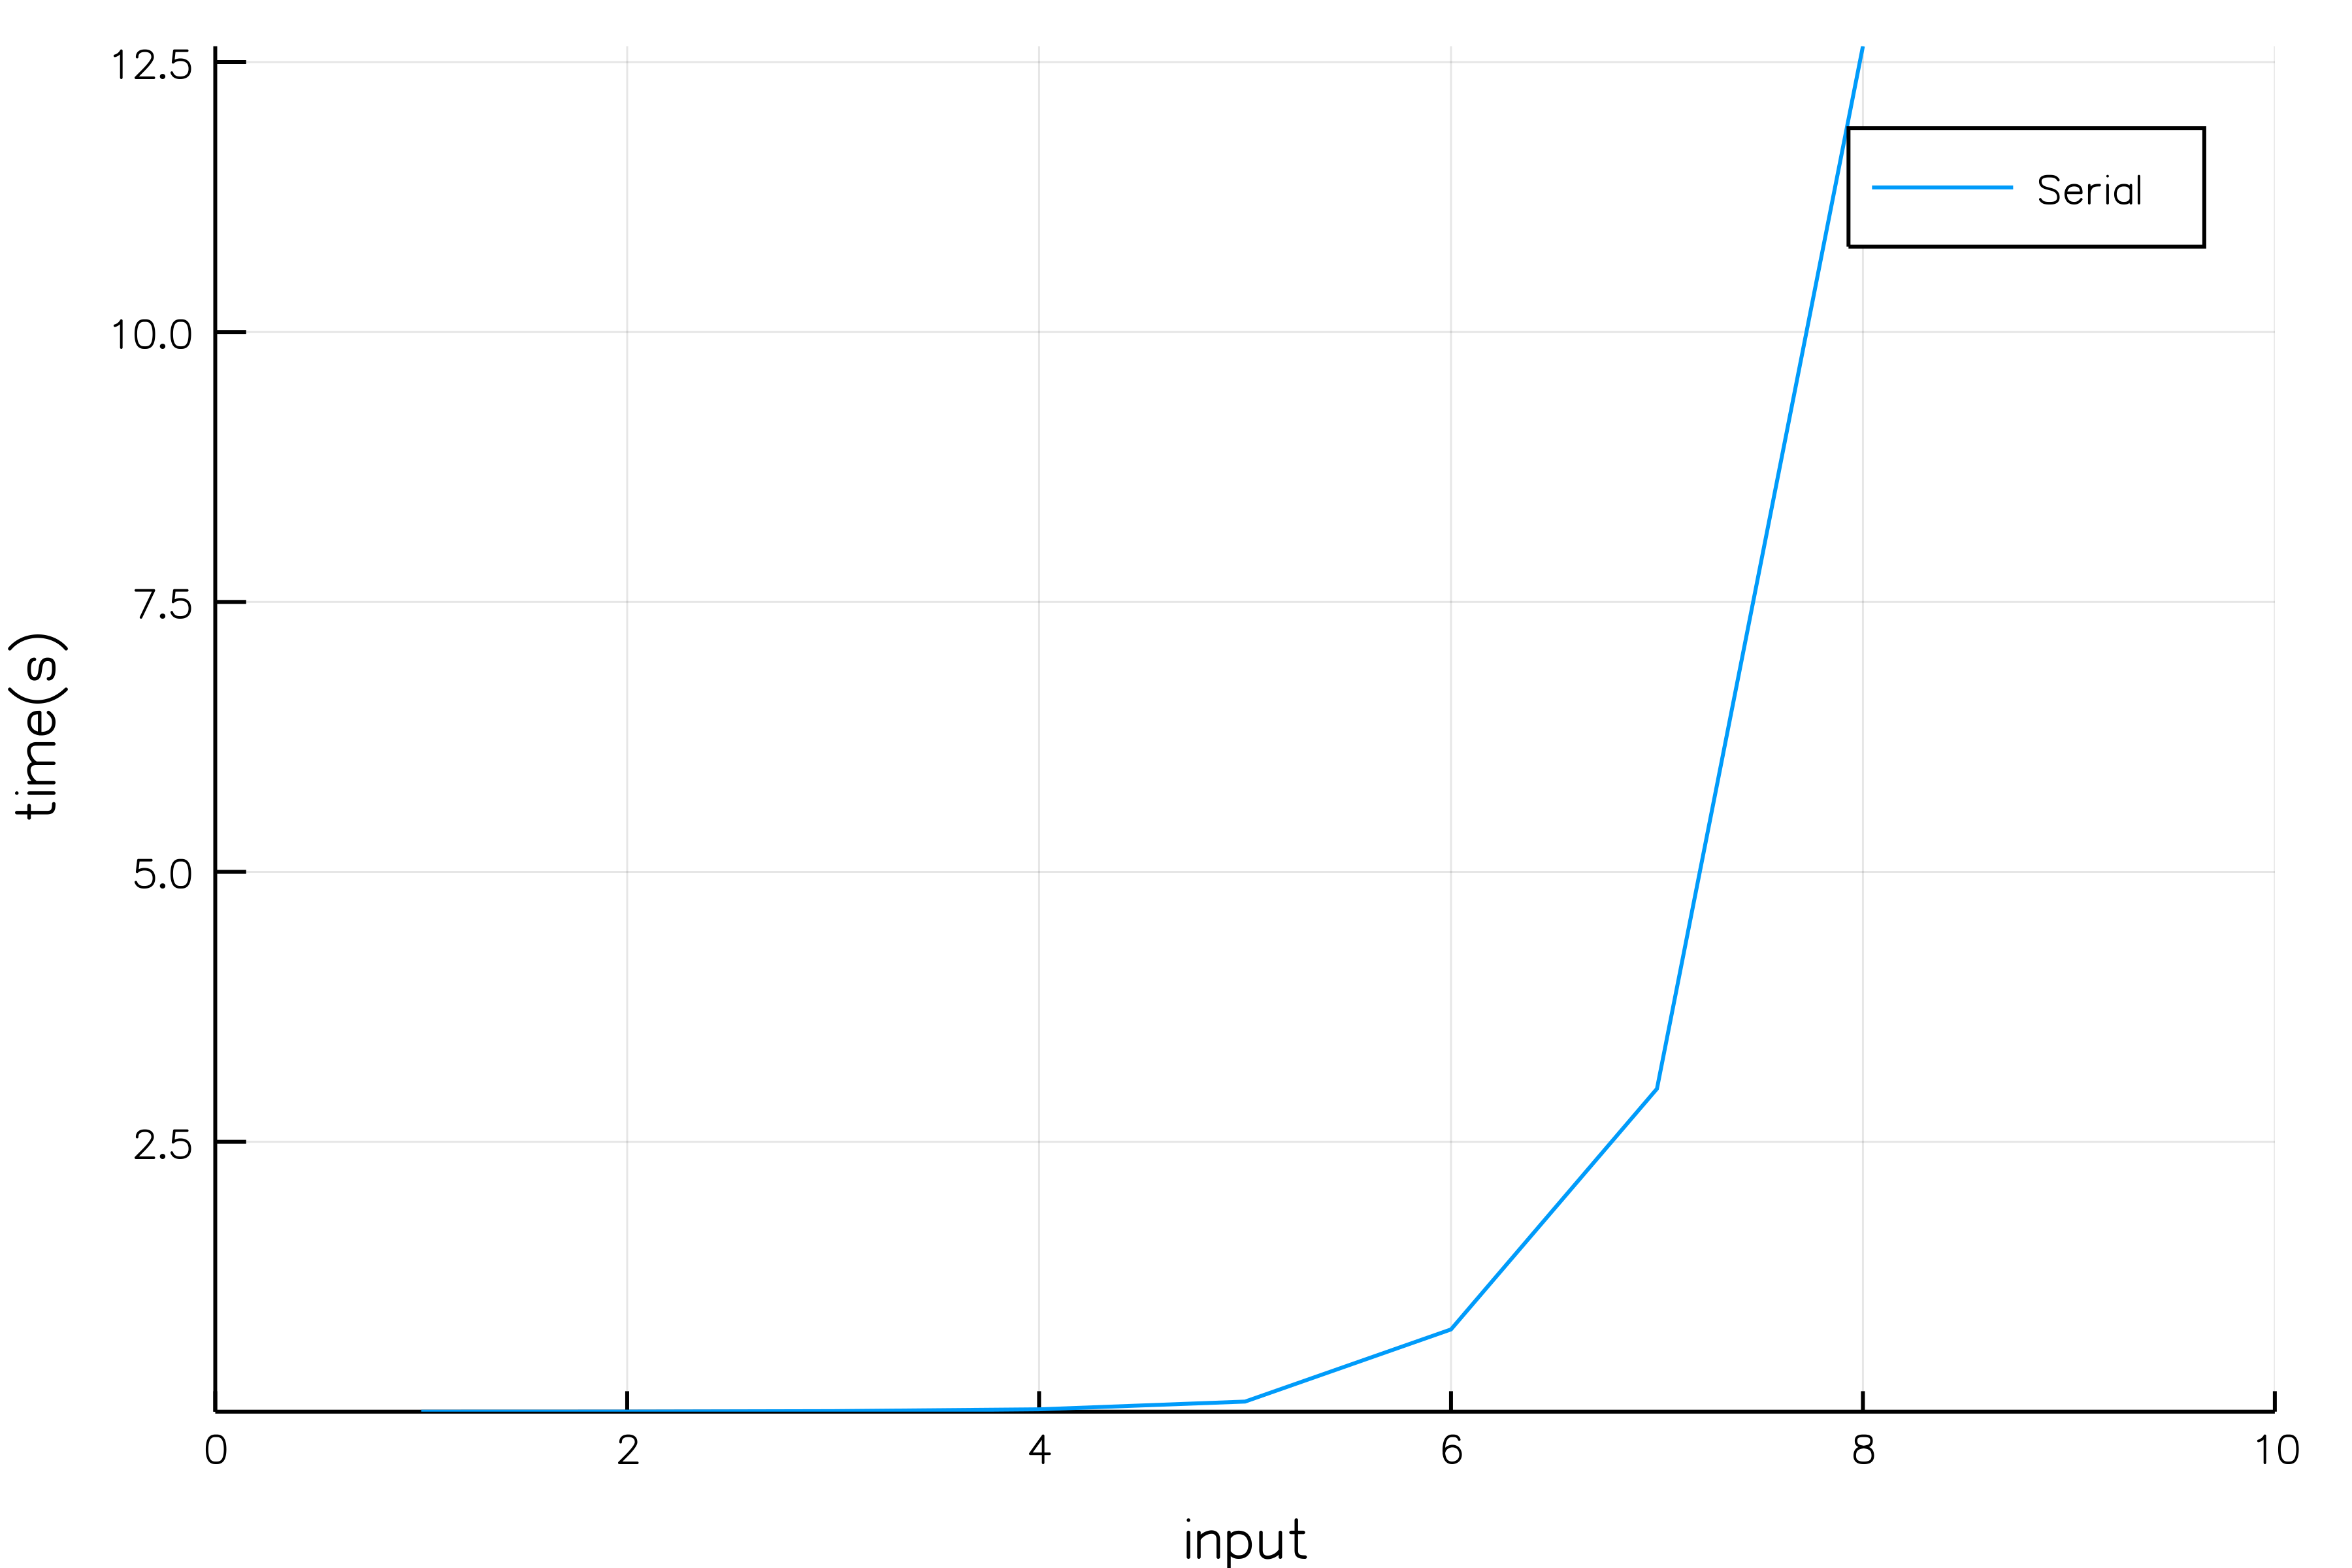
\includegraphics[width=11cm,scale=0.3]{struct2larSerial.png}
\end{figure}
\begin{lstlisting}[language=Julia,format=Julia]
plot(ptimes,xlabel="input",xlims=(0,length(times)+2),{?ylabel="time(s)",label=["Parallel"])
\end{lstlisting}
\begin{figure}[ht!]
\centering
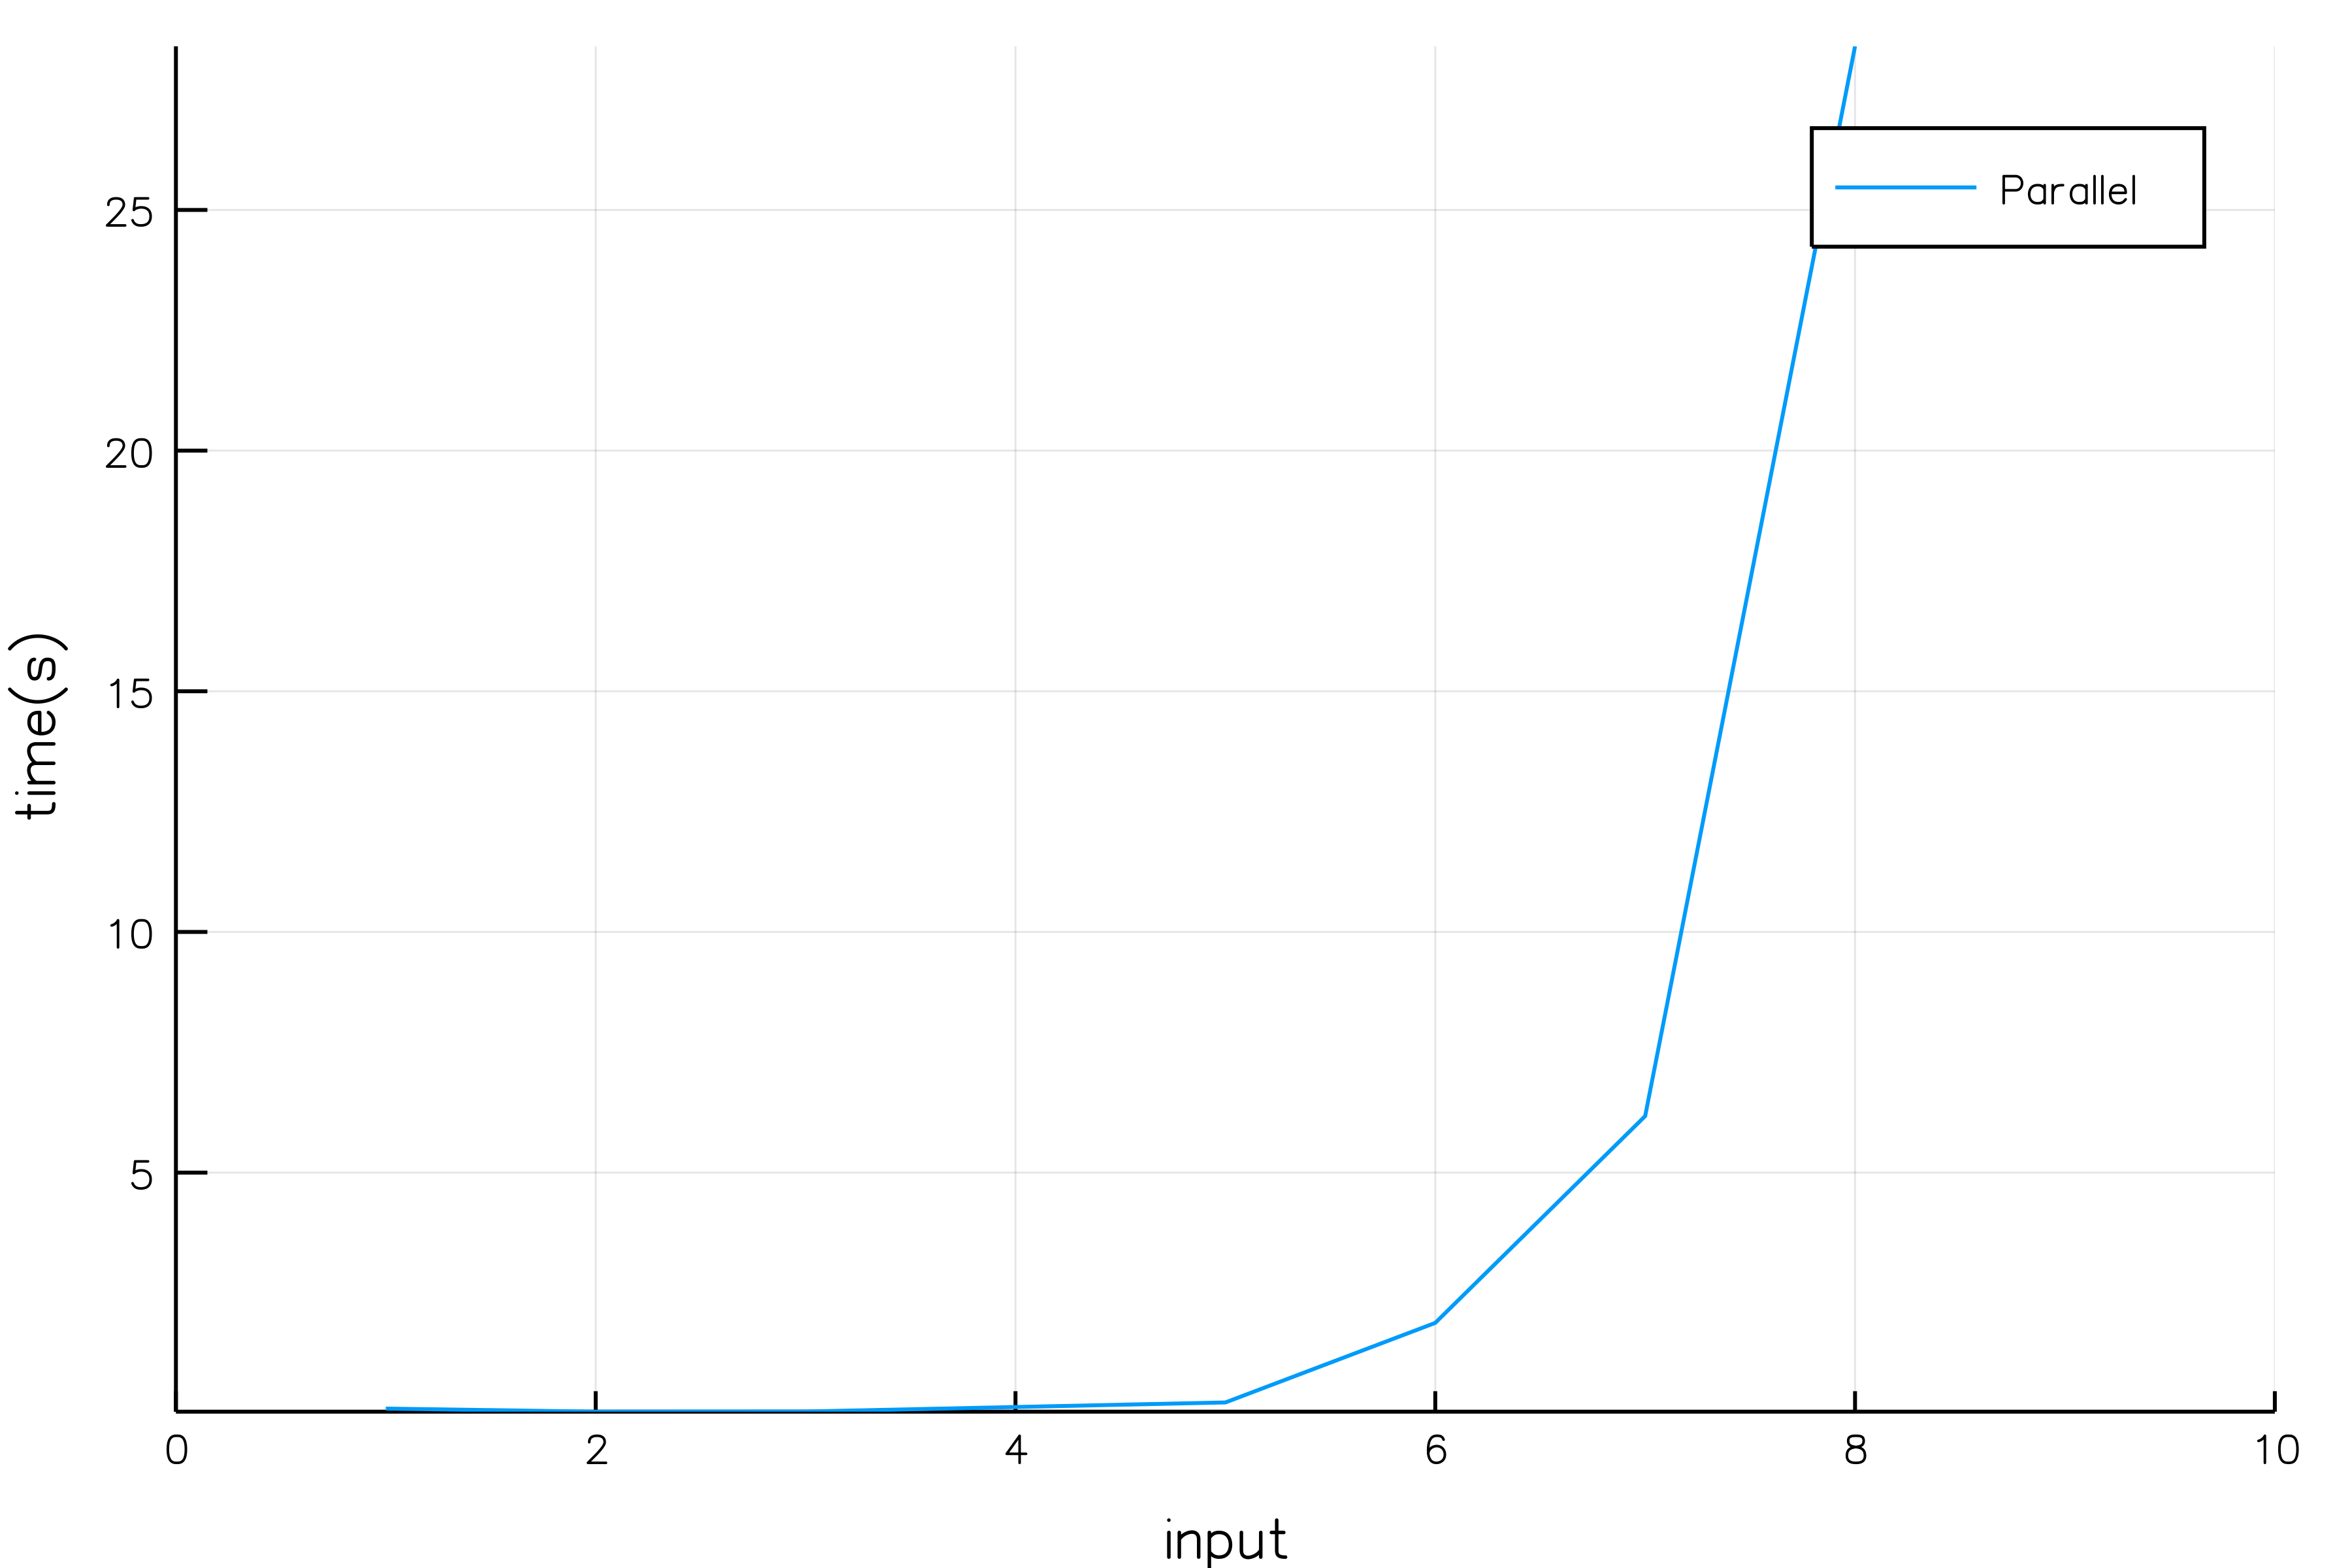
\includegraphics[width=11cm,scale=0.3]{struct2larParallel.png}
\end{figure}
\newpage
\begin{verbatim}
plot([times,ptimes],xlabel="input",xlims=(0,length(times)+2),
    ylabel="time(s)",label=["Serial","Parallel"])
\end{verbatim}
\begin{figure}[ht!]
\centering
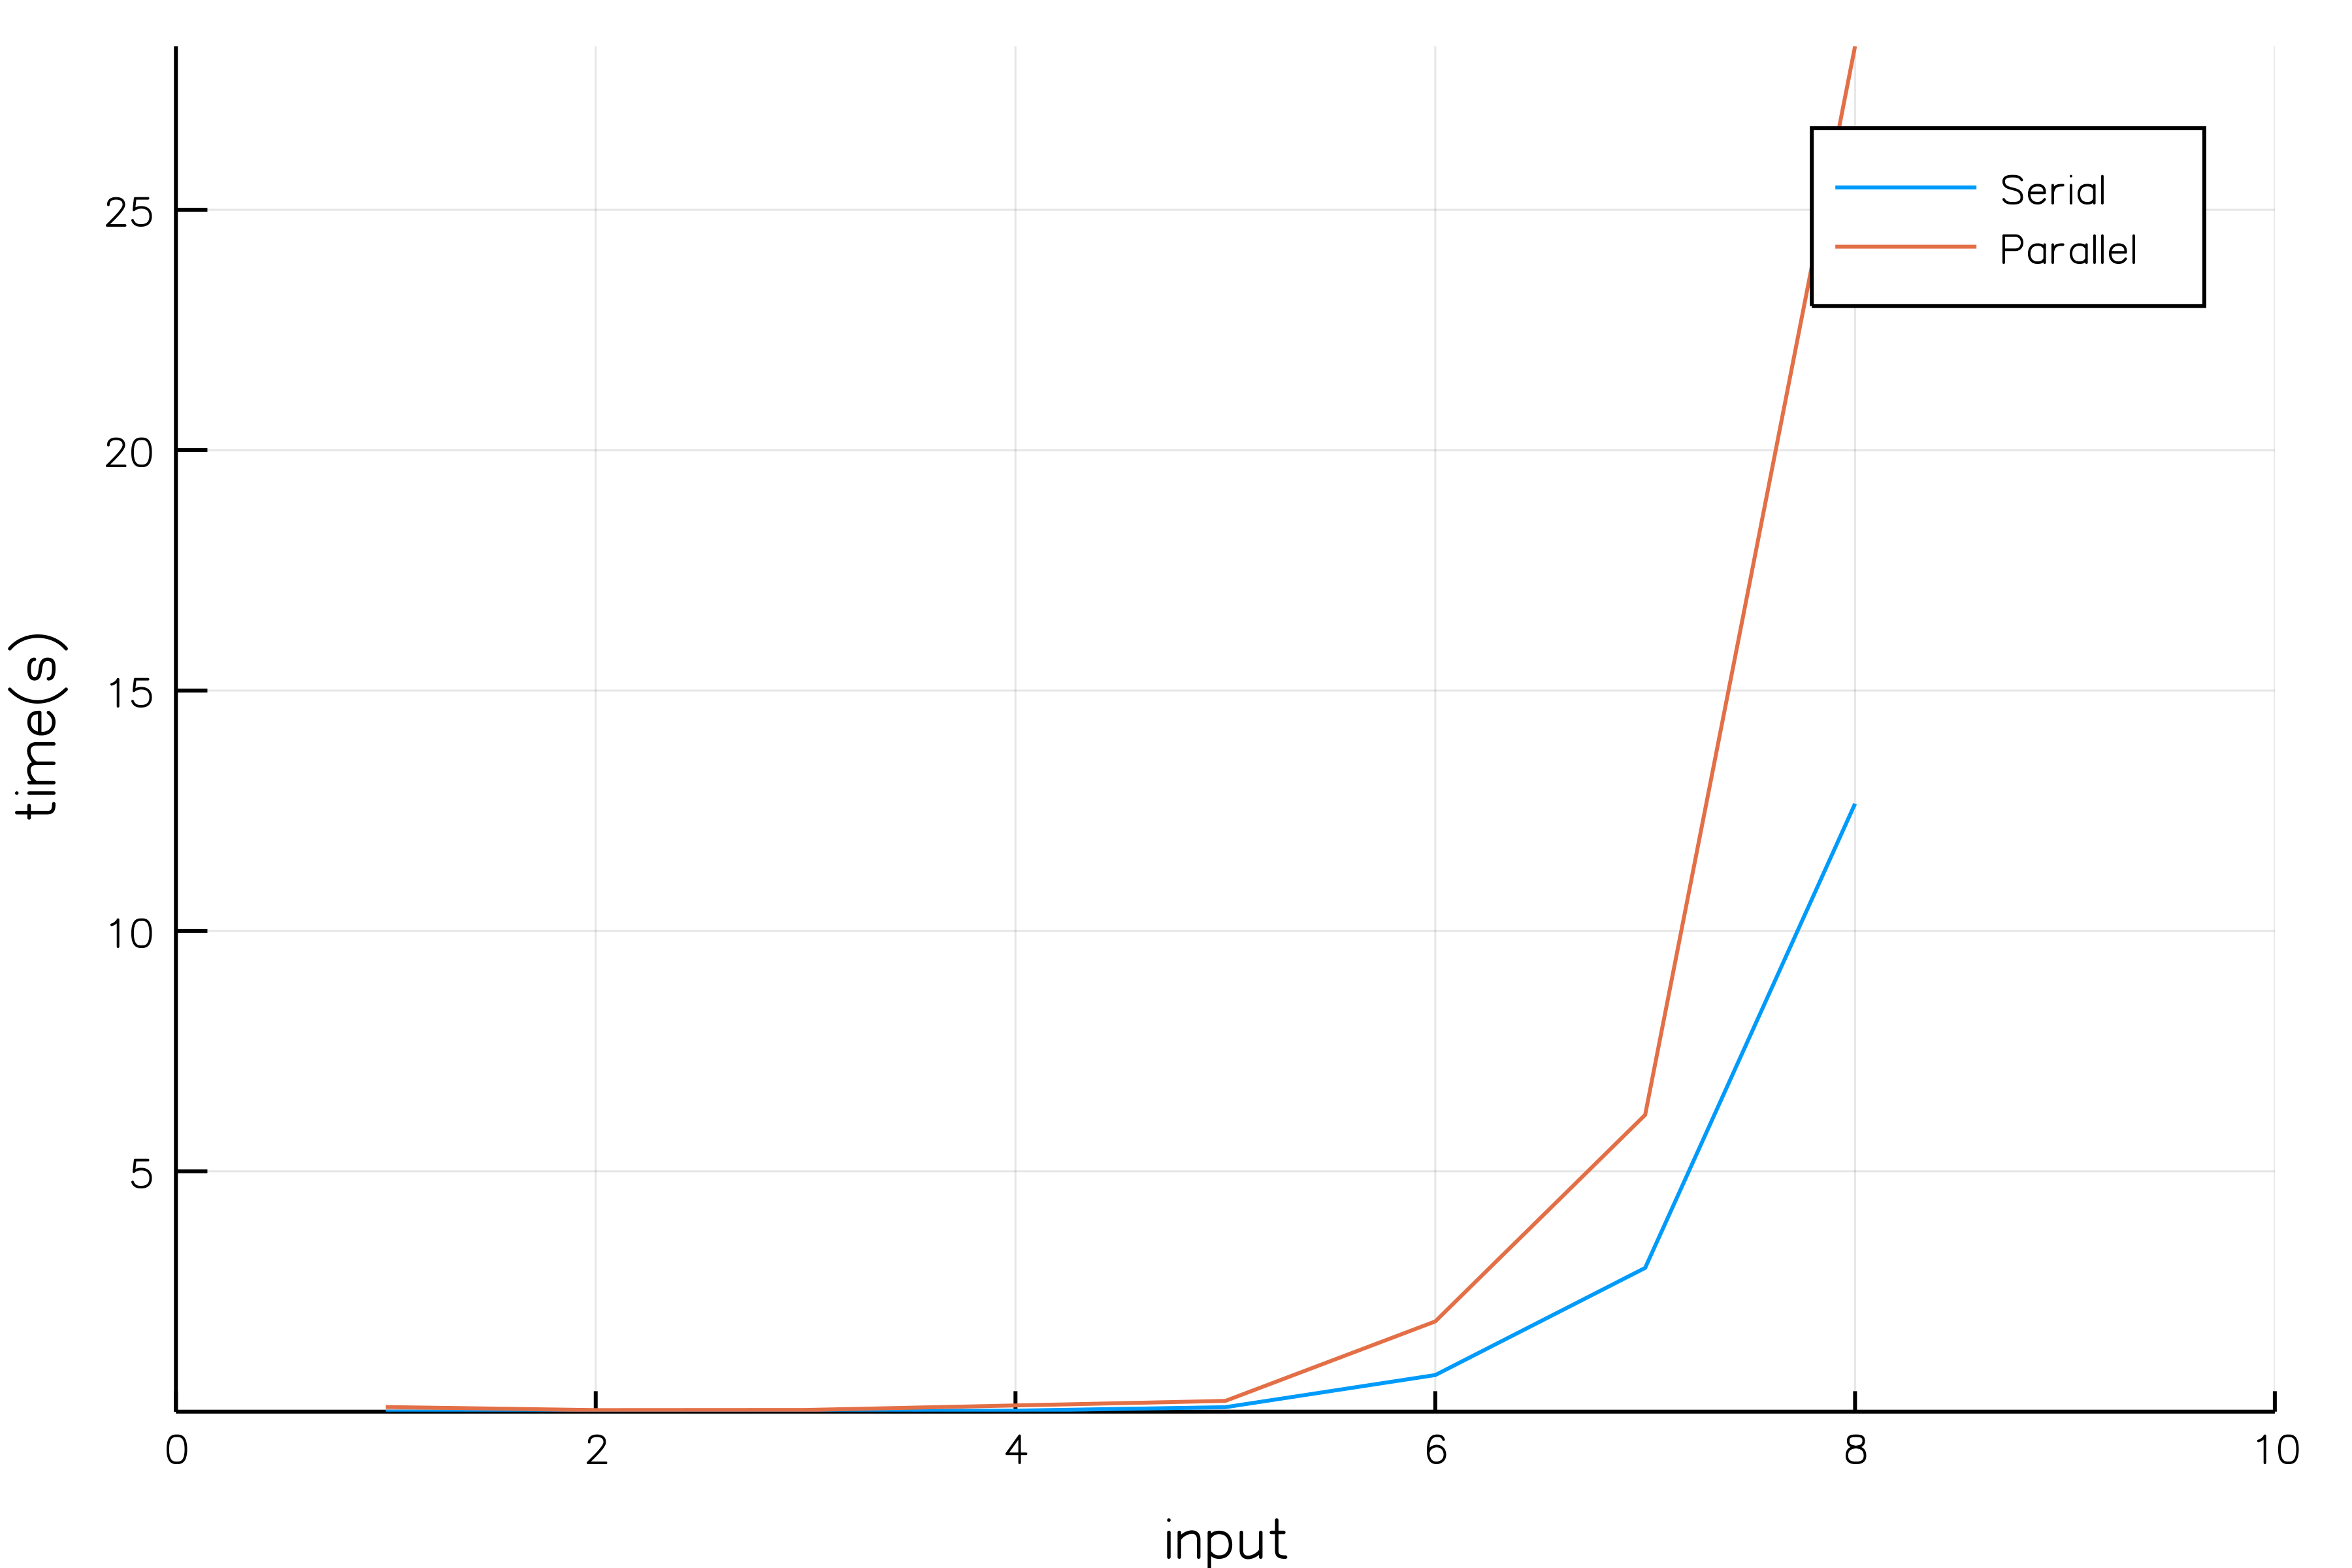
\includegraphics[width=11cm,scale=0.3]{struct2larC.png}
\end{figure}
\newpage
\subsection{larRemoveVertices}
\subsubsection{Conversion}
\textbf{Python}
\begin{lstlisting}[language=Python,format=Julia]
def larRemoveVertices(V,FV):{
    vertDict = dict()
    index,defaultValue,FW,W = -1,-1,[ ],[ ]        
    for k,incell in enumerate(FV):{
        outcell = [ ]
        for v in incell:{
            key = vcode(4)(V[v])
            if vertDict.get(key,defaultValue) == defaultValue:{
                index += 1
                vertDict[key] = index
                outcell += [index]
                W += [eval(key)]}
            else: {
                outcell += [vertDict[key]]}}
        FW += [outcell]}
    return W,FW
\end{lstlisting}
\textbf{Julia}
\begin{lstlisting}[language=Julia,format=Julia]
function larRemoveVertices(V,FV){
	vertDict= Dict()
	index,defaultValue,CW,W,FW = -1,-1,[ ],[ ],[ ]
	for (k,incell) in enumerate(FV){
		outcell=[ ]
		for v in incell{
			key=vcode(4)(V[v+1])
			if get(vertDict,key,defaultValue)==defaultValue{
				index =index+1
				vertDict[key]=index
				append!(outcell,index)
				append!(W,[eval(parse(key))])     }              
			else{
				append!(outcell,vertDict[key])}
			end}
		end
		append!(FW,[outcell])}
	end
	return W,FW}
end
\end{lstlisting}
\subsubsection{Parallelization}
\begin{lstlisting}[language=Julia,format=Julia]
@everywhere function plarRemoveVertices(V,FV){
	vertDict= Dict()
	index,defaultValue,CW,W,FW = -1,-1,[ ],[ ],[ ]
	@async begin{
	       for (k,incell) in enumerate(FV){
	       	   	outcell=[]
			@sync begin{
			      for v in incell{
			      	  key=pvcode(4)(V[v+1])
					if get(vertDict,key,defaultValue)==defaultValue{
				   	   index =index+1
				   	   vertDict[key]=index
				   	   append!(outcell,index)
				   	   append!(W,[eval(parse(key))])}
					else{
						append!(outcell,vertDict[key])}
					end}
				end}
			end
			append!(FW,[outcell])}
		end}
	end
	return W,FW}
end
\end{lstlisting}
\subsubsection{Unit-Test}
\begin{lstlisting}[language=Julia]
V=[[0,0,0],[0,0,1],[0,1,0],[0,1,1],[1,0,0],[1,0,1],
   [1, 1, 0], [1, 1, 1]]
FV=[[0,1,2,3],[4,5,6,7],[0,1,4,5],[2,3,6,7], 
[0,2,4,6],[1,3,5,7]]

@testset "larRemoveVertices Tests" begin
   @test typeof(larRemoveVertices(V,FV))==Tuple{Array{Any,1},Array{Any,1}}
   @test length(larRemoveVertices(V,FV)[1])<= length(V)
end

V=[[0,0,0],[0,0,1],[0,1,0],[0,1,1],[1,0,0],[1,0,1],
   [1, 1, 0], [1, 1, 1]]
FV=[[0,1,2,3],[4,5,6,7],[0,1,4,5],[2,3,6,7], 
[0,2,4,6],[1,3,5,7]]

@testset "plarRemoveVertices Tests" begin
	 @test typeof(plarRemoveVertices(V,FV))==Tuple{Array{Any,1},Array{Any,1}}
	 @test length(plarRemoveVertices(V,FV)[1])<= length(V)
end
\end{lstlisting}
\section{Conclusion}
It can be seen from the results of the graphs that parallelization generally slows down execution times. The execution times also depend on how the input is increased, in fact the execution times calculated on Tesla also increase for the sequential. Performing a parallelization on native language objects such as Tuple or Array is faster compared to one carried out on a Struct type object.


\addcontentsline{toc}{section}{References}
\begin{thebibliography}{9}
\bibitem{1} A.Paoluzzi
\emph{Hierarchical structures with LAR}.
March 29,2016.
\bibitem{2} 
\emph{The Julia language}, https://docs.julialang.org/en/stable/
.\end{thebibliography}
\end{document}
